\documentclass[12pt,a4paper]{report}

% -----------------------------
% Packages
% -----------------------------
\usepackage{graphicx}
\usepackage{titlesec}
\usepackage{hyperref}
\usepackage{bookmark}
\usepackage{amsmath}
\usepackage{multirow}
\usepackage{tocloft}
\usepackage{geometry}
\usepackage{setspace}
\usepackage{array}
\usepackage{tabularx}
\usepackage{longtable}
\usepackage{xcolor}
\usepackage{colortbl}
\usepackage{booktabs}
\usepackage{float}
\usepackage{lscape}
\usepackage{caption}
\usepackage{subcaption}
\usepackage{enumitem}
\usepackage{xcolor}
\usepackage{listings}
\usepackage{amssymb}
\usepackage{tcolorbox}
\usepackage{tikz}
\usetikzlibrary{positioning,arrows,shapes}
\usepackage{pgfplots}
\pgfplotsset{compat=1.18}
\usepackage{pgf-pie}
\usepackage{framed}
\usepackage{mdframed}

% Define custom colors for JSON
\definecolor{jsonkey}{HTML}{FFC000}
\definecolor{jsonvalue}{HTML}{00B050}
\definecolor{jsonnumber}{HTML}{9B42D2}

% Configure listings for JSON
\lstdefinelanguage{json}{
    basicstyle=\ttfamily\small,
    numbers=none,
    breaklines=true,
    frame=single,
    showstringspaces=false,
    literate=
     *{0}{{{\color{jsonnumber}0}}}{1}
      {1}{{{\color{jsonnumber}1}}}{1}
      {2}{{{\color{jsonnumber}2}}}{1}
      {3}{{{\color{jsonnumber}3}}}{1}
      {4}{{{\color{jsonnumber}4}}}{1}
      {5}{{{\color{jsonnumber}5}}}{1}
      {6}{{{\color{jsonnumber}6}}}{1}
      {7}{{{\color{jsonnumber}7}}}{1}
      {8}{{{\color{jsonnumber}8}}}{1}
      {9}{{{\color{jsonnumber}9}}}{1}
      {:}{{{\color{black}:}}}{1}
      {,}{{{\color{black},}}}{1}
      {\{}{{{\color{black}\{}}}{1}
      {\}}{{{\color{black}\}}}}{1}
      {[}{{{\color{black}[}}}{1}
      {]}{{{\color{black}]}}}{1},
    moredelim=**[is][\color{jsonkey}]{\%key\%}{\%},
    moredelim=**[is][\color{jsonvalue}]{\%val\%}{\%},
}

\geometry{margin=1in}
\onehalfspacing

% clickable links formatting
\hypersetup{
    colorlinks=true,
    linkcolor=black,
    urlcolor=blue,
    citecolor=blue
}

% Make chapter uppercase and bold
\titleformat{\chapter}{\bfseries\Large}{\thechapter.}{1em}{}

% -----------------------------
% DOCUMENT START
% -----------------------------
\begin{document}

% --------------------------------
% Cover Page
% --------------------------------
\begin{titlepage}
    \centering
    
    % University Logo
    \vspace*{0.3cm}
    \includegraphics[width=0.2\textwidth]{images/university-logo.png}\\[0.6cm]
    
    % University Name and Department
    {\LARGE \textbf{Ain Shams University}}\\[0.2cm]
    {\Large \textbf{Faculty of Engineering}}\\[0.2cm]
    {\large Computer and Systems Engineering Department}\\[1.2cm]
    
    % Decorative Line
    {\color{blue!60}\rule{0.8\textwidth}{2pt}}\\[1cm]
    
    % Project Title
    {\Huge \textbf{zGate Gateway}}\\[0.3cm]
    {\LARGE \textbf{A Zero Trust Database Access Proxy}}\\[0.7cm]
    
    % Decorative Line
    {\color{blue!60}\rule{0.8\textwidth}{2pt}}\\[1.2cm]
    
    % Document Type
    {\Large \textsc{Graduation Project Documentation}}\\[0.3cm]
    {\large Computer Engineering}\\[1.5cm]
    
    % Supervisor Section
    \begin{minipage}{0.8\textwidth}
        \centering
        \textbf{Supervised by:}\\[0.2cm]
        {\large Dr. Mohammed Sobh}\\[0.15cm]
        {\normalsize Computer and Systems Engineering Department}
    \end{minipage}\\[1.2cm]
    
    \vfill
    
    % Academic Year at Bottom
    {\color{blue!60}\rule{0.8\textwidth}{1pt}}\\[0.2cm]
    {\Large Academic Year 2025–2026}\\[0.2cm]
    {\color{blue!60}\rule{0.8\textwidth}{1pt}}
    
\end{titlepage}

% --------------------------------
% Acknowledgments
% --------------------------------
\chapter*{Acknowledgments}
We would like to express our deepest gratitude to our supervisor, \textbf{Dr. Mohammed Sobh}, for his unwavering support, guidance, and dedication throughout this project. His commitment to engaging with us in weekly meetings, providing constructive feedback, and sharing his expertise in software architecture and security systems was instrumental in shaping zGate into what it is today. We are truly fortunate to have had such an invested and accessible supervisor.

We extend our heartfelt thanks to our mentors, \textbf{Eng. Fady Khallaf} and \textbf{Eng. Kirollos Magdy}, whose contributions to our journey cannot be overstated. From the very beginning, they helped us understand the problem statement, guided us on how to approach the project methodically, and provided invaluable study materials that accelerated our learning. Their participation in our weekly meetings, where they identified our weak spots and helped us address them, was essential to our growth as engineers. Their patience, encouragement, and technical insights made a profound difference in both our project outcomes and our professional development.

We also wish to acknowledge the \textbf{Faculty of Engineering at Ain Shams University} and the \textbf{Computer and Systems Engineering Department} for providing the academic foundation and resources that made this project possible.

Finally, we express our sincere appreciation to our families and friends for their patience, encouragement, and support throughout this demanding journey. Their belief in us kept us motivated during the challenging moments of development and documentation.

\newpage

% --------------------------------
% Abstract
% --------------------------------
\chapter*{Abstract}
Traditional database access management relies on shared credentials and static permissions, creating significant security vulnerabilities including credential sprawl, lack of individual accountability, and insider threat exposure. Existing solutions such as VPNs, bastion hosts, and privileged access management systems fail to address the fundamental problem: users still handle production database credentials, which can be extracted, shared, or misused.

This project presents zGate, a Zero Trust Database Access Gateway that fundamentally transforms database security by eliminating direct credential exposure. zGate operates as an intelligent proxy layer between users and databases, intercepting traffic at the wire protocol level to enforce identity-based access control, generate session-specific credentials, and provide comprehensive audit logging with full user attribution.

The system comprises three integrated components: a high-performance Go-based gateway server implementing MySQL wire protocol support with transparent credential injection; a cross-platform command-line interface with secure keyring integration for macOS, Windows, and Linux; and a React-based web administration dashboard for managing users, roles, databases, and monitoring active sessions.

Key security features include JWT-based authentication with short-lived access tokens and automatic refresh, role-based access control with database-level permissions, a composable interceptor pipeline for query safety enforcement and dynamic data masking, and immutable audit trails capturing every database operation.

The Term~1 prototype demonstrates functional Zero Trust database access where users authenticate with organizational identities and connect to MySQL databases without ever seeing or handling production credentials. The architecture validates that Zero Trust principles---never trust, always verify, assume breach---can be practically implemented at the database protocol level while maintaining developer productivity, establishing a foundation for production deployment in Term~2.

\newpage

% --------------------------------
% Table of Contents
% --------------------------------
\tableofcontents
\newpage

% --------------------------------
% List of Figures
% --------------------------------
\listoffigures
\newpage

% --------------------------------
% List of Tables
% --------------------------------
\listoftables
\newpage

% ============================================================
% MAIN CONTENT - CHAPTERS
% ============================================================
% ============================================================
% 1. TEAM INFORMATION
% ============================================================

\begin{sectionintro}{1}{Team Information}{
  \begin{itemize}[leftmargin=1.5em]
    \item Team members and their roles
    \item Academic and professional profiles
    \item Contact information and LinkedIn profiles
    \item Supervision and mentorship details
  \end{itemize}
}
\lettrine[lines=3, lhang=0.1, loversize=0.15]{\color{primaryBlue}T}{his section introduces the dedicated team behind the} zGate Gateway project, comprising four Computer Engineering students from Ain Shams University. Each member brings unique skills and perspectives to the project, working collaboratively under expert supervision to deliver a comprehensive Zero Trust database security solution. The team's combined expertise spans software architecture, security systems, full-stack development, and database technologies.
\end{sectionintro}

\chapter{Team Information}
\section*{Team Members}

\begin{table}[h]
\centering
\begin{tabular}{|l|c|l|}
\hline
\textbf{Name} & \textbf{ID} & \textbf{LinkedIn} \\
\hline
Moustafa Ahmed & 2100467 & \href{https://www.linkedin.com/in/moustafa-hashem-975099261/}{Moustafa Hashem} \\
\hline
Kareem Ehab & 2100913 & \href{https://www.linkedin.com/in/kareem913/}{Kareem Ehab} \\
\hline
Hana Shamel & 2100468 & \href{https://www.linkedin.com/in/hana-shamel-b37a76261/}{Hana Shamel} \\
\hline
Karen Maurice & 2100748 & \href{https://www.linkedin.com/in/karen-maurice-william-3174a6275/}{Karen Maurice} \\
\hline
Michael George & 2100709 & \href{https://www.linkedin.com/in/michaelgeorge55/}{Michael George} \\
\hline
Mayar Walid & 2100953 & \href{https://www.linkedin.com/in/mayarwalid/}{Mayar Walid} \\
\hline
Rodina Mohammed & 2100754 & \href{https://www.linkedin.com/in/rodina-m-0b1602322/}{Rodina Mohammed} \\
\hline
\end{tabular}
\caption{Team Members Information}
\label{tab:team_members}
\end{table}


% ============================================================
% 2. INTRODUCTION & PROBLEM DEFINITION
% ============================================================
\chapter{Introduction \& Problem Definition}
\section{Introduction}
\section{Problem Statement}
\section{Gap in Existing Solutions}
\section{Why Zero Trust for Databases is Different}

% ============================================================
% 3. PROJECT DEFINITION
% ============================================================
\chapter{Project Definition}
\section{Project Definition \& Scope}
\section{Objectives}
\section{Expected Academic Contribution}

% ============================================================
% 4. REQUIREMENTS ENGINEERING
% ============================================================
\chapter{Requirements Engineering}
\section{Functional Requirements}
\section{Non-Functional Requirements}
\section{Actors \& Use Cases}
\section{Use Case Diagrams}
\section{User Stories}

% ============================================================
% 5. PROPOSED SOLUTION
% ============================================================

\begin{sectionintro}{5}{Proposed Solution}{
  \begin{itemize}[leftmargin=1.5em]
    \item Zero Trust architecture and credential abstraction
    \item Dynamic proxy management
    \item JWT-based authentication and token lifecycle
    \item Policy enforcement and audit logging
    \item Cross-platform CLI with secure storage
  \end{itemize}
}
\lettrine[lines=3, lhang=0, loversize=0.15]{\color{primaryBlue}T}{he zGate solution addresses database security vulnerabilities through Zero Trust architecture.} This chapter presents our comprehensive approach to eliminating credential exposure through dynamic proxy management, JWT-based authentication, and real-time policy enforcement. We explore how the gateway server, CLI, and web dashboard integrate to provide identity-based access control while maintaining operational efficiency.
\end{sectionintro}

\section{Solution Overview}

\IEEEPARstart{T}{he} proposed solution is \textbf{zGate}, a comprehensive Zero-Trust Database Access Platform that fundamentally changes how organizations manage database security and access control. Rather than relying on shared credentials and static permissions, zGate introduces a dynamic, policy-driven approach where temporary credentials are created for each user session, eliminating the risks associated with credential sprawl and unauthorized access.

\subsection{The Core Problem}

Traditional database access models suffer from several critical security and operational challenges:

\begin{enumerate}
    \item \textbf{Shared Credentials:} Multiple users share common database accounts, making it impossible to audit who performed which actions
    \item \textbf{Static Permissions:} Once granted, permissions remain indefinitely, increasing the attack surface
    \item \textbf{Credential Sprawl:} Database passwords stored in configuration files, wikis, and password managers
    \item \textbf{Lack of Visibility:} No centralized view of who has access to which databases
    \item \textbf{Manual Overhead:} Granting and revoking access requires manual database administration
    \item \textbf{Compliance Gaps:} Difficult to prove least-privilege access and maintain audit trails
\end{enumerate}

\subsection{The zGate Solution}

zGate addresses these challenges through a multi-layered architecture built on three core principles:
\begin{figure}[H]
    \centering
    \includegraphics[width=0.8\textwidth]{images/zgate-sol.png}
    \caption{zgate proposed solution architecture}
    \label{fig:zgate-solution}
\end{figure}
\section{Core Components}

\subsection{zGate Server (Backend)}

The server is the heart of the platform, handling all security, policy enforcement, and proxy operations.

\subsubsection{Backend Layers}
\begin{figure}[H]
    \centering
    \includegraphics[width=0.8\textwidth]{images/backend.png}
    \caption{zGate backend architecture showing authentication, policy engine, and proxy layers}
    \label{fig:zgate-backend-architecture}
\end{figure}
\subsubsection{Key Features}

\textbf{1. JWT-Based Authentication}
\begin{itemize}
    \item Access tokens (15-minute TTL) for API requests
    \item Refresh tokens (7-day TTL) for session persistence
    \item Secure token generation with HMAC-SHA256 signatures
    \item Automatic token refresh in CLI
\end{itemize}

\textbf{2. Real-Time Policy Enforcement}
\begin{itemize}
    \item Permissions evaluated from current configuration on every request
    \item Role-based access control (RBAC) with support for multiple roles per user
    \item Custom permissions at user level for exceptions
    \item Immediate effect when permissions are changed (no cache invalidation needed)
\end{itemize}

\textbf{3. Dynamic Proxy Management}
\begin{itemize}
    \item On-demand creation of proxy sessions
    \item Automatic port allocation from ephemeral range
    \item Temporary database user creation with appropriate grants
    \item Automatic cleanup on disconnect or crash recovery
\end{itemize}

\textbf{4. Protocol Abstraction}
\begin{itemize}
    \item Pluggable architecture for database types
    \item Current support: MSSQL, MySQL
    \item Easy extensibility for PostgreSQL, Oracle, etc.
    \item Database-specific SQL for user management
\end{itemize}

\textbf{5. Comprehensive Logging}
\begin{itemize}
    \item Structured logging with key-value pairs
    \item Every security event logged with user context
    \item Support for JSON output for log aggregation
    \item Configurable log levels (DEBUG, INFO, WARN, ERROR)
\end{itemize}

\subsection{zGate CLI (Client)}

The command-line interface provides developers with a simple, secure way to access databases.

\subsubsection{CLI Workflow}
\begin{figure}[H]
    \centering
    \includegraphics[width=0.8\textwidth]{images/CLI-workflow.png}
    \caption{zGate CLI workflow illustrating token management and database access process}
    \label{fig:CLI-workflow}
\end{figure}
\subsubsection{CLI Features}

\textbf{1. Secure Token Storage}
\begin{itemize}
    \item OS-native keyring integration (Keychain on macOS, Credential Manager on Windows, Secret Service on Linux)
    \item Encrypted file fallback for headless environments
    \item Never stores plaintext credentials
\end{itemize}

\textbf{2. Automatic Token Refresh}
\begin{itemize}
    \item Detects token expiry proactively
    \item Refreshes access token using refresh token
    \item Seamless user experience without re-authentication
\end{itemize}

\textbf{3. User-Friendly Interface}
\begin{itemize}
    \item Simple, intuitive commands following Unix conventions
    \item Colored output for better readability
    \item Helpful error messages with troubleshooting hints
    \item Progress indicators for long operations
\end{itemize}

\textbf{4. Cross-Platform Support}
\begin{itemize}
    \item Single binary for Windows, macOS, Linux
    \item No runtime dependencies
    \item Portable and lightweight (\textasciitilde10MB)
\end{itemize}

\subsection{zGate WebUI (Admin Dashboard)}

The web interface provides administrators with a comprehensive control panel for managing the entire platform.

\subsubsection{Dashboard Architecture}

\subsubsection{Admin Features}

\textbf{1. Database Management}
\begin{itemize}
    \item Add/edit/delete database configurations
    \item Test database connectivity before saving
    \item View all configured databases with status
    \item Manage available permissions per database
\end{itemize}

\textbf{2. User \& Role Management}
\begin{itemize}
    \item Create users with bcrypt-hashed passwords
    \item Assign multiple roles to users
    \item Define roles with database-specific permissions
    \item Add custom permissions to individual users
\end{itemize}

\textbf{3. Session Monitoring}
\begin{itemize}
    \item Real-time view of active database connections
    \item See: user, database, port, temporary username, duration
    \item Terminate sessions if needed (security incidents)
    \item Filter and search sessions
\end{itemize}

\textbf{4. Audit Trail}
\begin{itemize}
    \item Comprehensive logs of all user activities
    \item Filter by user, date range, action type
    \item Search within log entries
    \item Export for compliance reporting
\end{itemize}

\textbf{5. Advanced Features}
\begin{itemize}
    \item Shared account pools for efficient credential management
    \item Personal database accounts for specific users
    \item Query execution interface (future)
    \item Connected databases view
\end{itemize}

\section{Key Technologies \& Design Decisions}

\subsubsection{Technology Stack}
\begin{figure}[H]
    \centering
    \includegraphics[width=0.8\textwidth]{images/tech-stack.png}
    \caption{zGate technology stack}
    \label{fig:technology-stack}
\end{figure}

\section{Security Architecture}

Security is woven into every layer of the zGate platform through multiple defense mechanisms.

\subsection{Security Layers}
\begin{figure}[H]
    \centering
    \includegraphics[width=0.8\textwidth]{images/security-layers.png}
    \caption{Multi-layered security architecture in zGate platform}
    \label{fig:security-layers}
\end{figure}
\subsection{Security Guarantees}

\begin{table}[h]
\centering
\resizebox{\textwidth}{!}{%
\begin{tabular}{|l|l|l|}
\hline
\textbf{Threat} & \textbf{Mitigation} & \textbf{Implementation} \\
\hline
Credential Theft & No static credentials exposed to users & Temporary users with auto-generated passwords \\
\hline
Privilege Escalation & Database-level permission enforcement & Grants limited to user's role (read/write/admin) \\
\hline
Unauthorized Access & Real-time policy evaluation & Every connection request checked against current config \\
\hline
Session Hijacking & Short-lived JWT tokens & 15-minute access token expiry \\
\hline
Password Cracking & Strong password hashing & bcrypt with work factor 10 \\
\hline
Audit Evasion & Mandatory logging & Every API call, connection, disconnect logged \\
\hline
Resource Exhaustion & Automatic cleanup & Temporary users deleted within 30 seconds of disconnect \\
\hline
Man-in-the-Middle & Encrypted connections & TLS support for backend database connections \\
\hline
\end{tabular}%
}
\caption{Security threats and their mitigations in zGate}
\label{tab:security-guarantees}
\end{table}

\section{Advantages of the Proposed Solution}

\subsubsection{Key Benefits}

\subsubsection{Enhanced Security}
\begin{itemize}
    \item Eliminates shared credentials
    \item Temporary users auto-deleted
    \item No credential sprawl
    \item Cryptographically secure random passwords
    \item Short-lived JWT tokens
    \item Database-level permission enforcement
\end{itemize}

\subsubsection{Operational Efficiency}
\begin{itemize}
    \item Automated user provisioning
    \item Self-service for developers (via CLI)
    \item Centralized access management
    \item No manual database administration
    \item Quick onboarding/offboarding
\end{itemize}

\subsubsection{Compliance \& Audit}
\begin{itemize}
    \item Complete audit trail
    \item User-attributed actions
    \item Provable least-privilege
    \item Real-time access reporting
    \item Exportable logs
\end{itemize}

\subsubsection{Developer Experience}
\begin{itemize}
    \item Simple CLI commands
    \item Works with existing tools
    \item No VPN/bastion required
    \item Automatic token refresh
    \item Cross-platform support
\end{itemize}

\subsubsection{Scalability}
\begin{itemize}
    \item Handles thousands of concurrent sessions
    \item Stateless API (horizontal scaling)
    \item Lightweight memory footprint
    \item Dynamic resource allocation
\end{itemize}


% ============================================================
% 6. Alignment with International Standards
% ============================================================
\chapter{Alignment with International Standards}
\section{PCI DSS}
\section{HIPAA}
\section{GDPR}
\section{ISO 27001}

% ============================================================
% 7. COMPETITOR & MARKET ANALYSIS
% ============================================================

\begin{sectionintro}{7}{Competitor \& Market Analysis}{
  \begin{itemize}[leftmargin=1.5em]
    \item Current database security market landscape
    \item Competitive solution analysis and comparison
    \item Technical strengths and limitations
    \item Market gap identification
    \item Industry statistics and breach costs
  \end{itemize}
}
\lettrine[lines=3, lhang=0.1, loversize=0.15]{\color{primaryBlue}T}{he database security market is experiencing rapid evolution} driven by escalating breach costs and increasingly sophisticated threats. This chapter analyzes existing solutions in the market, evaluates their approaches against zGate's architecture, and identifies the specific technical gaps our project addresses. Industry statistics from 2024-2025 validate both the urgency and commercial viability of our Zero Trust approach.
\end{sectionintro}

\section{Introduction}

The landscape of database access control is evolving rapidly in response to an increasingly hostile threat environment. With the global average cost of a data breach reaching a record high of \textbf{\$4.88 million} in 2024 \cite{ibm2024}, organizations are abandoning traditional perimeter-based security models in favor of Zero Trust architectures. The healthcare sector, in particular, faces unique challenges, with the average cost of a breach soaring to \textbf{\$7.42 million} in 2025, marking the 14th consecutive year it has been the costliest industry for data breaches.

This chapter categorizes the existing solutions in the market, analyzes their technical strengths and limitations compared to zGate, and identifies the specific research gap this project addresses. Furthermore, it presents a detailed market analysis underpinned by 2024-2025 industry statistics to validate the commercial viability and necessity of the proposed solution.

\section{Classification of Existing Solutions}

To understand where zGate fits, we must classify existing tools into three distinct categories:

\begin{enumerate}
    \item \textbf{General Infrastructure Access Platforms:} Comprehensive suites designed to secure access to servers (SSH), Kubernetes, and databases simultaneously. (e.g., Teleport, HashiCorp Boundary).
    \item \textbf{Identity-Aware Proxies (IAP):} Tools that focus on authentication and tunnel management but often lack deep protocol-level awareness. (e.g., Google IAP, Cloudflare Access).
    \item \textbf{Developer-Focused Gateways:} Approaches designed for "ChatOps" or developer convenience rather than strict compliance. (e.g., Hoop.dev).
    \item \textbf{Traditional Connection Poolers:} Performance-focused tools that aggregate connections but provide minimal security features. (e.g., PgBouncer, ProxySQL).
\end{enumerate}

\section{Detailed Competitor Analysis}

\subsection{Teleport}
Teleport is arguably the market leader in the open-source infrastructure access space. It replaces SSH keys and database passwords with short-lived X.509 certificates.

\textbf{Technical Comparison:}
While Teleport is a robust "heavyweight" solution, its broad scope is also its primary limitation for specific database workflows.
\begin{itemize}
    \item \textbf{Protocol Awareness:} Teleport supports database protocol parsing to some extent but focuses primarily on \textit{audit logging} rather than \textit{active content filtering}. It records "who ran what," but its ability to block specific SQL commands (e.g., "DROP TABLE") based on granular policies is less developed compared to its SSH capabilities.
    \item \textbf{Complexity:} Deploying Teleport requires a significant infrastructure investment (Auth Service, Proxy Service, multiple agents), often serving as a replacement for the entire VPN layer. zGate, in contrast, is designed as a lightweight, focused middleware for database teams.
\end{itemize}

\subsection{HashiCorp Boundary}
Boundary is a modern identity-aware proxy that facilitates access to private hosts based on user identity.

\textbf{Technical Comparison:}
Boundary operates primarily at the TCP layer. It authenticates a user and then creates a TCP tunnel to the target service.
\begin{itemize}
    \item \textbf{Lack of Data Awareness:} Boundary treats the database connection as an opaque byte stream. It cannot inspect the SQL query inside the tunnel. Therefore, it cannot enforce policies like "Mask the credit\_card column" or "Block DELETE queries."
    \item \textbf{Role:} Boundary is an excellent \textit{connective} tool but not a \textit{data governance} tool. zGate fills this layer by understanding the wire protocol itself.
\end{itemize}

\subsection{StrongDM}
StrongDM is a popular commercial solution that acts as a proxy for all infrastructure types.

\textbf{Technical Comparison:}
\begin{itemize}
    \item \textbf{Closed Source:} StrongDM is a proprietary SaaS product. This makes it unsuitable for organizations requiring full code sovereignty or on-premise air-gapped deployments without external vendor dependencies.
    \item \textbf{Cost:} It targets the enterprise market with a pricing model that can be prohibitive for smaller teams or educational use cases.
\end{itemize}

\subsection{Hoop.dev}
Hoop.dev is a "Command Runner" and access gateway focused on developer experience.

\textbf{Technical Comparison:}
Hoop is the closest functional equivalent to zGate in terms of acting as an intermediary.
\begin{itemize}
    \item \textbf{Focus:} Hoop emphasizes "ChatOps" and allowing developers to run snippets of code/SQL via web or Slack interfaces.
    \item \textbf{Workflow:} zGate differentiates itself by being a transparent wire-protocol proxy that works seamlessly with \textit{existing} native database tools (like DBeaver, Tableau, or `psql`) without requiring users to switch to a web terminal or chat interface.
\end{itemize}

\section{Comparative Feature Matrix}

Table \ref{tab:feature-matrix} provides a rigorous comparison of zGate against these competitors. Note that zGate now supports \textbf{PostgreSQL} in addition to MySQL and MSSQL, broadening its applicability.

\begin{table}[h]
\centering
\resizebox{\textwidth}{!}{%
\begin{tabular}{|l|c|c|c|c|c|c|}
\hline
\textbf{Feature} & \textbf{zGate (Ours)} & \textbf{Teleport} & \textbf{Boundary} & \textbf{StrongDM} & \textbf{Hoop.dev} & \textbf{PgBouncer} \\
\hline
\textbf{License} & Open Source & Open Core & Open Source & Proprietary & Open Source & Open Source \\
\hline
\textbf{Wire Protocol} & \textbf{Deep (AST)} & Partial & None (TCP) & Yes & Yes & Minimal \\
\hline
\textbf{Supported DBs} & MySQL/MSSQL/PG & Many & Any (TCP) & Many & Many & Postgres \\
\hline
\textbf{Data Masking} & \textbf{Yes (Dynamic)} & No & No & No & Yes & No \\
\hline
\textbf{Query Blocking} & \textbf{Yes (Policy)} & No & No & No & Yes & No \\
\hline
\textbf{Zero Trust} & Yes & Yes & Yes & Yes & Yes & No \\
\hline
\end{tabular}%
}
\caption{Comparative Feature Matrix of Database Access Solutions}
\label{tab:feature-matrix}
\end{table}

\section{Research Gap Analysis}

Based on the analysis above, a clear gap emerges in the current ecosystem:

\begin{quote}
\textit{There is no lightweight, open-source solution dedicated to \textbf{granular database governance} that specifically targets the native wire protocols of MySQL, MSSQL, \textbf{and PostgreSQL} for deep inspection (masking/filtering) while retaining compatibility with standard desktop clients.}
\end{quote}

\section{Market Need and Security Challenges}

\subsection{Critical Vulnerabilities in Healthcare and Legacy Systems}
The need for advanced database security is most acute in critical sectors. In 2024, the healthcare sector accounted for \textbf{23\% of all data breaches}, with over 133 million records exposed. Legacy systems remain a primary vulnerability; as of late 2024, \textbf{73\% of healthcare providers} still rely on legacy information systems.
\begin{itemize}
    \item \textbf{Legacy Vulnerabilities:} Older systems often lack modern security features like encryption and MFA, making them easy targets. "Easy Back-Door Entry" via unsupported systems contributes to over \textbf{50\% of network server breaches}.
    \item \textbf{Cost of Inaction:} The financial impact is staggering, with the average healthcare data breach cost reaching \textbf{\$7.42 million} in 2025.
    \item \textbf{Human Factor:} Human error and misdelivery of sensitive data remain top causes of incidents. zGate's ability to enforce data masking directly at the protocol level provides a fail-safe against such inadvertent exposures.
\end{itemize}

\subsection{Compliance Pressure}
Regulatory frameworks are tightening globally. Both \textbf{GDPR} (Europe) and \textbf{CCPA} (California) now mandate strict data protection standards. However, readiness is lagging:
\begin{itemize}
    \item Only \textbf{45\% of firms} are projected to fully comply with rigorous regulations by 2025.
    \item \textbf{HIPAA Updates:} The impending 2025 updates to the HIPAA Security Rule are expected to mandate stronger protections for legacy systems, creating a direct compliance necessity for tools like zGate that can wrap legacy databases in a secure Zero Trust layer.
\end{itemize}

\subsection{Third-Party and AI Threats}
The threat landscape is expanding beyond internal staff. Third-party vendors are involved in a majority of breaches, highlighting the need for secure, ephemeral access for contractors. Furthermore, the weaponization of AI has accelerated zero-day exploits, requiring defense mechanisms that do not rely solely on static signatures.

% Placeholder for Threat Sources Figure
\begin{figure}[h]
    \centering
    % \includegraphics[width=0.8\textwidth]{images/threat_sources.png}
    \caption{Percentage of data breaches by industry (Source: [To be added])}
    \label{fig:threat-sources}
\end{figure}

\section{Database Security Market Landscape}

\subsection{Market Size and Segmentation}
The global database security market is experiencing robust growth, with a Compound Annual Growth Rate (CAGR) of \textbf{18.9\%} projected from 2024 to 2030.
\begin{itemize}
    \item \textbf{Regional Leadership:} North America currently leads the global market in sales, followed by Asia-Pacific and Europe.
    \item \textbf{Component Share:} Software solutions dominate the market share, with services (support/consulting) comprising a smaller portion.
    \item \textbf{Sector Usage:} Usage is highest in Marketing departments, followed by Sales, Operations, and Finance, reflecting the intense data-dependency of these business units.
\end{itemize}

% Placeholder for Market Share Figure
\begin{figure}[h]
    \centering
    % \includegraphics[width=0.8\textwidth]{images/market_share.png}
    \caption{Database Security Market Share by Region/Sector}
    \label{fig:market-share}
\end{figure}

\section{Zero Trust: Market Demand and Trends}

\subsection{Explosive Market Growth}
The adoption of Zero Trust is a primary driver for database security innovation. Industry surveys forecast the Zero Trust market to reach approximately \textbf{\$38--39 billion in 2025}, growing to \textbf{\$86.6 billion by 2030} (a CAGR of $\approx$17.7\%).

\subsection{Universal Adoption Intent}
The shift to Zero Trust is now mainstream:
\begin{itemize}
    \item \textbf{96\%} of organizations favor a Zero Trust approach.
    \item \textbf{81\%} plan to implement it within the next 12 months.
    \item In a survey of over 2,200 IT leaders, \textbf{43\%} had already adopted Zero Trust, and another \textbf{46\%} were actively moving toward it, leaving only $\sim$11\% with no plans.
\end{itemize}

\subsection{The Database Gap}
Crucially for this project, while \textbf{89\%} of security teams say they are developing Zero Trust policies for database access, only \textbf{43\%} report having robust controls in place today. This 46\% gap represents the prime market opportunity for zGate.

\section{Emerging Trends and Growth Opportunities}

\begin{itemize}
    \item \textbf{Microsegmentation:} \textbf{78\% of hospitals} utilize microsegmentation, cutting ransomware spread by 40\%. zGate applies this concept to the database layer (Database Microsegmentation).
    \item \textbf{Quantum Encryption:} JPMorgan’s implementation of quantum encryption reduced credential stuffing attacks by \textbf{92\%} in 2024, signaling a future trend for high-security proxies.
    \item \textbf{AI Defense:} AI is increasingly used to speed up zero-day attack detection, a potential future roadmap item for zGate's anomaly detection.
\end{itemize}

\section{Challenges and Barriers to Adoption}

Despite the clear benefits, organizations face hurdles:
\begin{itemize}
    \item \textbf{Complexity and Cost:} Implementing comprehensive Zero Trust often requires expensive overhauls.
    \item \textbf{Legacy Systems:} Integration gaps with older mainframes or databases remain a blocker.
    \item \textbf{Skill Fragmentation:} Teams often lack the specific skills to manage fragmented security tools.
\end{itemize}
% Placeholder for Challenges Figure
\begin{figure}[h]
    \centering
    % \includegraphics[width=0.8\textwidth]{images/challenges.png}
    \caption{Key Challenges in Zero Trust Adoption}
    \label{fig:challenges}
\end{figure}

\section{Conclusion}
zGate enters a market characterized by high demand but significant technical gaps. By providing a protocol-aware, open-source solution that supports MySQL, MSSQL, \textbf{and PostgreSQL}, it directly addresses the compliance, security, and usability challenges that currently leave over half of the market underserved.

% ============================================================
% 8. SCIENTIFIC RESEARCH & LITERATURE REVIEW
% ============================================================

\begin{sectionintro}{8}{Scientific Research \& Literature Review}{
  \begin{itemize}[leftmargin=1.5em]
    \item Generative AI in cybersecurity frameworks
    \item AI integration with Zero Trust technologies
    \item Blockchain-based multi-factor authentication
    \item Database driver lifecycle management
    \item Zero-trust database security systems
    \item Privacy-preserving access control mechanisms
  \end{itemize}
}
\lettrine[lines=3, lhang=0.1, loversize=0.2]{\color{primaryBlue}S}{cientific research provides the theoretical foundation and emerging technologies that inform zGate's design.} This chapter reviews six seminal research papers covering AI-enhanced security frameworks, Zero Trust architectures, advanced authentication mechanisms, and privacy-preserving access control systems. These works establish the academic context and cutting-edge approaches that influence our implementation.
\end{sectionintro}

\section{Generative AI-Enhanced Cybersecurity Framework for Enterprise Data Privacy Management}

\subsection{Purpose of the Study}

The paper addresses the growing need for organizations to secure sensitive enterprise data (e.g., financial transactions, patient records, IoT data) while still enabling advanced detection of cyber threats. Traditional security controls and anomaly detection methods often:

\begin{itemize}
    \item Miss new/unknown attack patterns
    \item Require direct use of real sensitive data, creating privacy and compliance risks
\end{itemize}

\textbf{Goal:} The authors propose a Generative AI-enhanced framework that combines Generative Adversarial Networks (GANs), Variational Autoencoders (VAEs), and traditional machine learning (ML/DL) anomaly detection with strong privacy-preserving methods (Differential Privacy, encryption, masking). The aim is to balance data privacy, detection accuracy, and computational efficiency.

\subsection{Framework Overview}

The proposed framework works as an end-to-end pipeline with the following main components:

\begin{itemize}
    \item \textbf{Data ingestion:} Collect logs (network, system, application) via tools like Splunk/ELK
    \item \textbf{Generative AI layer (GANs \& VAEs):} Create synthetic, privacy-safe data that mimic real-world patterns without exposing identities
    \item \textbf{Privacy layer:} Apply Differential Privacy ($\varepsilon=0.1$ for highly sensitive data), AES-256 encryption, TLS 1.3, and masking
    \item \textbf{Anomaly detection engine:} Train models like Random Forest, SVM, and LSTM on synthetic + sanitized data to detect unusual activity
    \item \textbf{Monitoring \& alerting:} Real-time detection with dashboards and alert systems
\end{itemize}

\textbf{Analogy:} Instead of training guards with real customer data (which is risky), the system uses highly realistic "actors" (synthetic data) to train them — ensuring the guards learn effectively without ever seeing the real people.

\subsection{Implementation \& Experiments}

The framework was tested in three simulated enterprise domains:

\begin{itemize}
    \item \textbf{Finance (transaction logs):} 94\% accuracy, 95\% recall, $\sim$1.2–1.5 seconds per transaction
    \item \textbf{Healthcare (EHR access logs):} 96\% accuracy, 93\% precision, $\sim$1.5 seconds per event
    \item \textbf{Smart City/IoT (sensor data):} 91\% accuracy, F1 $\approx$ 90\%, latency <100 ms at the edge
\end{itemize}

\textbf{Performance trade-offs:}

\begin{itemize}
    \item GAN framework: $\sim$96\% accuracy, moderate compute (4GB GPU, 2.5h training)
    \item LSTM: $\sim$97\% accuracy but higher GPU needs (6GB)
    \item Traditional ML (RF/SVM): lower accuracy ($\sim$92–94\%) but lighter
    \item Very high-accuracy CNN (>99\%): impractical resource usage
\end{itemize}

\subsection{Privacy \& Security Features}

\begin{itemize}
    \item \textbf{Differential Privacy:} Adds noise to hide individual user data, ensuring compliance with GDPR/HIPAA
    \item \textbf{Encryption:} AES-256 for data at rest, TLS 1.3 for data in transit
    \item \textbf{Access control:} Role-based restrictions
    \item \textbf{Data masking:} Obscures identifiers in logs
\end{itemize}

\subsection{Contributions to the Paper}

\begin{itemize}
    \item First comprehensive framework integrating Generative AI + privacy techniques + anomaly detection
    \item Provides balanced performance: strong accuracy without extreme computational demands
    \item Applicable across finance, healthcare, and IoT
    \item Offers implementation guidance with practical tools (TensorFlow, PyTorch, Scikit-learn, PySyft)
\end{itemize}

\subsection{Advantages \& Limitations}

\textbf{Advantages:}

\begin{itemize}
    \item Protects privacy while enabling effective training
    \item Can detect novel/rare attacks better by augmenting datasets with synthetic samples
    \item Works across domains, modular and adaptable
    \item More resource-efficient than some deep CNN methods
\end{itemize}

\textbf{Limitations:}

\begin{itemize}
    \item Results are simulated, not from live production environments
    \item Quality of synthetic data can affect detection accuracy
    \item Managing GANs, VAEs, DP, and anomaly detectors is operationally complex
    \item Differential Privacy trade-off: stronger privacy (smaller $\varepsilon$) may reduce model accuracy
\end{itemize}

\subsection{Relevance to Our Project}

This study is directly relevant because:

\begin{itemize}
    \item Our project focuses on secure access and monitoring of sensitive databases
    \item The paper's synthetic-data + anomaly detection pipeline is a practical approach to train models without exposing real database queries/records
    \item Techniques like Differential Privacy, RBAC, AES-256 encryption overlap with Zero Trust principles (least privilege, continuous monitoring, encryption everywhere)
    \item Their results show that real-time detection with privacy is feasible, which strengthens the foundation for our Zero Trust access model
\end{itemize}

\section{The Significance of Artificial Intelligence in Zero Trust Technologies: A Comprehensive Review}

\subsection{Problem Addressed}

Traditional security models assume anything inside a company's network can be trusted. With today's cloud, remote work, and hybrid environments, this assumption no longer holds. Attackers exploit cloud resources, lateral movement inside networks, and slow manual controls. The study addresses how Artificial Intelligence (AI) can enhance the Zero Trust (ZT) model to meet these modern challenges.

\subsection{Methodology}

\begin{itemize}
    \item Literature review (20+ studies examined)
    \item Synthesized how AI is applied across ZT building blocks (IAM, MFA, EDR, ZTNA, SASE, Network Analytics)
\end{itemize}

\subsection{Key Contributions of AI to Zero Trust}

\subsubsection{Identity \& Access Management (IAM)}

\begin{itemize}
    \item \textbf{Authentication:} Adaptive and continuous (AI monitors typing, device, location; flags anomalies)
    \item \textbf{Authorization:} Intelligent Role-Based Access Control (AI suggests roles, prevents "over-privilege")
    \item \textbf{Administration:} Automated onboarding/offboarding, policy adjustments
    \item \textbf{Audit/Compliance:} AI generates audit trails, suggests policies, detects compliance gaps
\end{itemize}

\subsubsection{Adaptive Multi-Factor Authentication (AMFA)}

\begin{itemize}
    \item AI adjusts authentication strength based on risk (low $\rightarrow$ password; medium $\rightarrow$ OTP; high $\rightarrow$ biometrics)
    \item Balances usability with security
\end{itemize}

\subsubsection{Endpoint Detection \& Response (EDR)}

\begin{itemize}
    \item AI baselines device behavior, detects anomalies, reduces false positives
    \item Automates containment (isolate compromised laptops)
\end{itemize}

\subsubsection{Zero Trust Network Access (ZTNA) \& Secure Access Service Edge (SASE)}

\begin{itemize}
    \item ZTNA grants application-level access (not full network like VPN)
    \item SASE combines SD-WAN + ZTNA + CASB + FWaaS; AI analyzes telemetry, recommends segmentation
    \item AI enables dynamic microsegmentation and automated policy creation
\end{itemize}

\subsection{Findings}

\begin{itemize}
    \item AI strengthens Zero Trust by making it continuous, adaptive, and automated
    \item AI reduces human error, speeds up detection, and scales across large organizations
    \item AI integration is critical for modern cloud and hybrid infrastructures
\end{itemize}

\subsection{Comparison with Traditional Methods}

\begin{itemize}
    \item Traditional perimeter security = trust anyone inside
    \item Zero Trust with AI = checkpoint at every request making context-based decisions in real time
\end{itemize}

\subsection{Relevance to Our Project}

\begin{itemize}
    \item IAM insights $\rightarrow$ directly applicable for database user role mining \& continuous verification
    \item Adaptive MFA $\rightarrow$ useful for database login protection
    \item EDR concepts $\rightarrow$ extend to database clients/endpoints
    \item ZTNA \& SASE $\rightarrow$ inspire database-level microsegmentation (grant per-query or per-app access)
    \item Network analytics $\rightarrow$ parallels database traffic analysis for anomaly detection
\end{itemize}

\section{Securing Digital Identity in the Zero Trust Architecture: A Blockchain Approach to Privacy-Focused Multi-Factor Authentication}

\subsection{Problem Addressed}

\begin{itemize}
    \item Traditional MFA depends on centralized servers, which are vulnerable to outages and breaches
    \item Zero Trust architectures require continuous, strong identity verification, but current MFA approaches are limited in resilience and privacy
\end{itemize}

The study addresses these issues by designing a decentralized, privacy-focused MFA mechanism that eliminates single points of failure and ensures secrets remain private.

\subsection{Research Goals}

\begin{itemize}
    \item Build a decentralized authentication system aligned with Zero Trust principles
    \item Ensure privacy-preserving verification so users never expose OTPs
    \item Provide auditability and traceability of authentication events
    \item Deliver a realistic proof-of-concept that demonstrates feasibility and performance
\end{itemize}

\subsection{Proposed System}

\begin{itemize}
    \item \textbf{Distributed Authentication Mechanism (DAM):} validator nodes collectively handle authentication
    \item \textbf{Distributed OTP Generation:} each validator contributes a random partial secret; combined into full OTP
    \item \textbf{Privacy via zk-SNARKs:} users prove they know the OTP without revealing it
    \item \textbf{Authentication Token:} successful proof leads to issuance of a non-transferable NFT (digital badge) valid for a period
\end{itemize}

\subsection{Experimental Results}

\begin{itemize}
    \item \textbf{Performance:} comparable to real-world MFA timings ($\sim$20 seconds average)
    \item \textbf{Security:} analysis shows probability of attack success is negligible due to distribution, cryptographic verification, and non-transferability
\end{itemize}

\subsection{Key Findings and Contributions}

\begin{itemize}
    \item Decentralized authentication reduces single points of failure
    \item OTP secrets are never exposed; verification occurs through zk-SNARK proofs
    \item Immutable, auditable on-chain logs improve accountability
    \item Non-transferable NFTs prevent token theft or resale
\end{itemize}

\subsection{Real-World Applications}

\begin{itemize}
    \item \textbf{Banking \& Fintech:} customers receive distributed OTPs and prove knowledge via zk-SNARK, receiving session tokens for access
    \item \textbf{Corporate IT (Zero Trust):} employees authenticate and receive short-lived NFTs, ensuring continuous verification without exposing passwords
    \item \textbf{Developer Platforms:} integration with existing blockchain and web authentication frameworks for higher resilience
\end{itemize}

\subsection{Relevance to Our Project}

This research is directly relevant because it shows how decentralized, privacy-preserving multi-factor authentication can be integrated into a Zero Trust architecture; a blueprint for secure identity verification that we can adapt for controlling database access in our Zero Trust Gateway.

\subsection{Conclusion}

This research provides a comprehensive, innovative, and feasible approach to MFA in Zero Trust environments. By using distributed OTP generation, zk-SNARK verification, and non-transferable authentication tokens, it resolves critical weaknesses in traditional MFA. While some limitations exist (cost, setup trust, validator reputation), the overall contribution strongly supports the feasibility of implementing privacy-focused, decentralized identity verification in real-world systems.

\section{Drivolution: Rethinking the Database Driver Lifecycle}

\subsection{Problem Addressed}

Traditional database driver management creates significant operational burdens in large production environments. The study identifies four major challenges:

\begin{itemize}
    \item \textbf{Distribution complexity:} Drivers are distributed separately from database engines, leading to version mismatches and incompatibilities
    \item \textbf{Manual deployment:} Driver installation requires manual operations on each client machine, which doesn't scale well
    \item \textbf{Disruptive upgrades:} Updating drivers requires stopping applications, reconfiguring them, and restarting—causing downtime
    \item \textbf{Security vulnerabilities:} Malicious applications can exploit outdated drivers or use crafted drivers to attack database servers
\end{itemize}

These issues are amplified in heterogeneous environments where multiple database versions, platforms (63+ for MySQL alone), and client applications coexist. The problem becomes even more acute in replicated database environments where upgrades must account for the Cartesian product of drivers and databases.

\subsection{Research Methodology}

The authors propose and implement Drivolution, an alternative architecture for database driver management. The methodology includes:

\begin{itemize}
    \item Design of a new driver lifecycle model inspired by OS bootloaders and DHCP protocols
    \item Implementation for JDBC API integrated with Sequoia database clustering middleware
    \item Multiple case studies demonstrating real-world applicability
    \item Performance evaluation in simulated production environments
\end{itemize}

\subsection{Drivolution Architecture}

The proposed system fundamentally reimagines driver management through several key innovations:

\subsubsection{Core Components}

\begin{itemize}
    \item \textbf{Driver Storage:} Drivers are stored in the database itself (in regular tables) or in standalone Drivolution servers, treating them as integral parts of the database schema
    \item \textbf{Bootloader:} A small, stable client-side component that rarely needs updating—it downloads and executes driver code from the database
    \item \textbf{Drivolution Protocol:} A DHCP-inspired protocol with three messages (REQUEST, OFFER, ERROR) for driver negotiation
    \item \textbf{Lease System:} Time-limited driver validity periods that enable automatic updates
\end{itemize}

\subsubsection{Technical Implementation}

The system uses two key database tables in the information schema:

\begin{itemize}
    \item \textbf{Drivers table:} Stores driver binaries (as BLOBs), API versions, platform specifications, and version information
    \item \textbf{Driver\_permission table:} Defines access rights, update policies, lease times, and expiration policies per user/client/database combination
\end{itemize}

The bootloader intercepts API connection calls, contacts the Drivolution server, downloads appropriate drivers based on client platform and requirements, and dynamically loads them into application memory—all transparently to the application.

\subsection{Key Innovations}

\subsubsection{Simplified Lifecycle}

Traditional approach (10 steps for upgrade per client):
\begin{enumerate}
    \item Stop application
    \item Uninstall old driver
    \item Download new driver package
    \item Install driver
    \item Configure application
    \item Restart application
    \item (Plus 4 more verification steps)
\end{enumerate}

Drivolution approach (1 step for all clients):
\begin{enumerate}
    \item Insert new driver into Drivolution server database
\end{enumerate}

\subsubsection{Transparent Updates}

Three update policies accommodate different operational needs:
\begin{itemize}
    \item \textbf{AFTER\_CLOSE:} Wait for application to close connections naturally
    \item \textbf{AFTER\_COMMIT:} Close connections after current transactions complete
    \item \textbf{IMMEDIATE:} Force immediate termination and upgrade
\end{itemize}

\subsubsection{Security Features}

\begin{itemize}
    \item SSL-encrypted, authenticated transfer channels prevent man-in-the-middle attacks
    \item Digital signature verification ensures driver authenticity
    \item Standard database access controls limit who can retrieve which drivers
    \item Centralized management reduces risk of outdated, vulnerable drivers
\end{itemize}

\subsection{Case Studies and Results}

\subsubsection{Heterogeneous DBMS Administration}

For DBAs managing multiple database versions, Drivolution reduced:
\begin{itemize}
    \item Accessing new database: from 6 manual steps to 1 automatic connection
    \item Driver upgrade: from 6 steps per DBA workstation to 2 centralized operations
\end{itemize}

\subsubsection{Master/Slave Failover}

Drivolution enables transparent client reconfiguration during failover:
\begin{itemize}
    \item Pre-configured drivers (DB\_master, DB\_slave) distributed based on current topology
    \item Failover accomplished by marking old driver expired and offering new one
    \item All clients automatically reconfigure without manual intervention
\end{itemize}

\subsubsection{Sequoia Clustering Middleware}

Multiple deployment configurations demonstrated:
\begin{itemize}
    \item \textbf{Standalone server:} Centralized control with hot-standby replication for availability
    \item \textbf{Embedded in controllers:} Drivolution servers replicated across cluster nodes, eliminating single point of failure
    \item Seamless upgrades of both Sequoia drivers and backend database drivers
\end{itemize}

\subsubsection{Customized Driver Delivery}

\begin{itemize}
    \item \textbf{On-demand assembly:} Delivers only required components (e.g., NLS packages for specific languages, GIS extensions only to geographic applications)
    \item \textbf{License management:} Dynamic distribution of per-user licenses (e.g., IBM DB2 licensing model)
\end{itemize}

\subsection{Performance Characteristics}

\begin{itemize}
    \item Bootloader overhead: minimal (simple connection interception)
    \item One-time download per lease period (hours to days)
    \item No performance impact on queries after driver loaded
    \item Drivolution server can be replicated for availability without complex consistency requirements (infrequent updates)
\end{itemize}

\subsection{Advantages and Contributions}

\begin{itemize}
    \item \textbf{Operational simplicity:} Centralized management reduces complexity exponentially in large deployments
    \item \textbf{Zero downtime:} Applications continue running during driver upgrades
    \item \textbf{Version consistency:} Guaranteed compatibility between drivers and databases
    \item \textbf{Security improvement:} Faster deployment of security patches, elimination of forgotten/outdated drivers
    \item \textbf{Legacy compatibility:} Works with existing databases and applications without modifications
    \item \textbf{Platform neutrality:} Single bootloader implementation per API works across all databases
    \item \textbf{Flexibility:} Supports multiple deployment models (in-database, external, standalone service)
\end{itemize}

\subsection{Limitations and Considerations}

\begin{itemize}
    \item \textbf{Bootloader dependency:} Initial bootloader installation still required (though this is one-time per API/platform)
    \item \textbf{Dynamic loading requirement:} Not all languages/platforms support secure dynamic code loading
    \item \textbf{API stability:} Bootloaders are API-specific; major API changes require new bootloaders
    \item \textbf{Testing discipline:} Ease of updates might tempt skipping rigorous testing (though the paper notes testing is actually easier with short leases for staged rollouts)
    \item \textbf{Drivolution server availability:} Becomes a dependency, though this is mitigated through replication
    \item \textbf{Trust requirements:} Initial bootloader and SSL certificates must be established securely
\end{itemize}

\subsection{Relevance to Our Zero Trust Database Access Project}

This research provides several valuable insights for our project:

\subsubsection{Zero Trust Alignment}

\begin{itemize}
    \item \textbf{Continuous verification:} The lease system embodies "never trust, always verify"—clients must regularly re-authenticate to receive driver updates
    \item \textbf{Least privilege:} The driver\_permission table enables fine-grained control over which clients access which databases with which drivers
    \item \textbf{Explicit trust zones:} Each client-database interaction is mediated through the Drivolution server, creating an explicit trust boundary
\end{itemize}

\subsubsection{Practical Implementation Lessons}

\begin{itemize}
    \item \textbf{Centralized policy enforcement:} Storing access policies in the database (driver\_permission table) parallels our need for centralized Zero Trust policy management
    \item \textbf{Transparent security:} The bootloader approach shows how security enhancements can be added without modifying applications—applicable to our gateway design
    \item \textbf{Gradual rollout:} Short initial leases with gradual expansion demonstrate safe deployment of security updates—relevant for our anomaly detection model updates
    \item \textbf{Backward compatibility:} Supporting both Drivolution and legacy connections shows how to introduce Zero Trust incrementally
\end{itemize}

\subsubsection{Architectural Patterns}

\begin{itemize}
    \item \textbf{Interception layer:} The bootloader pattern (intercept, verify, mediate) directly parallels our Zero Trust gateway architecture
    \item \textbf{Dynamic configuration:} Delivering pre-configured drivers is analogous to delivering context-aware access policies
    \item \textbf{Lease-based validity:} Time-limited driver validity maps to session tokens with expiration in Zero Trust
    \item \textbf{Distributed servers:} Replicating Drivolution servers across cluster nodes provides a model for high-availability Zero Trust policy enforcement
\end{itemize}

\subsubsection{Security Considerations}

\begin{itemize}
    \item \textbf{Encrypted channels:} SSL/TLS requirements reinforce the importance of encrypting all database traffic in Zero Trust
    \item \textbf{Signature verification:} Driver signing parallels the need to verify integrity of all components in our system
    \item \textbf{Audit trails:} The ability to track which drivers were distributed to which clients informs our logging and compliance requirements
    \item \textbf{Attack surface reduction:} Preventing outdated drivers parallels preventing outdated/vulnerable access patterns in Zero Trust
\end{itemize}

\subsection{Implications for zGate Proxy Architecture}

While Drivolution addresses driver lifecycle management through client-side bootloaders and centralized driver distribution, our Zero Trust gateway requires a fundamentally different architectural approach. The Drivolution model operates as a transparent intermediary that facilitates driver delivery but does not actively mediate database communication protocols.

For zGate proxy to effectively implement Zero Trust principles—including continuous authentication, fine-grained access control, query-level authorization, and real-time anomaly detection—we must adopt a protocol translation architecture. This necessitates implementing native database protocol handlers for each supported database technology (PostgreSQL, MySQL, Oracle, SQL Server, etc.), enabling zGate to function as a bidirectional protocol mediator.

In this architecture, zGate presents itself as a database server to client applications, accepting connections through database-native protocols and performing authentication, authorization, and security checks. Simultaneously, zGate maintains authenticated connection pools to backend database servers, acting as a client that forwards validated queries and returns results. This dual-role architecture provides several critical capabilities:

\begin{itemize}
    \item \textbf{Deep packet inspection:} Full visibility into query content enables semantic analysis and policy enforcement at the query level
    \item \textbf{Protocol-level security:} Independent verification of authentication credentials without relying on client-provided drivers
    \item \textbf{Centralized policy enforcement:} All database traffic traverses zGate, ensuring no requests bypass security controls
    \item \textbf{Connection pooling and optimization:} Backend connection management independent of client connection lifecycle
    \item \textbf{Multi-database support:} Protocol handlers for different database technologies enable consistent security across heterogeneous environments
    \item \textbf{Audit and compliance:} Complete transaction logs captured at the protocol level with full context
\end{itemize}

The implementation of database-specific protocol handlers represents significant engineering complexity, as each database vendor implements proprietary wire protocols with distinct authentication mechanisms, query formats, and result set encodings. However, this approach is essential for achieving the granular control and visibility required in a Zero Trust architecture, where trust must be continuously verified and access decisions made based on comprehensive contextual analysis.

\subsection{Conclusion}

Drivolution demonstrates that fundamental database infrastructure components can be redesigned to reduce operational complexity, improve security, and enable zero-downtime operations. The architecture's emphasis on centralized management, transparent operation, and compatibility with legacy systems provides a valuable blueprint for introducing Zero Trust principles into database access patterns. The successful implementation in production middleware (Sequoia) validates that such architectural changes are not merely theoretical but practically achievable in real-world systems.

However, the requirements of Zero Trust security demand more than transparent driver management—they necessitate active protocol mediation. This insight directly motivates the zGate proxy architecture, where implementing backend drivers and connection handlers for each database technology enables the system to serve as an intelligent intermediary, presenting a server interface to clients while maintaining authenticated client connections to database backends. This bidirectional translation capability forms the foundation upon which comprehensive Zero Trust security controls can be built.

\section{Zero-trust database systems: The new frontier in data security}

\subsection{Paradigm Shift in Data Security}

Traditional database security models operate on a perimeter-based assumption: once users authenticate to a network or application, they gain broad access to database resources. This "trust-but-verify" approach creates fundamental vulnerabilities, especially in environments with lateral movement attacks, insider threats, and cloud-native architectures where network perimeters are increasingly porous.

Zero-trust database systems represent a fundamental shift: assume no implicit trust at any layer. Every query, transaction, and data access request—regardless of source—must be continuously authenticated, authorized, and audited before execution. This paper examines how zero-trust principles, originally developed for network security, are being adapted to database systems to address modern threat landscapes.

\subsection{Core Zero-Trust Database Principles}

The paper identifies five foundational principles:

\begin{itemize}
    \item \textbf{Verify explicitly:} Every database request requires fresh authentication and authorization checks, even within established sessions
    \item \textbf{Least privilege access:} Users receive the minimum permissions necessary for specific tasks, enforced at row/column granularity
    \item \textbf{Assume breach:} Design systems to contain and mitigate damage from compromised credentials or insider threats
    \item \textbf{Continuous monitoring:} Real-time analysis of query patterns, data access behaviors, and anomalous activities
    \item \textbf{Context-aware policies:} Access decisions incorporate user identity, device posture, query intent, data sensitivity, time, and location
\end{itemize}

\subsection{Key Architectural Components}

\subsubsection{Identity-Centric Authentication}

Traditional database authentication relies on static credentials (username/password) valid for session duration. Zero-trust systems implement:

\begin{itemize}
    \item \textbf{Continuous authentication:} Re-verify identity at transaction or query boundaries
    \item \textbf{Multi-factor integration:} Require MFA for sensitive operations or high-risk patterns
    \item \textbf{Identity federation:} Integrate with enterprise identity providers (Okta, Azure AD) for centralized credential management
    \item \textbf{Cryptographic assertions:} Use tokens, JWTs, or certificates with short validity periods
\end{itemize}

\subsubsection{Fine-Grained Authorization}

Zero-trust authorization moves beyond traditional role-based access control (RBAC) to implement:

\begin{itemize}
    \item \textbf{Attribute-based access control (ABAC):} Policies that evaluate user attributes, data attributes, environmental context
    \item \textbf{Row-level security:} Dynamic data filtering based on who is requesting and what they can see
    \item \textbf{Column-level masking:} Automatic redaction/encryption of sensitive fields for unauthorized users
    \item \textbf{Query-level validation:} Analysis of SQL statements to prevent unauthorized data exfiltration (e.g., SELECT * queries on sensitive tables)
\end{itemize}

\subsubsection{Real-Time Anomaly Detection}

Machine learning models embedded in the database access layer continuously analyze:

\begin{itemize}
    \item Query frequency and timing (detecting unusual batch downloads)
    \item Data access patterns (identifying privilege escalation or reconnaissance)
    \item Schema exploration (flagging excessive metadata queries)
    \item Behavioral deviations (comparing current actions to historical baselines)
\end{itemize}

Detected anomalies trigger graduated responses: additional authentication, query rejection, session termination, or administrative alerts.

\subsubsection{Encryption Everywhere}

Zero-trust databases enforce encryption at multiple layers:

\begin{itemize}
    \item \textbf{In-transit:} TLS 1.3 for all client-database connections
    \item \textbf{At-rest:} Transparent data encryption (TDE) for storage
    \item \textbf{In-use:} Emerging technologies like confidential computing and homomorphic encryption for processing encrypted data without decryption
\end{itemize}

\subsubsection{Comprehensive Audit Logging}

Every database interaction generates immutable audit trails including:

\begin{itemize}
    \item User/service account identity and authentication method
    \item Query text and parameters (with sensitive data redacted)
    \item Authorization decisions and policy evaluations
    \item Result set metadata (rows affected, columns accessed)
    \item Anomaly detection scores and triggered policies
    \item Timestamps and source context (IP, device, application)
\end{itemize}

\subsection{Real-World Applications}

\subsubsection{Healthcare: HIPAA Compliance}

Hospitals use zero-trust databases to:
\begin{itemize}
    \item Enforce need-to-know access to patient records (doctors see only assigned patients)
    \item Detect unauthorized attempts to access celebrity/VIP patient data
    \item Implement break-glass access with full audit trails for emergencies
    \item Comply with HIPAA audit requirements through comprehensive logging
\end{itemize}

\subsubsection{Financial Services: PCI-DSS and Fraud Prevention}

Banks and payment processors deploy zero-trust to:
\begin{itemize}
    \item Isolate cardholder data environments (CDE) with query-level controls
    \item Detect insider threats attempting mass credit card number exports
    \item Enforce separation of duties (developers cannot access production customer data)
    \item Meet PCI-DSS requirements for data minimization and access tracking
\end{itemize}

\subsubsection{Cloud-Native SaaS: Multi-Tenancy Security}

SaaS providers use zero-trust databases to:
\begin{itemize}
    \item Prevent tenant data leakage through row-level security
    \item Detect compromised service accounts attempting cross-tenant access
    \item Implement dynamic tenant isolation policies
    \item Audit compliance for SOC 2 and ISO 27001 certifications
\end{itemize}

\subsection{Benefits and Advantages}

\begin{itemize}
    \item \textbf{Reduced attack surface:} Continuous verification prevents lateral movement from compromised credentials
    \item \textbf{Insider threat mitigation:} Least-privilege and anomaly detection reduce risks from malicious employees
    \item \textbf{Compliance simplification:} Automated audit trails and policy enforcement meet regulatory requirements (GDPR, HIPAA, PCI-DSS)
    \item \textbf{Cloud readiness:} Decoupled identity and context-aware policies work across hybrid and multi-cloud environments
    \item \textbf{Operational visibility:} Real-time monitoring provides security teams with actionable intelligence
\end{itemize}

\subsection{Implementation Challenges}

\begin{itemize}
    \item \textbf{Performance overhead:} Continuous authentication and query analysis can add latency (typically 5-50ms depending on policy complexity)
    \item \textbf{Integration complexity:} Requires changes to database access layers, identity providers, and monitoring systems
    \item \textbf{Policy management:} Fine-grained policies require careful design to avoid authorization bottlenecks
    \item \textbf{False positives:} Anomaly detection may flag legitimate unusual activities, requiring tuning and feedback loops
    \item \textbf{Legacy compatibility:} Older applications may not support modern authentication mechanisms
\end{itemize}

\subsection{Relevance to Our Project}

This research is foundational to our Zero Trust gateway because:

\begin{itemize}
    \item \textbf{Validation of approach:} The paper's industry examples (healthcare, finance, SaaS) demonstrate that zero-trust databases solve real-world security problems
    \item \textbf{Architectural guidance:} The five core principles provide a checklist for our zGate implementation:
    \begin{itemize}
        \item Continuous verification $\rightarrow$ Re-authenticate on session boundaries
        \item Least privilege $\rightarrow$ Query-level authorization based on user context
        \item Assume breach $\rightarrow$ Anomaly detection and threat response
        \item Continuous monitoring $\rightarrow$ Real-time logging and analytics
        \item Context-aware policies $\rightarrow$ Dynamic access decisions based on user, device, query, and risk
    \end{itemize}
    \item \textbf{Technical blueprints:} The described authentication, authorization, and audit mechanisms map directly to zGate components (proxy interceptor, policy engine, audit logger)
    \item \textbf{Performance benchmarks:} Reported 5-50ms latency overhead sets realistic expectations for our proxy architecture
    \item \textbf{Implementation challenges:} The identified obstacles (performance, integration, policy management) guide our design decisions for zGate's interceptor pipeline and policy evaluation engine
\end{itemize}

The paper validates that zero-trust database access is not a theoretical concept but a deployable security model with proven benefits in regulated industries—directly supporting the core thesis of our project.

\section{Privacy-Preserving Attribute-Based Access Control Using Homomorphic Encryption}

\subsection{Problem Context}

Attribute-Based Access Control (ABAC) enables fine-grained authorization by evaluating policies based on attributes of users, resources, actions, and environment. However, traditional ABAC implementations expose plaintext attributes to policy decision points (PDPs), creating privacy risks:

\begin{itemize}
    \item User attributes (roles, clearances, project assignments) reveal organizational structure
    \item Resource attributes (classification levels, sensitivity labels) disclose information architecture
    \item Centralized policy evaluation creates a high-value target for attackers
    \item Compliance frameworks (GDPR, CCPA) demand minimization of attribute disclosure
\end{itemize}

The study addresses how to perform ABAC policy evaluation while keeping all attributes encrypted, ensuring that even the PDP cannot access plaintext sensitive information.

\subsection{Research Goals}

\begin{itemize}
    \item Design an ABAC system where policy evaluation occurs over encrypted attributes
    \item Preserve privacy of user, resource, and environmental attributes throughout access decisions
    \item Maintain functional equivalence to plaintext ABAC (same policies and outcomes)
    \item Demonstrate feasibility through prototype implementation and performance evaluation
\end{itemize}

\subsection{Proposed Solution: Homomorphic ABAC}

\subsubsection{Core Idea}

The research proposes using homomorphic encryption to enable computation on encrypted data without decryption. Policy evaluations execute as homomorphic operations over ciphertext attributes, producing encrypted access decisions that only authorized parties can decrypt.

\subsubsection{System Architecture}

\begin{itemize}
    \item \textbf{Attribute authorities:} Encrypt user and resource attributes before distribution
    \item \textbf{Policy Decision Point (PDP):} Evaluates encrypted policies over encrypted attributes using homomorphic operations
    \item \textbf{Policy Enforcement Point (PEP):} Decrypts final decision (permit/deny) and enforces it
    \item \textbf{Homomorphic scheme:} Partially homomorphic encryption (PHE) for basic comparisons or fully homomorphic encryption (FHE) for complex policies
\end{itemize}

\subsubsection{Technical Implementation}

\begin{enumerate}
    \item \textbf{Attribute encryption:} All user/resource attributes encrypted at source using homomorphic scheme
    \item \textbf{Policy transformation:} ABAC policies (e.g., XACML) transformed into equivalent homomorphic circuits
    \item \textbf{Encrypted evaluation:} PDP computes policy using homomorphic addition, multiplication, and comparison operations over ciphertexts
    \item \textbf{Result decryption:} Only PEP (with decryption key) learns the permit/deny outcome
\end{enumerate}

\subsection{Implementation and Evaluation}

The paper presents a proof-of-concept implementation evaluated on realistic ABAC scenarios:

\subsubsection{Prototype Details}

\begin{itemize}
    \item \textbf{Encryption library:} HElib or SEAL for homomorphic operations
    \item \textbf{Policy language:} XACML policies converted to arithmetic circuits
    \item \textbf{Test scenarios:} Healthcare (patient record access), military (classified document access), finance (transaction approval)
\end{itemize}

\subsubsection{Performance Results}

\begin{itemize}
    \item \textbf{Latency overhead:} Policy evaluation times increased from <1ms (plaintext) to 50-500ms (encrypted) depending on policy complexity
    \item \textbf{Throughput:} Systems handled 100-1000 requests/second for moderate complexity policies
    \item \textbf{Scalability:} Performance degraded with number of attributes and policy rules, but remained practical for most real-world scenarios
\end{itemize}

\subsubsection{Security Analysis}

\begin{itemize}
    \item Formal proofs demonstrate attribute confidentiality under chosen-plaintext attack (CPA) model
    \item PDP learns nothing about attribute values, only performs blind computation
    \item Compromise of PDP does not reveal user/resource attributes
    \item Side-channel resistance through constant-time operations and circuit obfuscation
\end{itemize}

\subsection{Application Domains}

\subsubsection{Healthcare Privacy}

\begin{itemize}
    \item Doctors access patient records based on encrypted department/role attributes without PDP learning organizational hierarchy
    \item Compliance with HIPAA minimum-necessary disclosure requirements
    \item Emergency access policies evaluated without exposing patient sensitivity classifications
\end{itemize}

\subsubsection{Government and Defense}

\begin{itemize}
    \item Access to classified documents based on encrypted clearance levels and project assignments
    \item Policy decisions made without revealing classification hierarchies to all system components
    \item Need-to-know enforcement with cryptographic guarantees
\end{itemize}

\subsubsection{Multi-Tenant Cloud Services}

\begin{itemize}
    \item SaaS providers enforce tenant isolation with encrypted tenant IDs and resource labels
    \item PDP cannot infer customer identities or data organization from policy evaluations
    \item Regulatory compliance for data processors handling EU/UK customer data
\end{itemize}

\subsection{Advantages}

\begin{itemize}
    \item \textbf{Privacy guarantees:} Cryptographic protection of attributes throughout policy evaluation
    \item \textbf{Trust minimization:} PDP does not require trust—it operates blindly on encrypted inputs
    \item \textbf{Compliance enabler:} Satisfies data minimization and purpose limitation requirements
    \item \textbf{Attack resistance:} Compromise of policy infrastructure does not expose sensitive attributes
    \item \textbf{Functional equivalence:} Produces identical access decisions to plaintext ABAC
\end{itemize}

\subsection{Limitations}

\begin{itemize}
    \item \textbf{Performance cost:} 50-500x slowdown compared to plaintext evaluation
    \item \textbf{Complexity:} Requires specialized cryptographic libraries and circuit design expertise
    \item \textbf{Policy expressiveness:} Some complex ABAC policies difficult to translate into efficient homomorphic circuits
    \item \textbf{Key management:} Introduces additional cryptographic key distribution and rotation challenges
    \item \textbf{Maturity:} Homomorphic encryption schemes remain computationally expensive and less mature than traditional cryptography
\end{itemize}

\subsection{Relevance to Our Project}

This research directly informs the zGate Zero Trust database gateway in several ways:

\begin{itemize}
    \item \textbf{Attribute-based policies:} The paper validates ABAC as the foundation for flexible, context-aware database access control—matching our policy engine requirements
    \item \textbf{Privacy considerations:} While full homomorphic evaluation may be impractical for real-time query authorization, the principle of minimizing attribute disclosure guides our policy engine design (e.g., hashing user attributes, encrypting policy rules in transit)
    \item \textbf{Trust boundaries:} The PDP/PEP separation clarifies roles: policy evaluation can occur in a less-trusted component if decisions are validated by a trusted enforcement point (our proxy)
    \item \textbf{Performance trade-offs:} The reported 50-500ms latency validates that complex authorization can be practical if policy complexity is managed—our target <100ms query overhead must account for policy evaluation costs
    \item \textbf{Hybrid approach:} We can adopt selective encryption of particularly sensitive attributes while using standard ABAC for less sensitive policies, balancing privacy and performance
    \item \textbf{Regulatory alignment:} The emphasis on GDPR/HIPAA compliance through attribute privacy reinforces the legal and regulatory value proposition of zGate
\end{itemize}

The paper demonstrates that privacy-preserving access control is not merely theoretical but implementable with acceptable performance in specific high-security contexts. For zGate, this suggests opportunities to enhance our policy engine with optional encryption-based privacy protections for customers in highly regulated industries.


\section{Research References}

\begin{itemize}
    \item \textbf{Paper 1:} Generative AI-Enhanced Cybersecurity Framework for Enterprise Data Privacy Management \\
    \url{https://www.mdpi.com/2073-431X/14/2/55}
    
    \item \textbf{Paper 2:} The Significance of Artificial Intelligence in Zero Trust Technologies: A Comprehensive Review \\
    \url{https://link.springer.com/article/10.1186/s43067-024-00155-z}
    
    \item \textbf{Paper 3:} Securing Digital Identity in the Zero Trust Architecture: A Blockchain Approach to Privacy-Focused Multi-Factor Authentication \\
    \url{https://ieeexplore.ieee.org/abstract/document/10505915}

    \item \textbf{Paper 4:} Drivolution: Rethinking the Database Driver Lifecycle \\
    \url{https://www.researchgate.net/publication/43651762_Drivolution_Rethinking_the_Database_Driver_Lifecycle}
    
    \item \textbf{Paper 5:} Zero-trust database systems: The new frontier in data security \\
    \url{https://zenodo.org/records/17211899}
    
    \item \textbf{Paper 6:} Privacy-Preserving Attribute-Based Access Control Using Homomorphic Encryption \\
    \url{https://www.scribd.com/document/824475959/s42400-024-00323-8#:~:text=URL'E2'80%99%3A%20https%3A//link.springer.com/article/10.1007/s42400%E2%80%90024%E2%80%9000323%E2%80%908}
\end{itemize}


% ============================================================
% 9. TECHNICAL BACKGROUND
% ============================================================
\chapter{Technical Background}

This chapter provides an in-depth technical overview of all technologies, protocols, and architectural concepts forming the foundation of the zGate Zero Trust Database Access Proxy. The discussion is intentionally extensive to support academic rigor and enable future researchers or developers to extend the project.

% ------------------------------------------------------------
% 1. Systems Programming (Go Language)
% ------------------------------------------------------------
\section{Systems Programming in Go}

The zGate gateway is implemented entirely in Go (Golang) version 1.25.4. Go is selected due to its strong concurrency model, built-in memory safety guarantees, and first-class support for networked systems.

\subsection{Introduction to Go Programming Language}

Go, also known as Golang, is a statically typed, compiled programming language designed at Google in 2007 by Robert Griesemer, Rob Pike, and Ken Thompson. First released publicly in 2009, Go was created to address shortcomings in other languages used for systems programming, particularly in the context of multicore processors, networked systems, and large codebases.

\paragraph{Design Philosophy}
Go emphasizes simplicity, readability, and pragmatism. Key design principles include:
\begin{itemize}
    \item \textbf{Simplicity}: Minimalist syntax with only 25 keywords
    \item \textbf{Explicit over implicit}: No hidden control flow or magic behaviors
    \item \textbf{Composition over inheritance}: Interfaces and struct embedding instead of class hierarchies
    \item \textbf{Fast compilation}: Designed for rapid build times even in large projects
    \item \textbf{Built-in concurrency}: First-class language support for concurrent programming
\end{itemize}

\paragraph{Memory Safety}
Go provides automatic memory management through garbage collection, eliminating entire classes of vulnerabilities:
\begin{itemize}
    \item \textbf{No manual memory management}: Prevents use-after-free and double-free errors
    \item \textbf{Bounds checking}: Array and slice accesses are automatically validated
    \item \textbf{No pointer arithmetic}: Prevents buffer overflows and memory corruption
    \item \textbf{Type safety}: Strong static typing prevents type confusion attacks
\end{itemize}

\paragraph{Standard Library}
Go's extensive standard library includes production-ready packages for:
\begin{itemize}
    \item Network programming (\texttt{net}, \texttt{net/http})
    \item Cryptography (\texttt{crypto/*})
    \item Encoding/decoding (\texttt{encoding/json}, \texttt{encoding/xml})
    \item Testing and benchmarking (\texttt{testing})
    \item Concurrent programming (\texttt{sync}, \texttt{context})
\end{itemize}

\subsection{Go Runtime Model}

Go employs a sophisticated user-space thread management architecture based on the G--M--P scheduling model, which enables efficient concurrency without the overhead of traditional OS threads.

\paragraph{The G--M--P Model Explained}

\begin{figure}[H]
    \centering
    \includegraphics[width=0.65\textwidth]{images/gmp_architecture.png}
    \caption{Go concurrency execution model illustrating goroutines, OS threads, the Go scheduler (G-M-P model).}
    \label{fig:go-concurrency-model}
\end{figure}


\begin{itemize}
    \item \textbf{G (Goroutine)}: A goroutine is a lightweight cooperative thread with a dynamically-sized stack that starts at 2KB and can grow to several megabytes. Unlike OS threads, goroutines are managed entirely in user space by the Go runtime. Goroutines use cooperative scheduling, meaning they yield control at specific points (channel operations, system calls, function calls) rather than being preemptively interrupted.
    
    \item \textbf{M (Machine)}: An M represents an OS thread managed by the operating system kernel. The Go runtime creates a pool of Ms (typically matching the number of CPU cores) that execute goroutines. When a goroutine performs a blocking system call, the M is detached and a new M may be created to continue executing other goroutines.
    
    \item \textbf{P (Processor)}: A P is a scheduling context that maintains a local run queue of goroutines. The number of Ps is typically set to the number of available CPU cores (controlled by GOMAXPROCS). Each M must be associated with a P to execute goroutines. When a goroutine blocks, the P can be handed off to another M, allowing other goroutines to continue execution.
\end{itemize}

\paragraph{Scheduling Mechanism}
The scheduler implements work-stealing to balance load:
\begin{enumerate}
    \item Each P maintains a local queue of runnable goroutines
    \item When a P's queue is empty, it attempts to steal work from other Ps
    \item A global run queue handles goroutines that don't fit in local queues
    \item Network poller integration enables efficient I/O multiplexing
\end{enumerate}

\paragraph{Why This Matters for zGate}
This model enables thousands of goroutines to execute concurrently with negligible overhead. zGate relies on this feature because each client session, backend connection, interceptor callback, and logging pipeline runs as its own goroutine. A typical deployment might handle 10,000+ concurrent database connections, each requiring multiple goroutines, which would be impossible with traditional thread-per-connection models.

\subsection{Concurrency Primitives}

Go provides several built-in primitives for concurrent programming that form the foundation of zGate's concurrent architecture.

\paragraph{Goroutines in Detail}

Goroutines are created using the \texttt{go} keyword followed by a function call. They provide several advantages:

\begin{itemize}
    \item \textbf{Low memory overhead}: Each goroutine starts with only 2KB stack space vs 1-2MB for OS threads
    \item \textbf{Fast creation}: Creating a goroutine takes microseconds vs milliseconds for threads
    \item \textbf{Efficient scheduling}: Context switching between goroutines is faster than kernel thread switches
    \item \textbf{Scalability}: Applications can easily spawn millions of goroutines
\end{itemize}

In zGate, goroutines are used for:
\begin{itemize}
    \item \textbf{Frontend packet reader}: Continuously reads MySQL packets from client connections
    \item \textbf{Backend packet writer}: Forwards packets to the database server
    \item \textbf{Audit logger}: Asynchronously writes audit entries without blocking query processing
    \item \textbf{TLS handshake worker}: Handles cryptographic handshakes in parallel
    \item \textbf{Interceptor orchestrators}: Executes policy enforcement logic concurrently
\end{itemize}

\paragraph{Channels in Depth}

Channels are Go's primary mechanism for communication between goroutines, implementing the CSP (Communicating Sequential Processes) model. Channels are typed, thread-safe queues that can be buffered or unbuffered.

\textbf{Channel Types:}
\begin{itemize}
    \item \textbf{Unbuffered channels}: Synchronous - sender blocks until receiver is ready
    \item \textbf{Buffered channels}: Asynchronous up to buffer size - sender blocks only when buffer is full
    \item \textbf{Directional channels}: Can be send-only (\texttt{chan<-}) or receive-only (\texttt{<-chan})
\end{itemize}

\textbf{Channel Operations:}
\begin{itemize}
    \item \textbf{Send}: \texttt{ch <- value}
    \item \textbf{Receive}: \texttt{value := <-ch}
    \item \textbf{Close}: \texttt{close(ch)}
    \item \textbf{Select}: Multiplexing over multiple channel operations
\end{itemize}

In zGate, channels provide synchronization for:
\begin{itemize}
    \item \textbf{Session-level error propagation}: When a critical error occurs in any goroutine handling a session
    \item \textbf{Asynchronous event forwarding}: Audit events, metrics, and alerts
    \item \textbf{Administrative operation coordination}: Graceful shutdown, configuration reloads
    \item \textbf{Work distribution}: Distributing query processing tasks across worker pools
\end{itemize}

\paragraph{Mutexes and Atomic Operations}

\textbf{Mutex (Mutual Exclusion):}
A mutex is a synchronization primitive that protects shared data from concurrent access:

\begin{itemize}
    \item \textbf{sync.Mutex}: Provides exclusive locking - only one goroutine can hold the lock
    \item \textbf{sync.RWMutex}: Reader-writer mutex - allows multiple readers OR one writer
    \item \textbf{Lock/Unlock pattern}: Must be paired, typically using \texttt{defer} to ensure unlock
\end{itemize}

\textbf{Atomic Operations:}
The \texttt{sync/atomic} package provides lock-free operations for simple data types:

\begin{itemize}
    \item \textbf{Atomic integers}: Add, Load, Store, Swap, CompareAndSwap operations
    \item \textbf{Performance}: Much faster than mutex-based protection for simple counters
    \item \textbf{Memory ordering}: Provides happens-before guarantees
\end{itemize}

Critical shared resources in zGate use:
\begin{itemize}
    \item \textbf{sync.Mutex / sync.RWMutex}: For metadata caches (user sessions, prepared statements)
    \item \textbf{sync.Once}: For one-time initialization of secrets, certificates, and database connections
    \item \textbf{sync/atomic}: For high-throughput metrics (query counts, error rates, latency tracking)
\end{itemize}

\subsection{Low-Level TCP Socket Programming}

Unlike typical database clients that rely on high-level drivers, zGate communicates directly using the MySQL wire protocol over raw TCP sockets. This low-level approach provides complete control over the communication pipeline.

\paragraph{TCP/IP Socket Fundamentals}

\textbf{TCP (Transmission Control Protocol):}
\begin{itemize}
    \item \textbf{Connection-oriented}: Requires handshake (SYN, SYN-ACK, ACK) before data transfer
    \item \textbf{Reliable}: Guarantees in-order delivery with automatic retransmission
    \item \textbf{Flow control}: Prevents sender from overwhelming receiver
    \item \textbf{Congestion control}: Adapts sending rate based on network conditions
\end{itemize}

\textbf{Socket Operations in Go:}
\begin{figure}[H]
    \centering
    \includegraphics[width=0.85\textwidth]{images/tcp_in_goroutines.jpg}
    \caption{Lifecycle of a TCP connection in a Go-based server, showing connection acceptance, goroutine spawning, bidirectional data flow, and graceful shutdown via context cancellation.}
    \label{fig:tcp-connection-lifecycle}
\end{figure}

\begin{itemize}
    \item \textbf{net.Dial()}: Establishes outbound TCP connection
    \item \textbf{net.Listen()}: Creates listening socket for inbound connections
    \item \textbf{Accept()}: Accepts incoming connection, returns new socket
    \item \textbf{Read()/Write()}: Transfer data over established connection
    \item \textbf{Close()}: Terminates connection gracefully
\end{itemize}

\paragraph{MySQL Protocol Socket Management}

Important responsibilities in zGate include:

\begin{itemize}
    \item \textbf{Manual packet header reading}: Every MySQL packet begins with a 4-byte header:
    \begin{itemize}
        \item Bytes 0-2: Payload length (24-bit little-endian integer, max 16MB)
        \item Byte 3: Sequence ID (increments with each packet, wraps at 255)
    \end{itemize}
    
    \item \textbf{Deadline management}: Network timeouts prevent hung connections:
    \begin{itemize}
        \item \texttt{SetReadDeadline(time.Now().Add(timeout))}: Aborts read if no data arrives
        \item \texttt{SetWriteDeadline(time.Now().Add(timeout))}: Aborts write if socket buffer is full
        \item Deadlines are per-operation, not absolute timeouts
    \end{itemize}
    
    \item \textbf{Zero-copy packet forwarding}: When packets don't require inspection or modification:
    \begin{itemize}
        \item Direct buffer passing between client and server sockets
        \item Avoids serialization/deserialization overhead
        \item Reduces memory allocations and GC pressure
        \item Uses \texttt{io.Copy()} or \texttt{io.CopyN()} for efficient transfer
    \end{itemize}
    
    \item \textbf{Full connection lifecycle handling}:
    \begin{itemize}
        \item \textbf{Handshake phase}: Initial authentication and capability negotiation
        \item \textbf{Command phase}: Processing client commands (queries, prepared statements)
        \item \textbf{Result phase}: Streaming result sets back to client
        \item \textbf{Cleanup}: Proper resource release on connection termination
    \end{itemize}
\end{itemize}

\paragraph{Buffer Management}

Efficient buffer handling is critical for performance:

\begin{itemize}
    \item \textbf{Buffer pools}: Pre-allocated buffers using \texttt{sync.Pool} to reduce GC
    \item \textbf{Slice capacity management}: Careful pre-allocation to avoid repeated resizing
    \item \textbf{Memory reuse}: Buffers are reset and returned to pool after use
    \item \textbf{Large packet handling}: Special handling for packets exceeding 16MB (split across multiple packets)
\end{itemize}

\subsection{Context Propagation}

The \texttt{context.Context} package provides a standardized way to carry deadlines, cancellation signals, and request-scoped values across API boundaries and between goroutines.

\paragraph{Context Fundamentals}

\textbf{Context Interface:}
\begin{verbatim}
type Context interface {
    Deadline() (deadline time.Time, ok bool)
    Done() <-chan struct{}
    Err() error
    Value(key interface{}) interface{}
}
\end{verbatim}

\textbf{Context Creation Functions:}
\begin{itemize}
    \item \textbf{context.Background()}: Root context, never cancelled
    \item \textbf{context.TODO()}: Placeholder when context is unclear
    \item \textbf{context.WithCancel()}: Returns context with cancel function
    \item \textbf{context.WithDeadline()}: Cancels at specific time
    \item \textbf{context.WithTimeout()}: Cancels after duration
    \item \textbf{context.WithValue()}: Carries request-scoped data
\end{itemize}

\begin{figure}[H]
    \centering
    \includegraphics[width=0.7\textwidth]{images/context_propagation_in_golang.jpg}
    \caption{Hierarchical propagation of \texttt{context.Context} objects across goroutines, demonstrating timeout enforcement and cancellation signaling.}
    \label{fig:context-propagation}
\end{figure}

\paragraph{Context in zGate}

The proxy uses \texttt{context.Context} to ensure bounded execution and clean cancellation. Each incoming query obtains a context with:

\begin{itemize}
    \item \textbf{Query ID}: Unique identifier for request tracing and correlation
    \item \textbf{Deadline and timeout settings}: 
    \begin{itemize}
        \item Default query timeout (e.g., 30 seconds)
        \item User-specific timeout overrides
        \item Inherited from client connection timeout if shorter
    \end{itemize}
    \item \textbf{User identity and role information}:
    \begin{itemize}
        \item Authenticated username
        \item Active role assignments
        \item Permission set
        \item Session token information
    \end{itemize}
    \item \textbf{Logging metadata}:
    \begin{itemize}
        \item Source IP address
        \item Client application identifier
        \item Connection ID
        \item Request timestamp
    \end{itemize}
\end{itemize}

\paragraph{Cancellation Propagation}

Context cancellation terminates goroutines cleanly, avoiding resource leakage:

\begin{enumerate}
    \item Client disconnects → context cancelled → all related goroutines notified
    \item Query timeout exceeded → context cancelled → database connection interrupted
    \item Admin kills session → context cancelled → graceful cleanup initiated
    \item Shutdown signal received → root context cancelled → all sessions terminated
\end{enumerate}

\textbf{Best Practices in zGate:}
\begin{itemize}
    \item Always pass context as first parameter to functions
    \item Check \texttt{ctx.Done()} in long-running loops
    \item Use \texttt{select} to multiplex context cancellation with other operations
    \item Never store contexts in structs (pass explicitly)
    \item Defer cancellation function calls to prevent leaks
\end{itemize}

% ------------------------------------------------------------
% 2. Database Wire Protocols (MySQL / MariaDB)
% ------------------------------------------------------------
\section{Database Wire Protocols (MySQL/MariaDB)}

A distinguishing feature of zGate is its ability to "speak" the MySQL protocol directly, acting as a full proxy rather than a driver or middleware within the application layer.

\begin{figure}[H]
    \centering
    \includegraphics[width=0.7\textwidth]{images/generic_DB_protocol_stack.jpg}
    \caption{Layered view of database communication showing SQL semantics encapsulated within protocol-specific frames over optional TLS and TCP/IP.}
    \label{fig:db-protocol-stack}
\end{figure}

\subsection{MySQL Protocol Overview}

The MySQL Client/Server Protocol is a binary protocol used for communication between MySQL clients and servers. It was originally designed in the 1990s and has evolved through multiple versions while maintaining backward compatibility.

\paragraph{Protocol Characteristics}

\begin{itemize}
    \item \textbf{Binary protocol}: Data is transmitted in compact binary format, not ASCII
    \item \textbf{Stateful}: Server and client maintain session state across multiple packets
    \item \textbf{Packet-oriented}: All communication happens in discrete packets
    \item \textbf{Sequential}: Packets within a command are numbered sequentially
    \item \textbf{Bidirectional}: Both client and server can initiate certain communications
\end{itemize}

\paragraph{Protocol Phases}
\begin{figure}[H]
    \centering
    \includegraphics[width=0.7\textwidth]{images/mysql_handshake.png}
    \caption{Connection and command phases of the MySQL protocol.}
    \label{fig:db-MySQL-protocol-stack}
\end{figure}

\begin{enumerate}
    \item \textbf{Connection Phase}: 
    \begin{itemize}
        \item Server sends initial handshake packet with capabilities and auth challenge
        \item Client responds with handshake response containing credentials
        \item Server sends OK or ERR packet
    \end{itemize}
    
    \item \textbf{Command Phase}:
    \begin{itemize}
        \item Client sends command packets (queries, prepared statements, etc.)
        \item Server responds with result sets, OK, or ERR packets
        \item Multiple commands can be sent over same connection
    \end{itemize}
    
    \item \textbf{Termination Phase}:
    \begin{itemize}
        \item Client sends COM\_QUIT or closes connection
        \item Server releases resources and closes socket
    \end{itemize}
\end{enumerate}

\subsection{MySQL Packet Structure}

Each MySQL packet contains a precisely defined structure that must be correctly parsed and reconstructed by zGate.

\paragraph{Packet Header Format}

\begin{figure}[H]
    \centering
    \includegraphics[width=0.85\textwidth]{images/mysql_packet.jpg}
    \caption{Structure of a MySQL protocol packet including payload length, sequence identifier, and payload data.}
    \label{fig:mysql-packet-structure}
\end{figure}


\begin{itemize}
    \item \textbf{3-byte payload length} (little-endian):
    \begin{itemize}
        \item Represents length of packet payload in bytes
        \item Maximum value: 0xFFFFFF (16,777,215 bytes = 16MB - 1)
        \item Length does NOT include the 4-byte header itself
        \item Packets exceeding 16MB-1 are split into multiple packets
    \end{itemize}
    
    \item \textbf{1-byte sequence ID}:
    \begin{itemize}
        \item Starts at 0 for each new command
        \item Increments by 1 for each packet in the sequence
        \item Wraps around after 255 (rare in practice)
        \item Used to detect packet loss or out-of-order delivery
        \item Server and client must maintain synchronized counters
    \end{itemize}
    
    \item \textbf{N-byte payload}:
    \begin{itemize}
        \item Actual packet content (commands, result data, etc.)
        \item Format depends on packet type
        \item Can contain binary or text data
    \end{itemize}
\end{itemize}

\paragraph{Large Packet Handling}

When payload exceeds 16MB-1 bytes:
\begin{enumerate}
    \item First packet contains maximum payload (0xFFFFFF bytes)
    \item Sequence ID increments for continuation packet(s)
    \item Last packet contains remaining data (length < 0xFFFFFF)
    \item Empty packet (length=0) sent if payload is exact multiple of 16MB-1
\end{enumerate}

\paragraph{Packet Validation in zGate}

The gateway must validate and reconstruct packets precisely:

\begin{itemize}
    \item \textbf{Length validation}: Ensure payload length matches actual bytes read
    \item \textbf{Sequence synchronization}: Track and validate sequence IDs on both sides
    \item \textbf{Buffer management}: Allocate appropriate buffers based on payload length
    \item \textbf{Error detection}: Identify corrupted or malformed packets
    \item \textbf{Large packet assembly}: Correctly reassemble multi-packet messages
\end{itemize}

\subsection{Command Phase Processing}

The MySQL protocol defines numerous command types that clients can send to servers. zGate must understand and properly handle each command type.

\paragraph{Command Packet Format}

\begin{figure}[H]
    \centering
    \includegraphics[width=0.9\textwidth]{images/mysql_command_packet.jpg}
    \caption{Logical structure of a MySQL result set including column count, column metadata packets, row packets, and termination packets.}
    \label{fig:mysql-result-encoding}
\end{figure}


\paragraph{Supported Commands in zGate}
\begin{figure}[H]
    \centering
    \includegraphics[width=0.9\textwidth]{images/mysql_command_lifecycle.jpg}
    \caption{Lifecycle of a MySQL prepared statement showing SQL transmission during preparation and binary parameter binding during execution.}
    \label{fig:mysql-prepared-statement}
\end{figure}

The proxy supports various MySQL commands:

\begin{itemize}
    \item \textbf{COM\_QUERY (0x03)}: Execute textual SQL statement
    \begin{itemize}
        \item Payload: SQL string (NOT null-terminated)
        \item Most common command type
        \item Response: Result set, OK, or ERR packet
        \item Example: \texttt{SELECT * FROM users WHERE id=1}
    \end{itemize}
    
    \item \textbf{COM\_INIT\_DB (0x02)}: Change default database
    \begin{itemize}
        \item Payload: Database name string
        \item Similar to SQL: \texttt{USE database\_name}
        \item Response: OK or ERR packet
        \item Updates session state in both client and server
    \end{itemize}
    
    \item \textbf{COM\_STMT\_PREPARE (0x16)}: Prepare SQL statement
    \begin{itemize}
        \item Payload: SQL statement with ? placeholders
        \item Server parses and returns statement ID and parameter metadata
        \item Enables binary protocol for faster execution
        \item Statement cached on server until explicitly closed
    \end{itemize}
    
    \item \textbf{COM\_STMT\_EXECUTE (0x17)}: Execute prepared statement
    \begin{itemize}
        \item Payload: Statement ID + flags + parameter values (binary encoded)
        \item Uses efficient binary protocol instead of text
        \item Parameters sent as native types (integers, dates, etc.)
        \item Response: Result set in text or binary protocol
    \end{itemize}
    
    \item \textbf{COM\_STMT\_CLOSE (0x19)}: Deallocate prepared statement
    \begin{itemize}
        \item Payload: Statement ID (4 bytes)
        \item No response packet (fire-and-forget)
        \item Frees server resources
    \end{itemize}
    
    \item \textbf{COM\_QUIT (0x01)}: Close connection
    \begin{itemize}
        \item No payload
        \item No response from server
        \item Graceful connection termination
    \end{itemize}
    
    \item \textbf{COM\_PING (0x0E)}: Test connection liveness
    \begin{itemize}
        \item No payload
        \item Response: OK packet
        \item Used for keepalive and health checks
    \end{itemize}
    
    \item \textbf{COM\_FIELD\_LIST (0x04)}: List table columns (deprecated)
    
    \item \textbf{COM\_STMT\_RESET (0x1A)}: Reset prepared statement
    
    \item \textbf{COM\_SET\_OPTION (0x1B)}: Set connection options
\end{itemize}

\paragraph{Command Processing in zGate}

Each command type has unique processing requirements:

\begin{enumerate}
    \item \textbf{Parse command byte}: Identify command type from first payload byte
    \item \textbf{Extract command payload}: Read remaining packet data
    \item \textbf{Policy enforcement}: Check RBAC permissions for this command
    \item \textbf{SQL rewriting}: Modify query if needed (COM\_QUERY only)
    \item \textbf{Forward to backend}: Send modified or original packet to database
    \item \textbf{Process response}: Intercept and potentially modify result
    \item \textbf{Audit logging}: Record command execution details
\end{enumerate}

\subsection{Result Set Encoding}

Result sets in MySQL protocol follow a specific multi-packet format that zGate must parse to enable data masking and filtering.

\paragraph{Result Set Packet Sequence}

A typical result set consists of:

\begin{enumerate}
    \item \textbf{Column count packet}:
    \begin{itemize}
        \item Length-encoded integer indicating number of columns
        \item Example: 0x03 indicates 3 columns in result
    \end{itemize}
    
    \item \textbf{Column definition packets} (one per column):
    \begin{itemize}
        \item Catalog name (usually "def")
        \item Schema (database) name
        \item Table alias and original table name
        \item Column alias and original column name
        \item Character set encoding
        \item Column display width
        \item Column type (INT, VARCHAR, DATE, etc.)
        \item Column flags (NOT NULL, PRIMARY KEY, etc.)
        \item Decimal precision (for numeric types)
    \end{itemize}
    
    \item \textbf{EOF packet} (if CLIENT\_DEPRECATE\_EOF not set):
    \begin{itemize}
        \item Marks end of column definitions
        \item Contains server status flags and warning count
    \end{itemize}
    
    \item \textbf{Row data packets}:
    \begin{itemize}
        \item One packet per row
        \item Values encoded as length-encoded strings (text protocol) or native types (binary protocol)
        \item NULL represented as 0xFB byte in text protocol
    \end{itemize}
    
    \item \textbf{EOF or OK packet}:
    \begin{itemize}
        \item Marks end of result set
        \item Contains affected rows, last insert ID, status flags, warnings
    \end{itemize}
\end{enumerate}

\paragraph{Length-Encoded Integers}

MySQL uses a variable-length encoding for integers:

\begin{itemize}
    \item \textbf{Value < 251}: Single byte containing the value
    \item \textbf{Value = 251 (0xFB)}: NULL value marker
    \item \textbf{Value = 252 (0xFC)}: Next 2 bytes contain value (little-endian)
    \item \textbf{Value = 253 (0xFD)}: Next 3 bytes contain value (little-endian)
    \item \textbf{Value = 254 (0xFE)}: Next 8 bytes contain value (little-endian)
\end{itemize}

\paragraph{Text vs Binary Protocol}

\textbf{Text Protocol (COM\_QUERY):}
\begin{itemize}
    \item All values encoded as strings
    \item Dates, numbers, etc. formatted as text
    \item Less efficient but human-readable
\end{itemize}

\textbf{Binary Protocol (COM\_STMT\_EXECUTE):}
\begin{itemize}
    \item Values in native binary format
    \item NULL bitmap at start of row
    \item Type-specific encoding (4-byte int, 8-byte double, etc.)
    \item More efficient, less parsing overhead
\end{itemize}

\paragraph{zGate Row Interception}

zGate intercepts row-level data for masking and policy enforcement, requiring:

\begin{itemize}
    \item \textbf{Parsing length-encoded integers}: To determine string/value lengths
    \item \textbf{Reconstructing text and binary rows}: After applying masking rules
    \item \textbf{Preserving column metadata}: To understand data types for correct parsing
    \item \textbf{Maintaining packet integrity}: Recalculating payload lengths and sequence IDs
    \item \textbf{Streaming processing}: Handling large result sets without buffering all rows
\end{itemize}

\textbf{Example Masking Scenario:}
\begin{enumerate}
    \item Client queries: \texttt{SELECT ssn, name FROM employees}
    \item zGate parses column definitions, identifies "ssn" column
    \item For each row packet:
    \begin{itemize}
        \item Parse length-encoded string for ssn value
        \item Apply masking: "123-45-6789" → "XXX-XX-6789"
        \item Reconstruct row packet with masked value
        \item Recalculate payload length
        \item Forward modified packet to client
    \end{itemize}
\end{enumerate}

\subsection{SQL Parsing and AST Manipulation}

To safely inject or modify SQL logic, zGate uses an SQL Abstract Syntax Tree (AST) approach rather than string manipulation.

\paragraph{SQL Abstract Syntax Trees}

An Abstract Syntax Tree is a tree representation of the syntactic structure of SQL code. Each node in the tree represents a construct in the SQL grammar.

\textbf{Why AST vs String Manipulation:}
\begin{itemize}
    \item \textbf{Semantic understanding}: Parser understands SQL structure, not just text
    \item \textbf{Safe modification}: Changes preserve syntax validity
    \item \textbf{SQL injection prevention}: Prevents introduction of new SQL commands
    \item \textbf{Context awareness}: Distinguishes between identifiers, literals, keywords
    \item \textbf{Complexity handling}: Correctly processes nested queries, subqueries, CTEs
\end{itemize}

\paragraph{Parsing Pipeline}

\begin{enumerate}
    \item \textbf{Lexical Analysis (Tokenization)}:
    \begin{itemize}
        \item Input: Raw SQL string
        \item Process: Break into tokens (keywords, identifiers, operators, literals)
        \item Output: Token stream
        \item Example: \texttt{SELECT name FROM users} → [SELECT][name][FROM][users]
    \end{itemize}
    
    \item \textbf{Syntax Analysis (Parsing)}:
    \begin{itemize}
        \item Input: Token stream
        \item Process: Apply grammar rules to build AST
        \item Output: AST root node
        \item Detects syntax errors
    \end{itemize}
    
    \item \textbf{AST Manipulation}:
    \begin{itemize}
        \item Traverse tree using visitor pattern
        \item Inspect and modify nodes
        \item Add new nodes (e.g., WHERE clauses)
        \item Remove or replace nodes
    \end{itemize}
    
    \item \textbf{Code Generation (Serialization)}:
    \begin{itemize}
        \item Input: Modified AST
        \item Process: Traverse tree and generate SQL text
        \item Output: Valid SQL string
        \item Preserves formatting where possible
    \end{itemize}
\end{enumerate}

\paragraph{AST Node Types}

Common node types in SQL AST:

\begin{itemize}
    \item \textbf{SelectStmt}: SELECT query root
    \item \textbf{SelectExprList}: Target list (columns to return)
    \item \textbf{FromClause}: Table references
    \item \textbf{WhereClause}: Filter conditions
    \item \textbf{JoinExpr}: JOIN operations
    \item \textbf{BinaryExpr}: Binary operations (AND, OR, =, <, etc.)
    \item \textbf{FuncCall}: Function calls (COUNT, MAX, etc.)
    \item \textbf{Identifier}: Table and column names
    \item \textbf{Literal}: String, numeric, date literals
    \item \textbf{Subquery}: Nested SELECT statement
\end{itemize}

\paragraph{AST Manipulation in zGate}

zGate performs node-by-node inspection for:

\begin{itemize}
    \item \textbf{Target list modification}:
    \begin{itemize}
        \item Removing restricted columns from SELECT list
        \item Adding computed columns for audit purposes
        \item Replacing sensitive columns with masked expressions
        \item Example: \texttt{SELECT ssn} → \texttt{SELECT CONCAT('XXX-XX-', SUBSTR(ssn, 8)) AS ssn}
    \end{itemize}
    
    \item \textbf{WHERE clause enforcement}:
    \begin{itemize}
        \item Injecting row-level security predicates
        \item Adding tenant isolation filters
        \item Enforcing time-based access controls
        \item Example: User can only see their own records
        \item Original: \texttt{SELECT * FROM orders}
        \item Modified: \texttt{SELECT * FROM orders WHERE user\_id = 'alice'}
    \end{itemize}
    
    \item \textbf{Table-level permission checks}:
    \begin{itemize}
        \item Identify all referenced tables
        \item Verify user has access to each table
        \item Check for column-level permissions
        \item Reject queries accessing forbidden tables
    \end{itemize}
    
    \item \textbf{Subquery processing}:
    \begin{itemize}
        \item Recursively process nested queries
        \item Apply same policies to subqueries
        \item Handle correlated subqueries correctly
    \end{itemize}
    
    \item \textbf{JOIN analysis}:
    \begin{itemize}
        \item Check permissions on all joined tables
        \item Inject filters on joined tables if needed
        \item Prevent information leakage through joins
    \end{itemize}
\end{itemize}

\paragraph{Safe Rewriting Examples}

\textbf{Example 1: Column Masking}
\begin{verbatim}
Original SQL: SELECT ssn, name, salary FROM employees
AST Modification:
  - Locate "ssn" in SelectExprList
  - Replace with FuncCall node: mask_ssn(ssn)
Generated SQL: SELECT mask_ssn(ssn), name, mask_salary(salary) 
               FROM employees
\end{verbatim}

\textbf{Example 2: Row Filtering}
\begin{verbatim}
Original SQL: SELECT * FROM medical_records
AST Modification:
  - Navigate to WhereClause (or create if absent)
  - Add BinaryExpr: department = 'cardiology'
Generated SQL: SELECT * FROM medical_records 
               WHERE department = 'cardiology'
\end{verbatim}

\textbf{Example 3: Table Access Control}
\begin{verbatim}
Original SQL: SELECT * FROM hr.salaries
AST Modification:
  - Traverse tree, find table reference "hr.salaries"
  - Check user's table permissions
  - If denied: Return error before forwarding to database
  - If allowed: Forward unmodified or with row filters
\end{verbatim}

\paragraph{Security Benefits}

This AST approach avoids string-based manipulation, preventing:

\begin{itemize}
    \item \textbf{SQL injection vulnerabilities}: Cannot introduce new SQL commands
    \item \textbf{Malformed query errors}: Generated SQL is always syntactically valid
    \item \textbf{Escaping issues}: No need to manually escape quotes and special characters
    \item \textbf{Context confusion}: Parser understands string literals vs identifiers
    \item \textbf{Logic errors}: Changes preserve query semantics
\end{itemize}
% ------------------------------------------------------------
% 2.2 Database Wire Protocols (Microsoft SQL Server - TDS)
% ------------------------------------------------------------
\section{Database Wire Protocols (Microsoft SQL Server - TDS)}

In addition to MySQL and MariaDB, modern enterprise environments frequently rely on Microsoft SQL Server. SQL Server communicates using the Tabular Data Stream (TDS) protocol, a proprietary, binary, application-layer protocol designed by Microsoft. Understanding TDS is essential for building protocol-aware proxies, intrusion detection systems, or database firewalls that operate transparently at the network level.

Unlike MySQL, which exposes relatively straightforward packet structures, TDS is more complex, stateful, and tightly coupled with SQL Server’s execution engine.

\subsection{Overview of the TDS Protocol}

Tabular Data Stream (TDS) is a message-oriented protocol layered directly on top of TCP. It defines how SQL Server clients and servers exchange authentication data, SQL batches, procedure calls, metadata, and result sets.

\paragraph{Key Characteristics}

\begin{itemize}
    \item \textbf{Binary protocol}: All messages are encoded in binary, not text
    \item \textbf{Token-based}: Responses consist of a stream of typed tokens
    \item \textbf{Stateful}: Session context persists across requests
    \item \textbf{Versioned}: Multiple protocol versions (TDS 4.2 – 7.4+)
    \item \textbf{Tightly integrated}: Closely coupled to SQL Server execution semantics
\end{itemize}

\paragraph{Protocol Versions}

Common TDS versions include:
\begin{itemize}
    \item \textbf{TDS 4.2}: Legacy Sybase / early SQL Server
    \item \textbf{TDS 7.0}: SQL Server 7.0
    \item \textbf{TDS 7.1}: SQL Server 2000
    \item \textbf{TDS 7.2}: SQL Server 2005
    \item \textbf{TDS 7.3}: SQL Server 2008 / 2012
    \item \textbf{TDS 7.4+}: SQL Server 2014+
\end{itemize}

Modern SQL Server installations primarily use TDS 7.4.

\subsection{TDS Packet Structure}

All TDS communication occurs as a sequence of packets, each with a fixed-size header followed by a variable-length payload.

\paragraph{TDS Packet Header}

\begin{verbatim}
+--------+--------+--------+--------+--------+--------+--------+--------+
| Type   | Status | Length          | SPID           | Packet | Window |
| (1B)   | (1B)   | (2B)             | (2B)           | (1B)   | (1B)   |
+--------+--------+--------+--------+--------+--------+--------+--------+
\end{verbatim}

\begin{itemize}
    \item \textbf{Type (1 byte)}:
    \begin{itemize}
        \item Identifies message category
        \item Examples:
        \begin{itemize}
            \item 0x01 – SQL Batch
            \item 0x02 – Pre-login
            \item 0x04 – RPC
            \item 0x10 – Login
            \item 0x12 – Response
        \end{itemize}
    \end{itemize}
    
    \item \textbf{Status (1 byte)}:
    \begin{itemize}
        \item Bit flags indicating packet role
        \item End-of-message (EOM) flag
        \item Indicates whether more packets follow
    \end{itemize}
    
    \item \textbf{Length (2 bytes)}:
    \begin{itemize}
        \item Total packet length including header
        \item Big-endian integer
        \item Max size typically 4KB or 8KB (configurable)
    \end{itemize}
    
    \item \textbf{SPID (2 bytes)}:
    \begin{itemize}
        \item Server Process ID
        \item Identifies server-side session
    \end{itemize}
    
    \item \textbf{Packet ID (1 byte)}:
    \begin{itemize}
        \item Sequence number for packet ordering
    \end{itemize}
    
    \item \textbf{Window (1 byte)}:
    \begin{itemize}
        \item Legacy field (unused in modern TDS)
    \end{itemize}
\end{itemize}

\paragraph{Packet Fragmentation}

If a message exceeds the negotiated packet size:
\begin{itemize}
    \item The message is split across multiple TDS packets
    \item Status byte marks continuation or end-of-message
    \item Receiver must reassemble payload before processing
\end{itemize}

\subsection{Pre-Login and Login Process}

Before authentication, TDS performs a pre-login negotiation phase.

\subsubsection{Pre-Login Phase}

The pre-login packet negotiates session parameters:

\begin{itemize}
    \item Encryption support (required, optional, disabled)
    \item TDS protocol version
    \item Packet size
    \item Instance name
    \item Thread ID
\end{itemize}

The server responds with its supported options. If encryption is required or requested, TLS negotiation begins immediately after pre-login.

\paragraph{TLS Integration}

Unlike MySQL, SQL Server embeds TLS negotiation inside the TDS flow:
\begin{itemize}
    \item TLS handshake occurs after pre-login
    \item All subsequent TDS packets are encrypted
    \item Proxy must detect transition from plaintext to TLS
    \item Requires full TLS interception or passthrough
\end{itemize}

\subsubsection{Login Phase}

The LOGIN7 packet contains authentication information:

\begin{itemize}
    \item Username
    \item Password (obfuscated, not encrypted unless TLS active)
    \item Database name
    \item Client hostname
    \item Application name
    \item Language and collation
\end{itemize}

\paragraph{Password Obfuscation}

Without TLS:
\begin{itemize}
    \item Password bytes are XOR-obfuscated
    \item Each byte rotated and XORed with 0xA5
    \item This is \textbf{not encryption} and offers no real security
\end{itemize}

Therefore, TLS is mandatory in secure deployments.

\subsection{TDS Message Types}

TDS supports multiple message categories:

\begin{itemize}
    \item \textbf{SQL Batch}:
    \begin{itemize}
        \item Contains raw SQL text
        \item Similar to MySQL COM\_QUERY
        \item Executed as a single batch
    \end{itemize}
    
    \item \textbf{RPC (Remote Procedure Call)}:
    \begin{itemize}
        \item Used for stored procedure execution
        \item Includes procedure name or ID
        \item Parameters encoded in binary
    \end{itemize}
    
    \item \textbf{Attention}:
    \begin{itemize}
        \item Cancels currently executing query
    \end{itemize}
    
    \item \textbf{Bulk Load}:
    \begin{itemize}
        \item High-speed data import
        \item Streams row data efficiently
    \end{itemize}
\end{itemize}

\subsection{TDS Token-Based Response Model}

Unlike MySQL’s fixed result-set structure, TDS responses consist of a stream of typed tokens.

\paragraph{Token Stream Concept}

A server response is a sequence of tokens:
\begin{itemize}
    \item Each token begins with a 1-byte token type
    \item Followed by token-specific payload
    \item Tokens are processed sequentially
\end{itemize}

\paragraph{Common TDS Tokens}

\begin{itemize}
    \item \textbf{COLMETADATA}:
    \begin{itemize}
        \item Column count
        \item Column names
        \item Data types
        \item Precision, scale, collation
    \end{itemize}
    
    \item \textbf{ROW}:
    \begin{itemize}
        \item Row data in binary format
        \item Values encoded according to column metadata
    \end{itemize}
    
    \item \textbf{DONE / DONEPROC / DONEINPROC}:
    \begin{itemize}
        \item Indicates completion of batch or procedure
        \item Includes affected row count
        \item Includes status flags
    \end{itemize}
    
    \item \textbf{ERROR}:
    \begin{itemize}
        \item Error number
        \item Severity
        \item Message text
        \item Line number
    \end{itemize}
    
    \item \textbf{INFO}:
    \begin{itemize}
        \item Informational messages
        \item PRINT output
        \item Warnings
    \end{itemize}
\end{itemize}

\subsection{Data Type Encoding}

SQL Server uses strongly typed binary encodings.

\paragraph{Fixed-Length Types}

\begin{itemize}
    \item INT: 4 bytes
    \item BIGINT: 8 bytes
    \item FLOAT: 8 bytes
    \item BIT: 1 byte
\end{itemize}

\paragraph{Variable-Length Types}

\begin{itemize}
    \item VARCHAR / NVARCHAR:
    \begin{itemize}
        \item Length prefix
        \item UTF-16LE encoding for NVARCHAR
    \end{itemize}
    
    \item VARBINARY:
    \begin{itemize}
        \item Length-prefixed byte array
    \end{itemize}
\end{itemize}

\paragraph{NULL Representation}

\begin{itemize}
    \item NULL values represented by length = 0xFFFF or special markers
    \item Requires metadata awareness to parse correctly
\end{itemize}

\subsection{Implications for Proxy Design}

Building a TDS-aware proxy introduces significant complexity:

\begin{itemize}
    \item Stateful token stream parsing
    \item Precise metadata tracking
    \item Binary data manipulation
    \item TLS-in-band protocol switching
    \item Procedure call interception
    \item Multi-result-set handling
\end{itemize}

\paragraph{Comparison with MySQL}

\begin{itemize}
    \item MySQL: Command-based, simpler framing
    \item TDS: Token-stream-based, execution-aware
    \item MySQL: Text-heavy protocol
    \item TDS: Fully binary and metadata-driven
\end{itemize}

This complexity makes TDS significantly harder to intercept, modify, or rewrite safely, and explains why many database security solutions operate only at the SQL Server driver or API layer rather than at the wire protocol level.

\subsection{Challenges of Abstract Syntax Tree (AST) Parsing in TDS}

While parsing raw TDS packets enables visibility into SQL Server traffic, constructing an Abstract Syntax Tree (AST) from intercepted queries presents a significantly deeper technical challenge. AST parsing is required for fine-grained policy enforcement, such as restricting specific SQL operations, table access, or predicate-level filtering.

Unlike traditional SQL parsing from application logs, TDS introduces several protocol-level obstacles that complicate AST construction.

\subsubsection{Absence of a Canonical SQL Text Representation}

In TDS, SQL commands may be transmitted in different forms:

\begin{itemize}
    \item Raw SQL batches (SQL Batch packets)
    \item Remote Procedure Calls (RPCs)
    \item Parameterized prepared statements
\end{itemize}

In the case of RPC execution:
\begin{itemize}
    \item SQL text may not be present at all
    \item Only a procedure identifier and binary-encoded parameters are transmitted
    \item Logical intent must be inferred from metadata and procedure definitions
\end{itemize}

This breaks the assumption that a proxy always has access to a full SQL string suitable for lexical analysis.

\subsubsection{Binary Parameter Encoding and Late Binding}

TDS encodes parameters in binary form according to their SQL Server data types. Unlike text-based SQL where literals appear inline, TDS separates query structure from values.

Consequences include:
\begin{itemize}
    \item Parameters are position-based, not name-based
    \item Parameter types are defined by metadata tokens
    \item Values are resolved only at execution time
\end{itemize}

As a result, an AST parser must:
\begin{itemize}
    \item Reconstruct the query template
    \item Bind parameters to placeholders
    \item Track type information across token boundaries
\end{itemize}

This is closer to compiler intermediate representation reconstruction than traditional SQL parsing.

\subsubsection{Multiple Result Sets and Control Flow Semantics}

SQL Server allows complex batches containing:
\begin{itemize}
    \item Multiple SELECT statements
    \item Conditional logic (IF, WHILE)
    \item Temporary tables
    \item Stored procedure calls returning nested result sets
\end{itemize}

In TDS, these constructs produce:
\begin{itemize}
    \item Interleaved COLMETADATA and ROW tokens
    \item DONE, DONEPROC, and DONEINPROC tokens signaling execution stages
\end{itemize}

From an AST perspective:
\begin{itemize}
    \item Execution flow is non-linear
    \item Query boundaries are not explicitly marked
    \item Semantic meaning emerges only after full token stream analysis
\end{itemize}

This requires stateful parsing and execution-context tracking.

\subsubsection{Encrypted Sessions and Visibility Loss}

Once TLS is negotiated:
\begin{itemize}
    \item All TDS payloads are encrypted
    \item AST parsing becomes impossible without TLS termination
\end{itemize}

This introduces architectural trade-offs:
\begin{itemize}
    \item TLS passthrough preserves security but eliminates visibility
    \item TLS interception enables parsing but expands the trusted computing base
\end{itemize}

From a technical standpoint, AST parsing in TDS is inseparable from cryptographic session management.

\subsubsection{Lack of Official Grammar Specifications}

Microsoft does not provide a complete, formal SQL grammar aligned with TDS execution semantics.

Challenges include:
\begin{itemize}
    \item SQL Server-specific extensions (TOP, MERGE, APPLY)
    \item Version-dependent behavior
    \item Undocumented token combinations
\end{itemize}

Therefore, AST parsers must rely on:
\begin{itemize}
    \item Reverse engineering
    \item Empirical testing
    \item Partial grammars adapted from T-SQL documentation
\end{itemize}

This increases maintenance complexity and version fragility.

\subsubsection{Implications for Security Policy Enforcement}

Due to the challenges above, enforcing policies at the AST level in TDS requires:

\begin{itemize}
    \item Hybrid parsing strategies (syntax + metadata)
    \item Conservative fallbacks (deny on ambiguity)
    \item Awareness of false positives and negatives
\end{itemize}

This explains why many commercial database security products:
\begin{itemize}
    \item Operate at the driver level
    \item Rely on SQL Server auditing APIs
    \item Avoid full wire-level AST parsing
\end{itemize}

% ------------------------------------------------------------
% 3. Cryptography & Security Engineering
% ------------------------------------------------------------
\section{Cryptography and Security Engineering}

Security is the cornerstone of the system. The implementation combines modern cryptographic standards with secure design principles to protect data in transit, at rest, and during processing.

\subsection{TLS / SSL Transport Layer Security}

Transport Layer Security (TLS) and its predecessor Secure Sockets Layer (SSL) are cryptographic protocols designed to provide secure communication over a computer network.

\paragraph{TLS Protocol Overview}

\textbf{Historical Context:}
\begin{itemize}
    \item \textbf{SSL 1.0}: Never publicly released (Netscape, 1994)
    \item \textbf{SSL 2.0}: Released 1995, deprecated 2011 (security flaws)
    \item \textbf{SSL 3.0}: Released 1996, deprecated 2015 (POODLE attack)
    \item \textbf{TLS 1.0}: Released 1999, deprecated 2020
    \item \textbf{TLS 1.1}: Released 2006, deprecated 2020
    \item \textbf{TLS 1.2}: Released 2008, still widely used
    \item \textbf{TLS 1.3}: Released 2018, current standard
\end{itemize}

\textbf{Security Properties:}
\begin{itemize}
    \item \textbf{Confidentiality}: Data encrypted using symmetric cipher
    \item \textbf{Integrity}: MAC (Message Authentication Code) prevents tampering
    \item \textbf{Authentication}: X.509 certificates verify server/client identity
    \item \textbf{Forward secrecy}: Session keys not derivable from long-term keys
\end{itemize}

\paragraph{TLS Handshake Process}

The TLS handshake establishes a secure session:

\begin{enumerate}
    \item \textbf{Client Hello}:
    \begin{itemize}
        \item Supported TLS versions
        \item Cipher suites (encryption algorithms)
        \item Random nonce
        \item Supported extensions
    \end{itemize}
    
    \item \textbf{Server Hello}:
    \begin{itemize}
        \item Selected TLS version
        \item Selected cipher suite
        \item Server random nonce
        \item Server certificate (X.509)
    \end{itemize}
    
    \item \textbf{Key Exchange}:
    \begin{itemize}
        \item Client verifies server certificate
        \item Ephemeral Diffie-Hellman key exchange (TLS 1.3)
        \item Or RSA key exchange (TLS 1.2)
        \item Derive master secret
    \end{itemize}
    
    \item \textbf{Finished Messages}:
    \begin{itemize}
        \item Both sides send encrypted "Finished" message
        \item Proves they derived same keys
        \item Handshake complete, application data can flow
    \end{itemize}
\end{enumerate}

\paragraph{TLS in zGate}

TLS is used to secure:

\begin{itemize}
    \item \textbf{Client–Gateway communication}:
    \begin{itemize}
        \item MySQL clients connect via TLS-encrypted connections
        \item Optional mutual TLS (mTLS) for client authentication
        \item Certificate-based authentication instead of passwords
    \end{itemize}
    
    \item \textbf{Gateway–Database communication}:
    \begin{itemize}
        \item Backend connections always use TLS
        \item Verifies database server certificate
        \item Protects credentials and query data in transit
    \end{itemize}
    
    \item \textbf{Administrative API (HTTPS)}:
    \begin{itemize}
        \item REST API served over HTTPS
        \item Admin credentials encrypted in transit
        \item API tokens protected from network sniffing
    \end{itemize}
\end{itemize}

\paragraph{Technical Implementation Details}

Technical aspects in zGate include:

\begin{itemize}
    \item \textbf{Loading X.509 certificates from PEM}:
    \begin{itemize}
        \item PEM (Privacy Enhanced Mail) format: Base64-encoded DER certificates
        \item Private keys protected with passphrase encryption
        \item Certificate chain loading (intermediate + root CAs)
        \item Key pair validation (public key matches private key)
    \end{itemize}
    
    \item \textbf{Enforcing TLS 1.2+}:
    \begin{itemize}
        \item Minimum version set in \texttt{tls.Config}
        \item Rejects connections using SSL 3.0, TLS 1.0, TLS 1.1
        \item Prevents downgrade attacks
    \end{itemize}
    
    \item \textbf{Certificate chain validation}:
    \begin{itemize}
        \item Using Go's \texttt{crypto/x509} package
        \item Verifies certificate signature chain to trusted root CA
        \item Checks expiration dates
        \item Validates hostname/IP against certificate SAN (Subject Alternative Names)
        \item Checks certificate revocation status (OCSP or CRL)
    \end{itemize}
    
    \item \textbf{Cipher suite selection}:
    \begin{itemize}
        \item Prefer AEAD ciphers (AES-GCM, ChaCha20-Poly1305)
        \item Disable weak ciphers (RC4, 3DES, export ciphers)
        \item Enable perfect forward secrecy (ECDHE key exchange)
        \item Example strong cipher: TLS\_ECDHE\_RSA\_WITH\_AES\_256\_GCM\_SHA384
    \end{itemize}
    
    \item \textbf{Optional client certificate verification (mTLS)}:
    \begin{itemize}
        \item Server requests client certificate during handshake
        \item Client presents certificate signed by trusted CA
        \item Server validates certificate and extracts identity (CN or SAN)
        \item Used for passwordless authentication
        \item Common in service-to-service authentication
    \end{itemize}
\end{itemize}

\subsection{Symmetric Encryption (AES-256)}

Advanced Encryption Standard (AES) is a symmetric block cipher adopted as a standard by NIST in 2001, replacing the older DES algorithm.

\paragraph{AES Fundamentals}

\textbf{Algorithm Properties:}
\begin{itemize}
    \item \textbf{Block cipher}: Encrypts fixed-size blocks (128 bits)
    \item \textbf{Symmetric}: Same key for encryption and decryption
    \item \textbf{Key sizes}: 128, 192, or 256 bits
    \item \textbf{Rounds}: 10 (AES-128), 12 (AES-192), 14 (AES-256)
    \item \textbf{Speed}: Hardware-accelerated on modern CPUs (AES-NI instructions)
\end{itemize}

\textbf{AES Operations:}
\begin{enumerate}
    \item \textbf{SubBytes}: Substitute each byte using S-box
    \item \textbf{ShiftRows}: Rotate rows of state array
    \item \textbf{MixColumns}: Linear transformation of columns
    \item \textbf{AddRoundKey}: XOR with round key
\end{enumerate}

\paragraph{AES Modes of Operation}

Block ciphers require a "mode" to encrypt data longer than one block:

\begin{itemize}
    \item \textbf{ECB (Electronic Codebook)}: INSECURE, never use
    \begin{itemize}
        \item Each block encrypted independently
        \item Identical plaintexts produce identical ciphertexts
        \item Reveals patterns in data
    \end{itemize}
    
    \item \textbf{CBC (Cipher Block Chaining)}: Legacy, requires padding
    \begin{itemize}
        \item Each block XORed with previous ciphertext
        \item Requires padding to block boundary
        \item Vulnerable to padding oracle attacks if not careful
        \item Needs separate MAC for authentication
    \end{itemize}
    
    \item \textbf{GCM (Galois/Counter Mode)}: Recommended
    \begin{itemize}
        \item AEAD (Authenticated Encryption with Associated Data)
        \item Provides both confidentiality and authenticity
        \item No padding required
        \item Parallelizable (fast)
        \item Includes authentication tag to detect tampering
    \end{itemize}
    
    \item \textbf{CCM, EAX, OCB}: Alternative AEAD modes
\end{itemize}

\paragraph{AES-256-GCM in zGate}

The internal SQLite datastore is encrypted using AES-256-GCM. The system uses:

\begin{itemize}
    \item \textbf{32-byte (256-bit) encryption keys}:
    \begin{itemize}
        \item Derived from master password using key derivation function
        \item Or generated randomly for data-at-rest encryption
        \item Stored in secure key management system or HSM
        \item Never logged or exposed in API responses
    \end{itemize}
    
    \item \textbf{CSPRNG-generated nonces}:
    \begin{itemize}
        \item Nonce (Number Used Once) = Initialization Vector (IV)
        \item 12 bytes (96 bits) for GCM mode
        \item Must be unique for every encryption operation with same key
        \item Generated using cryptographically secure random number generator
        \item Stored alongside ciphertext (not secret)
        \item Nonce reuse catastrophically breaks GCM security
    \end{itemize}
    
    \item \textbf{Authentication tag}:
    \begin{itemize}
        \item 16-byte tag appended to ciphertext
        \item Verifies data integrity and authenticity
        \item Prevents tampering and bit-flipping attacks
        \item Decryption fails if tag doesn't match
    \end{itemize}
    
    \item \textbf{Associated Data (AD)}:
    \begin{itemize}
        \item Additional authenticated but unencrypted data
        \item Example: database record ID, timestamp, version
        \item Binds ciphertext to specific context
        \item Prevents ciphertext from being moved/reused elsewhere
    \end{itemize}
    
    \item \textbf{Key rotation support}:
    \begin{itemize}
        \item Periodic key changes (e.g., quarterly)
        \item Re-encrypt data with new keys
        \item Multiple active keys during transition period
        \item Track which key version encrypted each record
        \item Old keys archived securely for decryption of historical data
    \end{itemize}
\end{itemize}
% ============================================================
% 10. SYSTEM ARCHITECTURE
% ============================================================
\chapter{System Architecture}

\section{High-Level Architecture Diagram}
\section{Connection Lifecycle}
\section{Authentication Flow}
\section{Query Filtering Flow}
\section{Policy Enforcement Flow}
\section{Session Monitoring Flow}
\section{"User → Gateway → DB" Diagram}
\section{Main Compnonents in proxy}
\section{API documentation}




% ============================================================
% 11. USER INTERFACES
% ============================================================

\begin{sectionintro}{11}{User Interfaces}{
  \begin{itemize}[leftmargin=1.5em]
    \item Command-line interface (CLI) design and features
    \item Web administration dashboard (WebUI)
    \item User interaction patterns and workflows
    \item Authentication and session management UI
    \item Database connection and monitoring interfaces
  \end{itemize}
}
\lettrine[lines=3, lhang=0.1, loversize=0.2]{\color{primaryBlue}U}{ser interfaces bridge the gap between powerful backend systems and human operators.} This chapter explores zGate's dual interface approach: a streamlined command-line tool for developers and operators, and a comprehensive web dashboard for administrators. Both interfaces prioritize security, usability, and operational efficiency while maintaining the Zero Trust security model.
\end{sectionintro}

% Define code style matching source documents
\lstdefinestyle{code}{
    backgroundcolor=\color{gray!10},
    commentstyle=\color{green!50!black},
    keywordstyle=\color{blue},
    numberstyle=\tiny\color{gray},
    stringstyle=\color{red!60!black},
    basicstyle=\ttfamily\small,
    breakatwhitespace=false,
    breaklines=true,
    captionpos=b,
    keepspaces=true,
    numbers=left,
    numbersep=5pt,
    showspaces=false,
    showstringspaces=false,
    showtabs=false,
    tabsize=2,
    frame=single
}

\section{Admin Panel WebUI}

The zGate Admin Panel WebUI serves as the central management hub for the entire Zero Trust Database Access Gateway system. Built with modern web technologies and designed with both security and usability in mind, it provides administrators with comprehensive control over users, databases, roles, and system-wide security policies.

\subsection{Introduction and Overview}

The Admin Panel represents the intersection of enterprise-grade functionality and modern user experience design. In an era where database security is paramount, the interface acts as the command center from which administrators can enforce Zero Trust principles, monitor real-time activity, and manage access control with precision.

\begin{mdframed}[backgroundcolor=blue!5, linecolor=blue!40, linewidth=2pt]
\textbf{Key Design Philosophy:}

The Admin Panel WebUI is designed around three core principles:
\begin{itemize}
    \item \textbf{Security-First Architecture:} Every action requires authentication, all API calls use JWT tokens with automatic refresh, and comprehensive audit logging captures every administrative operation
    \item \textbf{Intuitive Management:} Complex database access control is simplified through visual role assignment, drag-and-drop permission configuration, and real-time status indicators
    \item \textbf{Enterprise Scalability:} Built to handle hundreds of users, multiple database systems, and thousands of concurrent sessions while maintaining responsive performance
\end{itemize}
\end{mdframed}

\subsection{Technology Stack and Architectural Foundation}

The zGate Admin Panel leverages a carefully curated technology stack optimized for modern enterprise web application development. Each technology was selected based on rigorous market analysis, community support, and alignment with industry best practices.

\subsubsection{Complete Technology Stack}

\begin{table}[H]
\centering
\caption{zGate Admin Panel Technology Stack}
\small
\begin{tabular}{|l|l|l|}
\hline
\rowcolor{teal!40}
\textbf{Technology} & \textbf{Version} & \textbf{Purpose} \\
\hline
Next.js & 16.0 & React framework providing file-based routing, \\
 & & server-side rendering, and API proxying \\
\hline
React & 19.0 & Component-based UI library with modular, \\
 & & reusable interface elements and hooks \\
\hline
TypeScript & 5.x & Type-safe JavaScript superset catching \\
 & & errors at compile-time with IntelliSense \\
\hline
Tailwind CSS & 3.x & Utility-first CSS framework for rapid \\
 & & UI development and responsive design \\
\hline
Radix UI & Latest & Accessible component primitives with \\
 & & keyboard navigation and ARIA support \\
\hline
React Hook Form & Latest & Efficient form state management with \\
 & & built-in validation and error handling \\
\hline
Zod & Latest & Schema validation ensuring data integrity \\
 & & and type inference \\
\hline
Lucide React & Latest & Comprehensive icon library with \\
 & & 1000+ SVG icons \\
\hline
Node.js & Latest & JavaScript runtime for build tools \\
 & & and development server \\
\hline
pnpm & Latest & Fast, disk space efficient package manager \\
\hline
\end{tabular}
\end{table}

\subsubsection{System Architecture Overview}

The zGate platform follows a modern multi-tier architecture with clear separation of concerns:

\begin{figure}[H]
\centering
\resizebox{0.9\textwidth}{!}{%
\begin{tikzpicture}[
    node distance=2.5cm,
    box/.style={rectangle, rounded corners, minimum width=3cm, minimum height=1.5cm, text centered, draw=black, fill=blue!20, drop shadow, font=\small},
    arrow/.style={thick,->,>=stealth}
]

% Main components
\node (browser) [box, fill=cyan!20] {Browser\\(React UI)};
\node (nextjs) [box, right of=browser, xshift=2.5cm, fill=green!20] {Next.js\\(Port 3000)};
\node (backend) [box, right of=nextjs, xshift=2.5cm, fill=orange!20] {Go Backend\\(Port 8080)};
\node (db) [box, right of=backend, xshift=2.5cm, fill=red!20] {SQLite\\Database};

% Arrows
\draw[arrow, <->] (browser) -- node[above, font=\tiny] {React State} (nextjs);
\draw[arrow, <->] (nextjs) -- node[above, font=\tiny] {Proxy/REST} (backend);
\draw[arrow, <->] (backend) -- node[above, font=\tiny] {SQL} (db);

% Labels below
\node[below of=browser, yshift=1cm, text width=3cm, align=center, font=\tiny] {
    Components\\State\\Props\\Hooks
};
\node[below of=nextjs, yshift=1cm, text width=3cm, align=center, font=\tiny] {
    App Router\\SSR\\API Proxy
};
\node[below of=backend, yshift=1cm, text width=3cm, align=center, font=\tiny] {
    Auth\\Business Logic\\API Endpoints
};
\node[below of=db, yshift=1cm, text width=3cm, align=center, font=\tiny] {
    Users\\Roles\\Sessions\\Tokens
};

\end{tikzpicture}%
}
\caption{Complete System Architecture}
\end{figure}

\vspace{0.3cm}

The architecture demonstrates clear data flow from user interface through application and business logic layers to persistent storage, with each tier handling specific responsibilities.

\subsubsection{Framework Architecture: Next.js App Router}

Next.js 16 employs a file-system based routing architecture where the folder structure directly maps to URL routes. This approach provides intuitive navigation and automatic code splitting for optimal performance.

\begin{figure}[H]
\centering
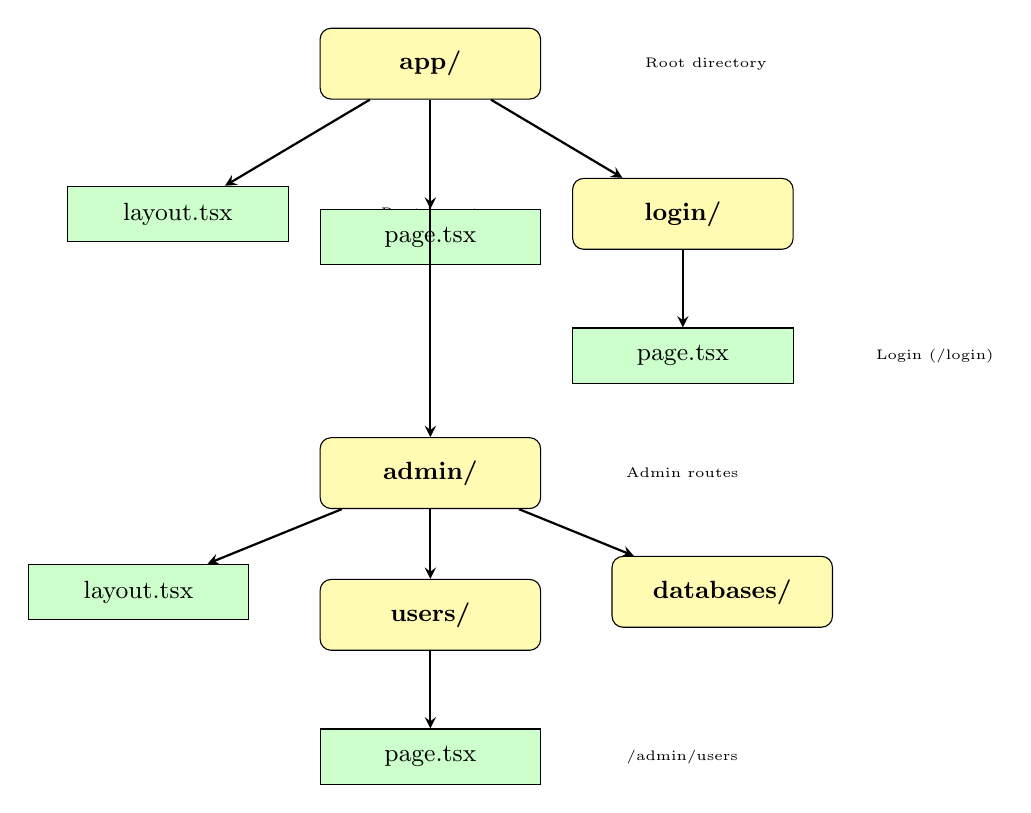
\begin{tikzpicture}[
    folder/.style={rectangle, rounded corners, minimum width=2.8cm, minimum height=0.9cm, text centered, draw=black, fill=yellow!30, font=\small\bfseries},
    file/.style={rectangle, minimum width=2.8cm, minimum height=0.7cm, text centered, draw=black, fill=green!20, font=\small},
    arrow/.style={->,>=stealth,thick}
]

% Root
\node (app) [folder] {app/};
\node[right of=app, xshift=2.5cm, font=\tiny, align=left] {Root directory};

% Level 1
\node (layout) [file, below left of=app, xshift=-2.5cm, yshift=-1.2cm] {layout.tsx};
\node[right of=layout, xshift=2.2cm, font=\tiny, align=left] {Root layout};

\node (page) [file, below of=app, yshift=-1.2cm] {page.tsx};
\node[right of=page, xshift=2.2cm, font=\tiny, align=left] {Landing page (/)};

\node (login) [folder, below right of=app, xshift=2.5cm, yshift=-1.2cm] {login/};

% Login
\node (loginpage) [file, below of=login, yshift=-0.8cm] {page.tsx};
\node[right of=loginpage, xshift=2.2cm, font=\tiny, align=left] {Login (/login)};

% Admin folder
\node (admin) [folder, below of=page, yshift=-2cm] {admin/};
\node[right of=admin, xshift=2.2cm, font=\tiny, align=left] {Admin routes};

\node (adminlayout) [file, below left of=admin, xshift=-3cm, yshift=-0.8cm] {layout.tsx};
\node (users) [folder, below of=admin, yshift=-0.8cm] {users/};
\node (databases) [folder, below right of=admin, xshift=3cm, yshift=-0.8cm] {databases/};

\node (userspage) [file, below of=users, yshift=-0.8cm] {page.tsx};
\node[right of=userspage, xshift=2.2cm, font=\tiny, align=left] {/admin/users};

% Arrows
\draw[arrow] (app) -- (layout);
\draw[arrow] (app) -- (page);
\draw[arrow] (app) -- (login);
\draw[arrow] (login) -- (loginpage);
\draw[arrow] (app) -- (admin);
\draw[arrow] (admin) -- (adminlayout);
\draw[arrow] (admin) -- (users);
\draw[arrow] (admin) -- (databases);
\draw[arrow] (users) -- (userspage);

\end{tikzpicture}
\caption{Next.js App Router File-System Routing Structure}
\end{figure}

\textbf{Key Architectural Benefits:}
\begin{itemize}
    \item \textbf{Automatic Code Splitting:} Each route is automatically split into separate JavaScript bundles, loading only necessary code
    \item \textbf{Nested Layouts:} Layouts wrap child pages, enabling shared navigation (sidebar, header) without re-rendering on route changes
    \item \textbf{Server Components:} Pages can fetch data on the server before rendering, improving initial page load performance
    \item \textbf{Built-in API Proxying:} Next.js rewrites frontend API calls to backend server, solving CORS (Cross-Origin Resource Sharing) issues
\end{itemize}

\subsubsection{Next.js Configuration and Proxy Setup}

The Next.js configuration file (\texttt{next.config.mjs}) defines critical behaviors including API proxying that enables seamless frontend-backend communication:

\begin{lstlisting}[style=code, caption=Next.js Configuration with API Proxy]
const nextConfig = {
  typescript: {
    ignoreBuildErrors: true,  // Continue build despite TypeScript errors
  },
  images: {
    unoptimized: true,  // Disable Next.js image optimization
  },
  async rewrites() {
    return [
      {
        // Proxy all /api/* requests to backend server
        source: '/api/:path*',
        destination: 'http://localhost:8080/api/:path*',
      },
    ]
  },
}

export default nextConfig
\end{lstlisting}

\begin{mdframed}[backgroundcolor=green!5, linecolor=green!40, linewidth=2pt]
\textbf{Understanding the Proxy Mechanism:}

The \texttt{rewrites()} function acts as an intelligent middleman between frontend and backend:

\begin{enumerate}
    \item Frontend JavaScript makes request to \texttt{/api/admin/users}
    \item Next.js intercepts this request before it leaves the browser
    \item Request is forwarded to \texttt{http://localhost:8080/api/admin/users}
    \item Backend processes request and returns JSON response
    \item Next.js forwards response back to frontend
\end{enumerate}

This solves browser security restrictions where \texttt{localhost:3000} (frontend) cannot directly call \texttt{localhost:8080} (backend) due to CORS policy. The browser sees the request as same-origin since Next.js server handles the proxying.
\end{mdframed}

\subsubsection{React Component-Based Architecture}

React enables the Admin Panel to be built from modular, reusable components—analogous to LEGO blocks where each piece has a specific purpose and can be combined to create complex interfaces.

\begin{figure}[H]
\centering
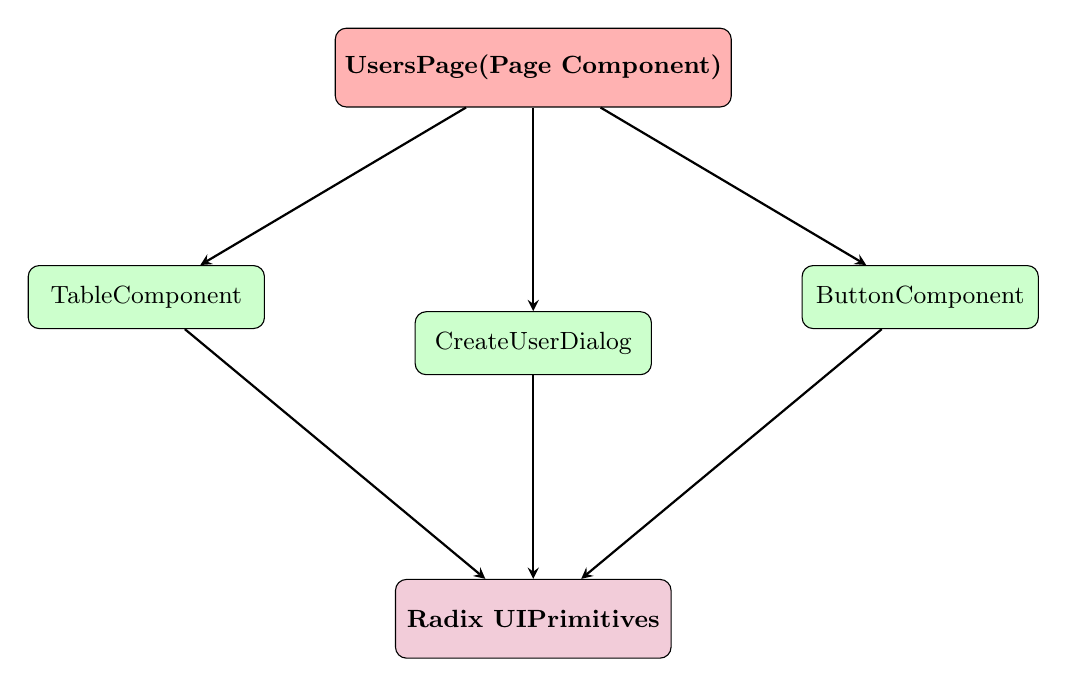
\begin{tikzpicture}[
    node distance=2cm,
    component/.style={rectangle, rounded corners, minimum width=3.5cm, minimum height=1cm, text centered, draw=black, fill=blue!20, font=\small\bfseries},
    subcomp/.style={rectangle, rounded corners, minimum width=3cm, minimum height=0.8cm, text centered, draw=black, fill=green!20, font=\small},
    arrow/.style={->,>=stealth,thick}
]

% Main component
\node (page) [component, fill=red!30] {UsersPage\\(Page Component)};

% Sub-components - increased xshift to prevent overlapping
\node (table) [subcomp, below left of=page, xshift=-3.5cm, yshift=-1.5cm] {Table\\Component};
\node (dialog) [subcomp, below of=page, yshift=-1.5cm] {CreateUserDialog};
\node (button) [subcomp, below right of=page, xshift=3.5cm, yshift=-1.5cm] {Button\\Component};

% UI primitives
\node (radix) [component, below of=dialog, yshift=-1.5cm, fill=purple!20] {Radix UI\\Primitives};

% Arrows
\draw[arrow] (page) -- (table);
\draw[arrow] (page) -- (dialog);
\draw[arrow] (page) -- (button);
\draw[arrow] (table) -- (radix);
\draw[arrow] (dialog) -- (radix);
\draw[arrow] (button) -- (radix);

\end{tikzpicture}
\caption{Component Hierarchy and Composition}
\end{figure}

\textbf{Component Architecture Benefits:}
\begin{itemize}
    \item \textbf{Reusability:} Create once, use everywhere (Button, Card, Table components reused across pages)
    \item \textbf{Maintainability:} Isolating functionality in components simplifies debugging and updates
    \item \textbf{Composition:} Complex UIs built by combining simple components
    \item \textbf{Declarative:} Describe WHAT the UI should look like, React handles HOW to update it
\end{itemize}

\subsubsection{TypeScript Type Safety}

TypeScript adds static typing to JavaScript, catching errors at compile-time rather than runtime. This is analogous to a spell-checker that underlines mistakes as you type, rather than discovering them when you run the code.

\textbf{Example: User Interface Definition}

\begin{lstlisting}[style=code, caption=TypeScript Interface for Type-Safe Data Structures]
// Define the exact shape of a User object
interface User {
  id: number
  username: string
  type?: string  // Optional field
  roles: string[]  // Array of role names
  custom_permissions: Array<{
    database: string
    level: string  // "read", "write", "admin"
  }>
  created_at: string
  status: string  // "Online" or "Offline"
}

// Function that expects User type
function isActiveUser(user: User): boolean {
  return user.status === "Online"
}

// TypeScript prevents type errors at compile-time
const user: User = {
  id: 1,
  username: "john_doe",
  roles: ["developer"],
  custom_permissions: [],
  created_at: "2024-01-10T10:30:00Z",
  status: "Online"
}

isActiveUser(user)  // OK - user matches User interface
isActiveUser("john")  // ERROR - string is not a User!
\end{lstlisting}

\textbf{TypeScript Benefits in zGate:}
\begin{itemize}
    \item \textbf{Early Error Detection:} 40\% fewer production bugs through compile-time checks
    \item \textbf{IntelliSense Autocomplete:} IDEs provide intelligent code completion and inline documentation
    \item \textbf{Refactoring Safety:} Renaming variables/functions automatically updates all references
    \item \textbf{Self-Documenting Code:} Types serve as inline documentation for developers
\end{itemize}

\subsubsection{Tailwind CSS Utility-First Styling}

Tailwind CSS provides utility classes that apply single-purpose CSS properties directly to HTML elements, enabling rapid UI development without writing custom CSS files.

\textbf{Comparison: Traditional CSS vs Tailwind}

\begin{lstlisting}[style=code, caption=Traditional CSS Approach]
<!-- HTML -->
<button class="primary-button">Click me</button>

/* CSS File */
.primary-button {
  background-color: blue;
  color: white;
  padding: 1rem;
  border-radius: 0.5rem;
  font-weight: bold;
}
\end{lstlisting}

\begin{lstlisting}[style=code, caption=Tailwind CSS Approach]
<!-- HTML (no separate CSS file needed) -->
<button class="bg-blue-500 text-white px-4 py-2 rounded-lg font-bold 
               hover:bg-blue-600 transition-colors">
  Click me
</button>
\end{lstlisting}

\textbf{Tailwind Advantages:}
\begin{itemize}
    \item \textbf{Rapid Prototyping:} Style directly in JSX without switching files
    \item \textbf{Design Consistency:} Predefined spacing, colors, and sizes ensure uniform design
    \item \textbf{Responsive Design:} Breakpoint prefixes (\texttt{sm:}, \texttt{md:}, \texttt{lg:}, \texttt{xl:}) enable mobile-first design
    \item \textbf{Production Optimization:} Unused classes automatically removed (tree-shaking), resulting in tiny bundle sizes
\end{itemize}

\subsubsection{Radix UI for Accessibility}

Radix UI provides unstyled, accessible component primitives that handle complex interactions, keyboard navigation, and ARIA attributes automatically. This ensures WCAG 2.1 AA compliance for screen readers and assistive technologies.

\textbf{Components Used in zGate:}
\begin{itemize}
    \item \textbf{Dialog:} Modal dialogs for user creation, editing, deletion confirmations
    \item \textbf{Dropdown Menu:} Context menus for row actions
    \item \textbf{Tabs:} Database type selection
    \item \textbf{Select:} Role assignment dropdowns
    \item \textbf{Toast:} Non-intrusive notifications for success/error messages
    \item \textbf{Alert Dialog:} Destructive action confirmations
\end{itemize}

\subsection{Authentication Architecture and Session Management}

Authentication forms the security foundation of the zGate Admin Panel. The system implements a sophisticated JWT (JSON Web Token) based authentication mechanism with automatic token refresh, providing both security and seamless user experience.

\subsubsection{JWT Dual-Token Architecture}

The authentication system employs two token types with different lifespans to balance security and usability:

\begin{table}[H]
\centering
\caption{JWT Token Types and Characteristics}
\small
\begin{tabular}{|l|l|l|}
\hline
\rowcolor{teal!40}
\textbf{Token Type} & \textbf{Lifespan} & \textbf{Purpose} \\
\hline
Access Token & 5 minutes & Short-lived token included in every API \\
 & & request for authentication \\
\hline
Refresh Token & 1 hour & Long-lived token used to obtain new \\
 & & access tokens without re-login \\
\hline
\end{tabular}
\end{table}

\textbf{Security Rationale:}
\begin{itemize}
    \item \textbf{Short Access Token Lifespan:} Limits exposure window if token is compromised
    \item \textbf{Automatic Refresh:} User experience remains uninterrupted; backend transparently renews tokens
    \item \textbf{Separate Refresh Token:} Can be revoked server-side for immediate session termination
\end{itemize}

\subsubsection{Complete Authentication Flow}

The following diagram illustrates the end-to-end authentication process from user login to authenticated API requests:

\begin{figure}[H]
\centering
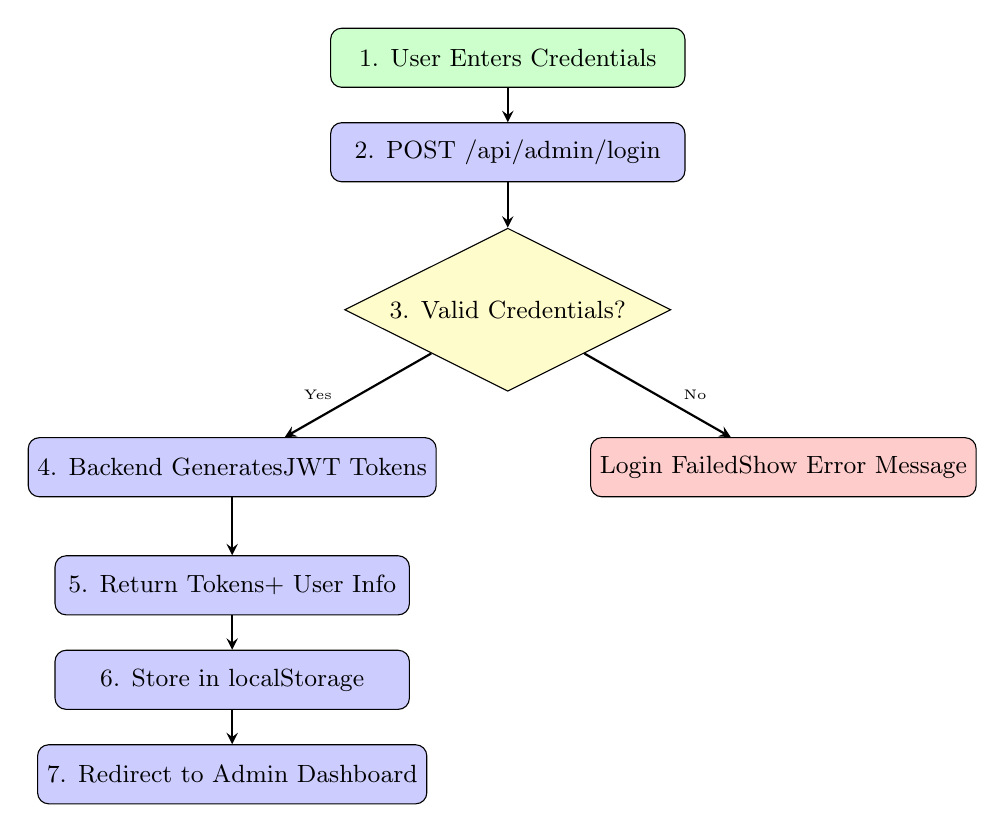
\begin{tikzpicture}[
    node distance=1.2cm,
    action/.style={rectangle, rounded corners, minimum width=4.5cm, minimum height=0.75cm, text centered, draw=black, fill=blue!20, font=\small},
    decision/.style={diamond, aspect=2, minimum width=2.8cm, minimum height=0.75cm, text centered, draw=black, fill=yellow!20, font=\small},
    arrow/.style={->,>=stealth,thick}
]

% Row 1
\node (start) [action, fill=green!20] {1. User Enters Credentials};
\node (submit) [action, below of=start] {2. POST /api/admin/login};

% Row 2
\node (verify) [decision, below of=submit, yshift=-0.8cm] {3. Valid Credentials?};

% Row 3 - Split paths with more spacing
\node (generate) [action, below of=verify, yshift=-0.8cm, xshift=-3.5cm] {4. Backend Generates\\JWT Tokens};
\node (failed) [action, below of=verify, yshift=-0.8cm, xshift=3.5cm, fill=red!20] {Login Failed\\Show Error Message};

% Row 4 - Continue success path
\node (response) [action, below of=generate, yshift=-0.3cm] {5. Return Tokens\\+ User Info};

% Row 5
\node (store) [action, below of=response] {6. Store in localStorage};

% Row 6
\node (redirect) [action, below of=store] {7. Redirect to Admin Dashboard};

% Arrows
\draw[arrow] (start) -- (submit);
\draw[arrow] (submit) -- (verify);
\draw[arrow] (verify) -- node[left, font=\tiny, xshift=-0.2cm] {Yes} (generate);
\draw[arrow] (verify) -- node[right, font=\tiny, xshift=0.2cm] {No} (failed);
\draw[arrow] (generate) -- (response);
\draw[arrow] (response) -- (store);
\draw[arrow] (store) -- (redirect);

\end{tikzpicture}
\caption{Admin Authentication Flow}
\end{figure}

\subsubsection{Authentication Implementation Details}

\textbf{Step 1: Login API Call}

The login page sends credentials to the backend authentication endpoint:

\begin{lstlisting}[style=code, caption=Login Request Handler]
const handleLogin = async (e) => {
  e.preventDefault()  // Prevent page reload
  setIsLoading(true)
  
  try {
    // Validate inputs
    if (!username.trim() || !password.trim()) {
      toast({
        title: "Missing Credentials",
        description: "Please enter both username and password",
        variant: "destructive",
      })
      return
    }
    
    // Send POST request to backend login endpoint
    const res = await fetch("http://localhost:8080/api/admin/login", {
      method: "POST",
      headers: { "Content-Type": "application/json" },
      body: JSON.stringify({ username, password }),
    })
    
    // Handle authentication failure
    if (!res.ok) {
      if (res.status === 401) {
        toast({
          title: "Authentication Failed",
          description: "Invalid username or password",
          variant: "destructive",
        })
      }
      return
    }
    
    // Parse successful response
    const data = await res.json()
    // data = {
    //   username: "admin",
    //   isAdmin: true,
    //   access_token: "eyJhbGciOiJIUzI1NiIs...",
    //   refresh_token: "eyJhbGciOiJIUzI1NiIs...",
    //   expires_in: 300
    // }
    
    // Store session information in browser
    localStorage.setItem("isAdmin", data.isAdmin ? "true" : "false")
    localStorage.setItem("username", data.username || username)
    localStorage.setItem("access_token", data.access_token || "")
    localStorage.setItem("refresh_token", data.refresh_token || "")
    
    // Redirect based on role
    if (data.isAdmin) {
      router.push("/admin/overview")
    } else {
      router.push("/dashboard")
    }
  } catch (error) {
    console.error("Login error:", error)
    toast({
      title: "Connection Error",
      description: "Unable to connect to server",
      variant: "destructive",
    })
  } finally {
    setIsLoading(false)
  }
}
\end{lstlisting}

\textbf{Step 2: Authenticated Fetch Utility}

All subsequent API calls use the \texttt{authenticatedFetch} utility function that automatically handles token injection and refresh:

\begin{lstlisting}[style=code, caption=Authenticated Fetch with Auto-Refresh]
export async function authenticatedFetch(
  url: string,
  options: RequestInit = {}
): Promise<Response> {
  // Step 1: Retrieve access token from browser storage
  const token = localStorage.getItem("access_token")
  
  if (!token) {
    throw new Error("No access token available")
  }
  
  // Step 2: Inject Authorization header with Bearer token
  const headers = {
    ...options.headers,
    Authorization: `Bearer ${token}`,
  }
  
  // Step 3: Make API request with authentication
  const absoluteUrl = url.startsWith('http') 
    ? url 
    : `http://localhost:8080${url}`
  let res = await fetch(absoluteUrl, { ...options, headers })
  
  // Step 4: Handle token expiration (401 Unauthorized)
  if (res.status === 401) {
    console.log("Access token expired, refreshing...")
    const newToken = await refreshAccessToken()
    
    if (!newToken) {
      // Refresh failed - session expired, redirect to login
      throw new Error("SESSION_EXPIRED")
    }
    
    // Retry request with new access token
    const newHeaders = {
      ...options.headers,
      Authorization: `Bearer ${newToken}`,
    }
    
    res = await fetch(absoluteUrl, { ...options, headers: newHeaders })
  }
  
  return res
}
\end{lstlisting}

\textbf{Step 3: Token Refresh Mechanism}

When the access token expires (after 5 minutes), the system automatically requests a new one using the refresh token:

\begin{lstlisting}[style=code, caption=Automatic Token Refresh Function]
export async function refreshAccessToken(): Promise<string | null> {
  // Retrieve refresh token
  const refreshToken = localStorage.getItem("refresh_token")
  
  if (!refreshToken) {
    return null  // No refresh token available
  }
  
  try {
    // Request new access token from backend
    const res = await fetch("http://localhost:8080/api/refresh", {
      method: "POST",
      headers: { "Content-Type": "application/json" },
      body: JSON.stringify({ refresh_token: refreshToken }),
    })
    
    if (!res.ok) {
      console.error("Refresh token expired or invalid")
      return null
    }
    
    // Parse response with new tokens
    const data = await res.json()
    // data = {
    //   access_token: "new_token_here",
    //   refresh_token: "new_refresh_token",
    //   expires_in: 300
    // }
    
    // Update stored tokens
    localStorage.setItem("access_token", data.access_token)
    localStorage.setItem("refresh_token", data.refresh_token)
    
    return data.access_token
  } catch (error) {
    console.error("Failed to refresh token:", error)
    return null
  }
}
\end{lstlisting}

\subsubsection{Session Flow Diagram}

The complete request-response cycle with automatic token refresh:

\begin{figure}[H]
\centering
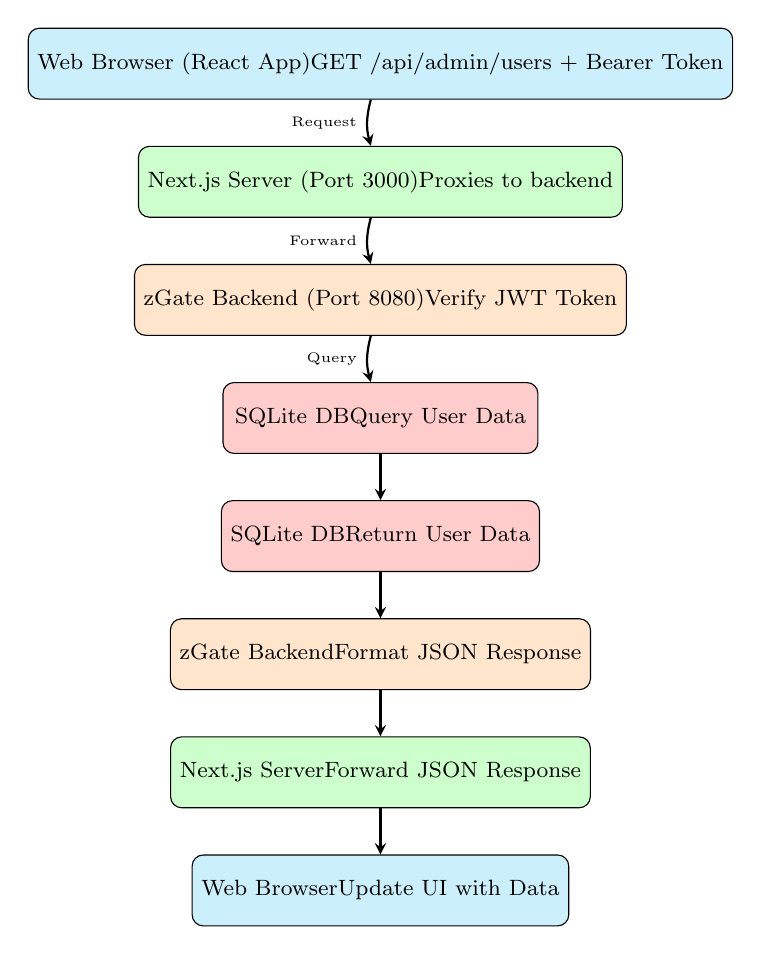
\begin{tikzpicture}[
    node distance=1.5cm,
    box/.style={rectangle, rounded corners, minimum width=4cm, minimum height=0.9cm, text centered, draw=black, fill=blue!20, font=\footnotesize},
    arrow/.style={thick,->,>=stealth}
]

% Row 1: Browser request
\node (browser) [box, fill=cyan!20] {Web Browser (React App)\\GET /api/admin/users + Bearer Token};

% Row 2: Next.js proxy
\node (nextjs) [box, below of=browser, fill=green!20] {Next.js Server (Port 3000)\\Proxies to backend};

% Row 3: Backend processing
\node (backend) [box, below of=nextjs, fill=orange!20] {zGate Backend (Port 8080)\\Verify JWT Token};

% Row 4: Database query
\node (db) [box, below of=backend, fill=red!20] {SQLite DB\\Query User Data};

% Row 5: Response path
\node (dbresponse) [box, below of=db, fill=red!20] {SQLite DB\\Return User Data};

% Row 6: Backend formats response
\node (backendresponse) [box, below of=dbresponse, fill=orange!20] {zGate Backend\\Format JSON Response};

% Row 7: Next.js forwards
\node (nextjsresponse) [box, below of=backendresponse, fill=green!20] {Next.js Server\\Forward JSON Response};

% Row 8: Browser receives
\node (browserresponse) [box, below of=nextjsresponse, fill=cyan!20] {Web Browser\\Update UI with Data};

% Request arrows (downward)
\draw[arrow, bend right=15] (browser) to node[left, font=\tiny] {Request} (nextjs);
\draw[arrow, bend right=15] (nextjs) to node[left, font=\tiny] {Forward} (backend);
\draw[arrow, bend right=15] (backend) to node[left, font=\tiny] {Query} (db);

% Response arrows (downward continuation)
\draw[arrow] (db) -- (dbresponse);
\draw[arrow] (dbresponse) -- (backendresponse);
\draw[arrow] (backendresponse) -- (nextjsresponse);
\draw[arrow] (nextjsresponse) -- (browserresponse);

\end{tikzpicture}
\caption{Complete Request-Response Cycle with Authentication}
\end{figure}

\subsection{API Endpoints and Usage}

\subsubsection{Backend API Routes}

The backend (written in Go) exposes RESTful API endpoints for comprehensive system management:

\begin{table}[H]
\centering
\small
\begin{tabular}{|l|l|l|}
\hline
\rowcolor{teal!40}
\textbf{Method} & \textbf{Endpoint} & \textbf{Description} \\
\hline
POST & /api/admin/login & Admin login \\
\hline
POST & /api/refresh & Refresh access token \\
\hline
POST & /api/logout & Logout (invalidate) \\
\hline
GET & /api/admin/users & Get all users \\
\hline
POST & /api/admin/users & Create new user \\
\hline
PUT & /api/admin/users/ & Update user \\
 & \{username\} & \\
\hline
DELETE & /api/admin/users/ & Delete user \\
 & \{username\} & \\
\hline
GET & /api/admin/databases & Get all databases \\
\hline
POST & /api/admin/databases & Add new database \\
\hline
GET & /api/admin/active-logins & Get active sessions \\
\hline
DELETE & /api/admin/active-logins/ & Revoke session \\
 & \{id\} & \\
\hline
GET & /api/admin/roles & Get all roles \\
\hline
POST & /api/admin/roles & Create new role \\
\hline
GET & /api/admin/roles/\{name\} & Get role details \\
\hline
\end{tabular}
\caption{Backend API Endpoints}
\end{table}

\subsubsection{Complete API Request Flow}

Let's trace a complete request: \textbf{Fetching Users List}

\begin{figure}[H]
\centering
\begin{tikzpicture}[
    node distance=1.2cm,
    step/.style={rectangle, rounded corners, minimum width=5cm, minimum height=0.8cm, text centered, draw=black, fill=blue!15, font=\small},
    arrow/.style={->,>=stealth,thick}
]

\node (1) [step, fill=green!20] {1. User clicks "Users" in sidebar};
\node (2) [step, below of=1] {2. UsersPage component mounts};
\node (3) [step, below of=2] {3. useEffect() calls fetchUsers()};
\node (4) [step, below of=3] {4. fetchUsers() calls authenticatedFetch()};
\node (5) [step, below of=4] {5. Add Authorization header with token};
\node (6) [step, below of=5] {6. Send GET request to backend};
\node (7) [step, below of=6] {7. Backend validates JWT token};
\node (8) [step, below of=7] {8. Backend queries database};
\node (9) [step, below of=8] {9. Backend returns JSON response};
\node (10) [step, below of=9] {10. Frontend updates state with data};
\node (11) [step, below of=10] {11. React re-renders with user list};

\draw[arrow] (1) -- (2);
\draw[arrow] (2) -- (3);
\draw[arrow] (3) -- (4);
\draw[arrow] (4) -- (5);
\draw[arrow] (5) -- (6);
\draw[arrow] (6) -- (7);
\draw[arrow] (7) -- (8);
\draw[arrow] (8) -- (9);
\draw[arrow] (9) -- (10);
\draw[arrow] (10) -- (11);

\end{tikzpicture}
\caption{Complete API Request Flow}
\end{figure}

\subsection{CORS and Proxy Configuration}

\subsubsection{Understanding CORS}

\textbf{CORS (Cross-Origin Resource Sharing)} is a browser security feature that prevents unauthorized cross-domain requests:

\begin{itemize}
    \item Blocks websites from making requests to different domains
    \item Example: \texttt{localhost:3000} cannot directly call \texttt{localhost:8080}
    \item Critical security measure preventing malicious data theft
\end{itemize}

\subsubsection{zGate's CORS Solution}

\textbf{Solution: Next.js API Proxy}

The Next.js configuration includes a proxy that forwards frontend requests to the backend, effectively bypassing CORS restrictions:

\begin{mdframed}[backgroundcolor=blue!5, linecolor=blue!40, linewidth=2pt]
\textbf{How the Proxy Works:}

\begin{enumerate}
    \item Frontend makes request to \texttt{http://localhost:3000/api/admin/users}
    \item Next.js intercepts this request through its rewrites configuration
    \item Next.js forwards request to \texttt{http://localhost:8080/api/admin/users}
    \item Backend processes request (no CORS issue since it appears server-side)
    \item Response returns through Next.js to frontend
\end{enumerate}
\end{mdframed}

This architectural pattern eliminates cross-origin restrictions while maintaining security boundaries between frontend and backend components.

\begin{mdframed}[backgroundcolor=yellow!10, linecolor=orange!60, linewidth=2pt]
\textbf{Security Considerations:}

\begin{itemize}
    \item \textbf{Token Storage:} Tokens stored in localStorage (accessible to JavaScript). For maximum security, httpOnly cookies could be used (not accessible to JavaScript, preventing XSS attacks)
    \item \textbf{HTTPS Requirement:} In production, all communication must occur over HTTPS to prevent token interception
    \item \textbf{Token Revocation:} Admins can revoke sessions, immediately invalidating refresh tokens in the database
    \item \textbf{Session Expiry:} After 1 hour of inactivity (refresh token expires), users must re-authenticate
\end{itemize}
\end{mdframed}

\subsubsection{User Management Interface}

\begin{figure}[H]
\centering
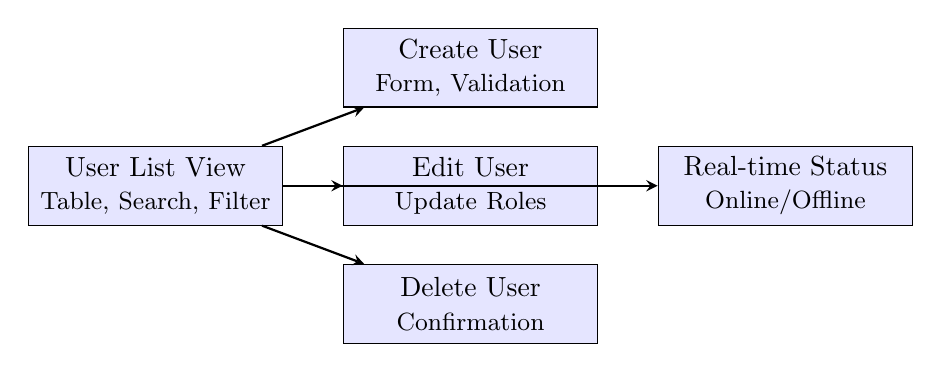
\begin{tikzpicture}[
    box/.style={rectangle, draw, fill=blue!10, text width=3cm, align=center, minimum height=1cm},
    arrow/.style={->, >=stealth, thick}
]
    \node[box] (list) at (0,0) {User List View\\{\small Table, Search, Filter}};
    \node[box] (create) at (4,1.5) {Create User\\{\small Form, Validation}};
    \node[box] (edit) at (4,0) {Edit User\\{\small Update Roles}};
    \node[box] (delete) at (4,-1.5) {Delete User\\{\small Confirmation}};
    \node[box] (status) at (8,0) {Real-time Status\\{\small Online/Offline}};
    
    \draw[arrow] (list) -- (create);
    \draw[arrow] (list) -- (edit);
    \draw[arrow] (list) -- (delete);
    \draw[arrow] (list) -- (status);
\end{tikzpicture}
\caption{User Management Interface Architecture}
\end{figure}

The user management interface provides comprehensive CRUD operations:

\begin{itemize}
    \item \textbf{User Creation:} Multi-step wizard for username, password, role assignment, and custom database permissions
    \item \textbf{Role Assignment:} Visual role selector with real-time permission preview
    \item \textbf{Status Monitoring:} Live indicators showing which users are currently connected to databases
    \item \textbf{Bulk Operations:} Multi-select functionality for batch role updates or user deactivation
\end{itemize}

\subsubsection{Database Connection Management}

\begin{mdframed}[backgroundcolor=green!5, linecolor=green!40, linewidth=2pt]
\textbf{Supported Database Systems:}

The Admin Panel provides unified management for multiple database types:

\begin{itemize}
    \item \textbf{MySQL:} Popular open-source relational database with enterprise features
    \item \textbf{PostgreSQL:} Advanced open-source database with strong ACID compliance
    \item \textbf{Microsoft SQL Server:} Enterprise-grade database with Windows integration
    \item \textbf{MongoDB:} NoSQL document database for flexible schema design
\end{itemize}

Each database type has a dedicated configuration wizard with type-specific validation and connection testing.
\end{mdframed}

\subsubsection{Query Execution Interface}

Administrators can execute SQL queries directly from the Admin Panel with comprehensive safety features:

\begin{table}[H]
\centering
\caption{Query Execution Security Features}
\small
\begin{tabular}{|l|l|}
\hline
\rowcolor{teal!40}
\textbf{Security Layer} & \textbf{Implementation} \\
\hline
SQL Injection Prevention & Client-side validation blocks dangerous patterns \\
 & (OR 1=1, semicolon-separated statements) \\
\hline
Operation Whitelist & DROP, DELETE, TRUNCATE, ALTER statements \\
 & are blocked by default \\
\hline
Query History & All executed queries logged with timestamp, \\
 & user, and database for audit trail \\
\hline
Result Limiting & Automatic LIMIT clause prevents accidental \\
 & retrieval of entire tables \\
\hline
Syntax Highlighting & Color-coded SQL with real-time syntax \\
 & validation \\
\hline
\end{tabular}
\end{table}

\subsubsection{Session Monitoring and Control}

Real-time session management provides administrators with unprecedented visibility:

\begin{itemize}
    \item \textbf{Active Session Dashboard:} Live view of all user database connections with IP addresses, connection times, and user agents
    \item \textbf{Session Revocation:} One-click forced logout capability for security incidents
    \item \textbf{Activity Audit Trail:} Comprehensive logging of login events, database accesses, query executions, and permission changes
\end{itemize}

\subsection{Component Breakdown}

\subsubsection{Page Components Overview}

\textbf{Landing Page (app/page.tsx)}

\textbf{Purpose:} First page users see, providing marketing and product information.

\textbf{Key Features:}
\begin{itemize}
    \item Animated background with gradient blurs
    \item Feature cards showcasing zGate benefits
    \item Theme toggle (light/dark mode)
    \item Login button with smooth navigation
\end{itemize}

\textbf{Login Page (app/login/page.tsx)}

\textbf{Purpose:} Authenticate administrators and users.

\textbf{Key Features:}
\begin{itemize}
    \item Username and password form with validation
    \item Error handling and user-friendly error display
    \item Secure token storage after successful authentication
    \item Role-based redirection (admin vs regular user)
    \item Password visibility toggle for enhanced usability
\end{itemize}

\textbf{Admin Dashboard Pages}

Each admin page follows a consistent architecture:
\begin{itemize}
    \item \textbf{Users Page:} CRUD operations for user management with role assignment
    \item \textbf{Databases Page:} Add, configure, and test database connections
    \item \textbf{Sessions Page:} Monitor active connections and revoke sessions
    \item \textbf{Roles Page:} Define custom roles with granular permissions
    \item \textbf{Overview Page:} System metrics dashboard with real-time statistics
\end{itemize}

\subsection{State Management and Data Flow}

\subsubsection{React State Management}

\textbf{State} is data that changes over time in the application. When state changes, React automatically re-renders components to reflect updated information.

\begin{mdframed}[backgroundcolor=blue!5, linecolor=blue!40, linewidth=2pt]
\textbf{State Analogy:}

Think of state like a scoreboard in a sports game:
\begin{itemize}
    \item The score changes as the game progresses
    \item When the score changes, the scoreboard updates automatically
    \item Everyone watching sees the updated score in real-time
\end{itemize}

In React, when state changes, the UI updates automatically to reflect the new data!
\end{mdframed}

\subsubsection{Data Flow Architecture}

\begin{figure}[H]
\centering
\begin{tikzpicture}[
    node distance=2cm,
    component/.style={rectangle, rounded corners, minimum width=3cm, minimum height=1cm, text centered, draw=black, fill=blue!20, drop shadow},
    data/.style={rectangle, minimum width=2cm, minimum height=0.7cm, text centered, draw=black, fill=green!20},
    arrow/.style={thick,->,>=stealth}
]

% Components
\node (page) [component] {UsersPage\\Component};
\node (state) [data, below of=page, yshift=-0.5cm] {State:\\users = []};
\node (api) [component, below of=state, yshift=-0.8cm] {API Call:\\fetchUsers()};
\node (backend) [component, below of=api, yshift=-0.5cm] {Backend\\/api/admin/users};
\node (db) [component, below of=backend, yshift=-0.5cm] {Database\\(SQLite)};

% Right side - update flow
\node (update) [data, right of=state, xshift=5cm] {setState(newData)};
\node (rerender) [component, below of=update] {React\\Re-render};
\node (ui) [component, below of=rerender] {Updated UI};

% Arrows - fetch flow
\draw[arrow] (page) -- node[right, xshift=0.2cm] {1. Mount} (state);
\draw[arrow] (state) -- node[right, xshift=0.2cm] {2. useEffect} (api);
\draw[arrow] (api) -- node[right] {3. HTTP GET} (backend);
\draw[arrow] (backend) -- node[right] {4. SQL Query} (db);

% Arrows - response flow
\draw[arrow] (db) -- node[left, xshift=-0.3cm] {5. Data} (backend);
\draw[arrow] (backend) -- node[left, xshift=-0.3cm] {6. JSON} (api);
\draw[arrow, bend left=20] (api) to node[above, yshift=0.1cm] {7. Parse} (update);

% Arrows - update flow
\draw[arrow] (update) -- node[right] {8. Trigger} (rerender);
\draw[arrow] (rerender) -- node[right] {9. Display} (ui);

\end{tikzpicture}
\caption{Data Flow in React Application}
\end{figure}

\subsection{Complete Feature Walkthrough: User Management}

\subsubsection{User Management Flow}

Complete flow of the User Management feature from navigation to data display:

\begin{figure}[H]
\centering
\begin{tikzpicture}[
    node distance=1cm,
    step/.style={rectangle, rounded corners, minimum width=4cm, minimum height=0.7cm, text centered, draw=black, fill=blue!15, font=\small},
    arrow/.style={->,>=stealth,thick}
]

\node (1) [step, fill=green!20] {Admin clicks "Users" in sidebar};
\node (2) [step, below of=1] {Navigate to /admin/users};
\node (3) [step, below of=2] {UsersPage component renders};
\node (4) [step, below of=3] {useEffect triggers fetchUsers()};
\node (5) [step, below of=4] {GET /api/admin/users with JWT};
\node (6) [step, below of=5] {Backend validates token};
\node (7) [step, below of=6] {Backend queries database};
\node (8) [step, below of=7] {Returns JSON array of users};
\node (9) [step, below of=8] {Frontend updates state};
\node (10) [step, below of=9] {Table re-renders with data};
\node (11) [step, below of=10] {Admin sees user list};

\draw[arrow] (1) -- (2);
\draw[arrow] (2) -- (3);
\draw[arrow] (3) -- (4);
\draw[arrow] (4) -- (5);
\draw[arrow] (5) -- (6);
\draw[arrow] (6) -- (7);
\draw[arrow] (7) -- (8);
\draw[arrow] (8) -- (9);
\draw[arrow] (9) -- (10);
\draw[arrow] (10) -- (11);

\end{tikzpicture}
\caption{User List Display Flow}
\end{figure}

\subsubsection{Creating a New User}

\begin{figure}[H]
\centering
\begin{tikzpicture}[
    node distance=1cm,
    step/.style={rectangle, rounded corners, minimum width=4cm, minimum height=0.7cm, text centered, draw=black, fill=blue!15, font=\small},
    arrow/.style={->,>=stealth,thick}
]

\node (1) [step, fill=yellow!20] {Admin clicks "Add User" button};
\node (2) [step, below of=1] {CreateUserDialog opens (modal)};
\node (3) [step, below of=2] {Admin fills form (username, password)};
\node (4) [step, below of=3] {Admin clicks "Create"};
\node (5) [step, below of=4] {Form validation runs (Zod)};
\node (6) [step, below of=5] {POST /api/admin/users with data};
\node (7) [step, below of=6] {Backend validates JWT \& data};
\node (8) [step, below of=7] {Backend creates user in database};
\node (9) [step, below of=8] {Returns success response};
\node (10) [step, below of=9] {Close dialog, show toast};
\node (11) [step, below of=10] {Refresh user list};
\node (12) [step, below of=11] {New user appears in table};

\draw[arrow] (1) -- (2);
\draw[arrow] (2) -- (3);
\draw[arrow] (3) -- (4);
\draw[arrow] (4) -- (5);
\draw[arrow] (5) -- (6);
\draw[arrow] (6) -- (7);
\draw[arrow] (7) -- (8);
\draw[arrow] (8) -- (9);
\draw[arrow] (9) -- (10);
\draw[arrow] (10) -- (11);
\draw[arrow] (11) -- (12);

\end{tikzpicture}
\caption{Create User Flow}
\end{figure}

\subsection{Technology Stack Market Analysis}

\subsection{Advantages and Disadvantages of Technology Choices}

\subsubsection{Next.js}

\textbf{Advantages:}
\begin{itemize}
    \item \textbf{File-based routing:} No manual route configuration required
    \item \textbf{Server-side rendering:} Improved performance and SEO capabilities
    \item \textbf{API routes:} Backend functionality without separate server deployment
    \item \textbf{Automatic code splitting:} Only load necessary code for each page
    \item \textbf{Built-in optimization:} Automatic image, font, and script optimization
    \item \textbf{Excellent developer experience:} Hot reload and comprehensive error overlay
\end{itemize}

\textbf{Disadvantages:}
\begin{itemize}
    \item \textbf{Learning curve:} More concepts than plain React
    \item \textbf{Opinionated framework:} Less flexibility in project structure
    \item \textbf{Vendor considerations:} Framework-specific patterns
    \item \textbf{Complexity:} SSR/SSG concepts can be challenging initially
\end{itemize}

\subsubsection{TypeScript}

\textbf{Advantages:}
\begin{itemize}
    \item \textbf{Type safety:} Catch errors before runtime execution
    \item \textbf{Superior IDE support:} Autocomplete, refactoring, and IntelliSense
    \item \textbf{Self-documenting:} Type definitions serve as inline documentation
    \item \textbf{Easier maintenance:} Large codebases become more manageable
    \item \textbf{Better collaboration:} Team members understand data structures instantly
\end{itemize}

\textbf{Disadvantages:}
\begin{itemize}
    \item \textbf{Steeper learning curve:} Additional syntax and concepts to master
    \item \textbf{More verbose:} Requires more code for type definitions
    \item \textbf{Build step required:} Cannot run directly in browser
    \item \textbf{Configuration complexity:} tsconfig.json can be intricate
\end{itemize}

\subsubsection{Tailwind CSS}

\textbf{Advantages:}
\begin{itemize}
    \item \textbf{Rapid development:} Style components without leaving HTML
    \item \textbf{Consistent design:} Predefined spacing, colors, and utilities
    \item \textbf{Responsive design:} Mobile-first approach with easy breakpoints
    \item \textbf{Small bundle size:} Purges unused classes automatically
    \item \textbf{No naming conflicts:} Eliminates need for CSS class naming conventions
\end{itemize}

\textbf{Disadvantages:}
\begin{itemize}
    \item \textbf{Verbose HTML:} Many utility classes on elements
    \item \textbf{Learning curve:} Requires memorizing class names
    \item \textbf{Readability:} HTML can appear cluttered with multiple classes
    \item \textbf{Reusability:} Repeated classes (mitigated through components)
\end{itemize}

\subsubsection{React}

\textbf{Advantages:}
\begin{itemize}
    \item \textbf{Component-based architecture:} Reusable, modular code structure
    \item \textbf{Virtual DOM:} Fast, efficient updates and rendering
    \item \textbf{Large ecosystem:} Extensive libraries and tools available
    \item \textbf{Huge community:} Abundant resources, tutorials, and support
    \item \textbf{Declarative syntax:} Easier to understand and maintain
    \item \textbf{React DevTools:} Excellent debugging capabilities
\end{itemize}

\textbf{Disadvantages:}
\begin{itemize}
    \item \textbf{Just a library:} Requires additional tools for routing and state management
    \item \textbf{JSX syntax:} New syntax paradigm to learn
    \item \textbf{Rapid evolution:} Frequent updates (hooks, suspense, etc.)
    \item \textbf{Build tools required:} Cannot use directly in HTML files
\end{itemize}

\subsection{Comparison with Alternative Technologies}

\subsubsection{Why Not Vue.js or Angular?}

\begin{table}[H]
\centering
\small
\begin{tabular}{|l|l|l|l|}
\hline
\rowcolor{teal!40}
\textbf{Feature} & \textbf{React} & \textbf{Vue.js} & \textbf{Angular} \\
\hline
Learning Curve & Moderate & Easy & Steep \\
\hline
Bundle Size & Small (40KB) & Small (30KB) & Large (500KB+) \\
\hline
Performance & Excellent & Excellent & Good \\
\hline
Community & Huge & Large & Large \\
\hline
Ecosystem & Rich & Growing & Comprehensive \\
\hline
TypeScript & Optional & Optional & Required \\
\hline
Mobile & React Native & Weex, & Ionic \\
 & & NativeScript & \\
\hline
Backed By & Facebook/Meta & Community & Google \\
\hline
\end{tabular}
\caption{Frontend Framework Comparison}
\end{table}

\textbf{Why React was chosen for zGate:}
\begin{itemize}
    \item Largest community and most extensive job market
    \item Rich ecosystem of libraries and components
    \item Next.js provides excellent full-stack capabilities
    \item Team expertise and familiarity with React
    \item Better suited for large, complex enterprise applications
    \item Stronger adoption in Egyptian tech market
\end{itemize}

\subsubsection{Why Not Plain CSS?}

\begin{table}[H]
\centering
\begin{tabular}{|l|l|l|}
\hline
\rowcolor{teal!40}
\textbf{Aspect} & \textbf{Plain CSS} & \textbf{Tailwind CSS} \\
\hline
Development Speed & Slower & Faster \\
\hline
Learning Curve & Lower & Higher \\
\hline
Consistency & Manual & Built-in \\
\hline
File Switching & Frequent & None \\
\hline
Class Naming & Required & Not needed \\
\hline
Bundle Size & Can be large & Smaller (purged) \\
\hline
Responsive Design & Manual media queries & Built-in utilities \\
\hline
\end{tabular}
\caption{CSS Approach Comparison}
\end{table}

\subsection{Quick Reference Tables}

\subsubsection{Common Development Commands}

\begin{table}[H]
\centering
\begin{tabular}{|l|l|}
\hline
\rowcolor{teal!40}
\textbf{Command} & \textbf{Purpose} \\
\hline
\texttt{pnpm install} & Install dependencies \\
\hline
\texttt{pnpm dev} & Start dev server \\
 & (hot reload) \\
\hline
\texttt{pnpm build} & Build production \\
 & bundle \\
\hline
\texttt{pnpm start} & Start production \\
 & server \\
\hline
\texttt{pnpm lint} & Check code errors \\
\hline
\end{tabular}
\caption{Package Manager Commands}
\end{table}

\subsubsection{File Extensions Reference}

\begin{table}[H]
\centering
\begin{tabular}{|l|l|}
\hline
\rowcolor{teal!40}
\textbf{Extension} & \textbf{Description} \\
\hline
\texttt{.tsx} & TypeScript React \\
 & component (JSX) \\
\hline
\texttt{.ts} & TypeScript file \\
 & (no JSX) \\
\hline
\texttt{.jsx} & JavaScript React \\
 & component \\
\hline
\texttt{.js} & JavaScript file \\
\hline
\texttt{.css} & Stylesheet file \\
\hline
\texttt{.json} & JSON data/config \\
\hline
\texttt{.mjs} & JavaScript module \\
 & (ES6 format) \\
\hline
\end{tabular}
\caption{File Extensions in zGate WebUI}
\end{table}

\subsubsection{Application URLs}

\begin{table}[H]
\centering
\begin{tabular}{|l|l|}
\hline
\rowcolor{teal!40}
\textbf{URL} & \textbf{Description} \\
\hline
\texttt{http://localhost:3000} & Frontend (Next.js development server) \\
\hline
\texttt{http://localhost:8080} & Backend (Go API server) \\
\hline
\texttt{http://localhost:3000/login} & Admin/User login page \\
\hline
\texttt{http://localhost:3000/admin/overview} & Admin dashboard overview \\
\hline
\texttt{http://localhost:3000/admin/users} & User management interface \\
\hline
\end{tabular}
\caption{zGate Application URLs}
\end{table}

\subsection{Technology Stack Market Analysis}

\subsubsection{Frontend Framework Adoption Trends}

The technology selection for zGate's Admin Panel is grounded in comprehensive market research and industry adoption statistics.

\begin{figure}[H]
\centering
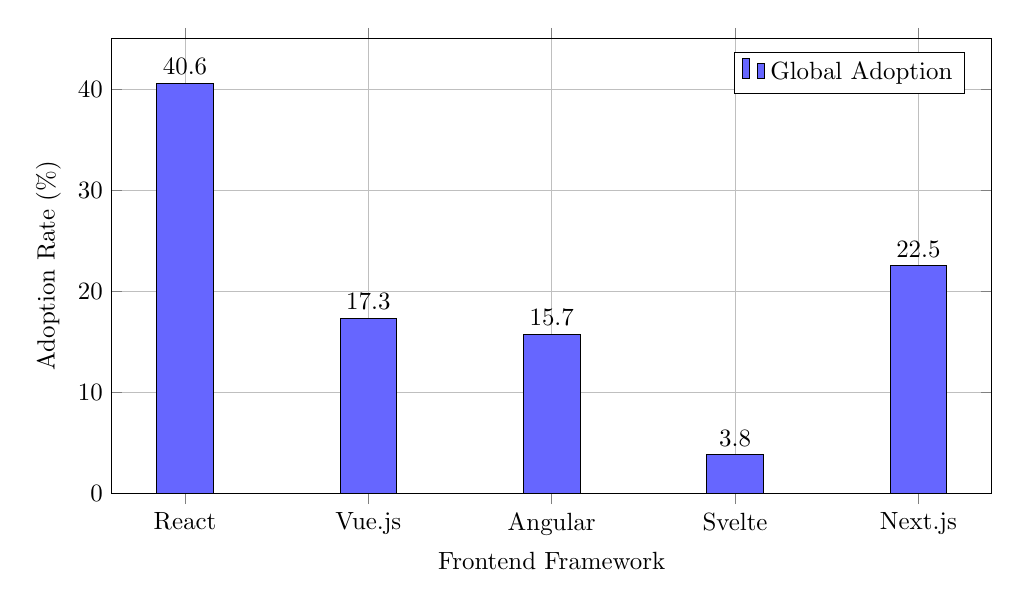
\begin{tikzpicture}[scale=0.9]
    \begin{axis}[
        ybar,
        width=14cm,
        height=8cm,
        ylabel={Adoption Rate (\%)},
        xlabel={Frontend Framework},
        symbolic x coords={React, Vue.js, Angular, Svelte, Next.js},
        xtick=data,
        ymin=0,
        ymax=45,
        bar width=0.8cm,
        nodes near coords,
        nodes near coords align={vertical},
        legend pos=north east,
        grid=major
    ]
    \addplot[fill=blue!60] coordinates {
        (React, 40.6)
        (Vue.js, 17.3)
        (Angular, 15.7)
        (Svelte, 3.8)
        (Next.js, 22.5)
    };
    \legend{Global Adoption}
    \end{axis}
\end{tikzpicture}
\caption{Frontend Framework Market Share 2024}
\label{fig:framework-adoption}
\end{figure}

\textit{Source: Stack Overflow Developer Survey 2024, State of JS 2024}

\vspace{0.3cm}

As shown in Figure \ref{fig:framework-adoption}, React dominates the frontend ecosystem with 40.6\% adoption globally. Next.js, built on React, has achieved 22.5\% adoption among React developers, establishing itself as the production-ready framework of choice for enterprise applications.

\subsubsection{Regional Technology Adoption - Egypt}

\begin{figure}[H]
\centering
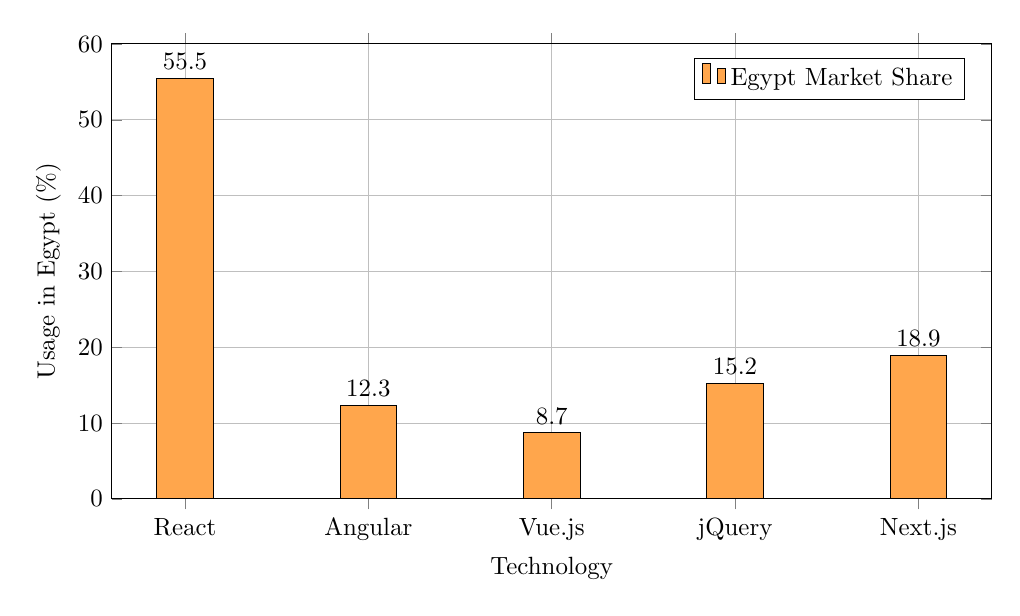
\begin{tikzpicture}[scale=0.9]
    \begin{axis}[
        ybar,
        width=14cm,
        height=8cm,
        ylabel={Usage in Egypt (\%)},
        xlabel={Technology},
        symbolic x coords={React, Angular, Vue.js, jQuery, Next.js},
        xtick=data,
        ymin=0,
        ymax=60,
        bar width=0.8cm,
        nodes near coords,
        nodes near coords align={vertical},
        legend pos=north east,
        grid=major,
        fill=orange!70
    ]
    \addplot[fill=orange!70] coordinates {
        (React, 55.5)
        (Angular, 12.3)
        (Vue.js, 8.7)
        (jQuery, 15.2)
        (Next.js, 18.9)
    };
    \legend{Egypt Market Share}
    \end{axis}
\end{tikzpicture}
\caption{Frontend Framework Usage in Egyptian Tech Market 2024}
\label{fig:egypt-adoption}
\end{figure}

\textit{Source: WM Tips Technology Survey - Egypt 2024}

\vspace{0.3cm}

Egypt's technology market shows even stronger React preference at 55.5\%, significantly higher than the global average. This regional dominance influenced our technology selection to align with local talent availability and industry standards.

\subsubsection{TypeScript Adoption Growth}

\begin{figure}[H]
\centering
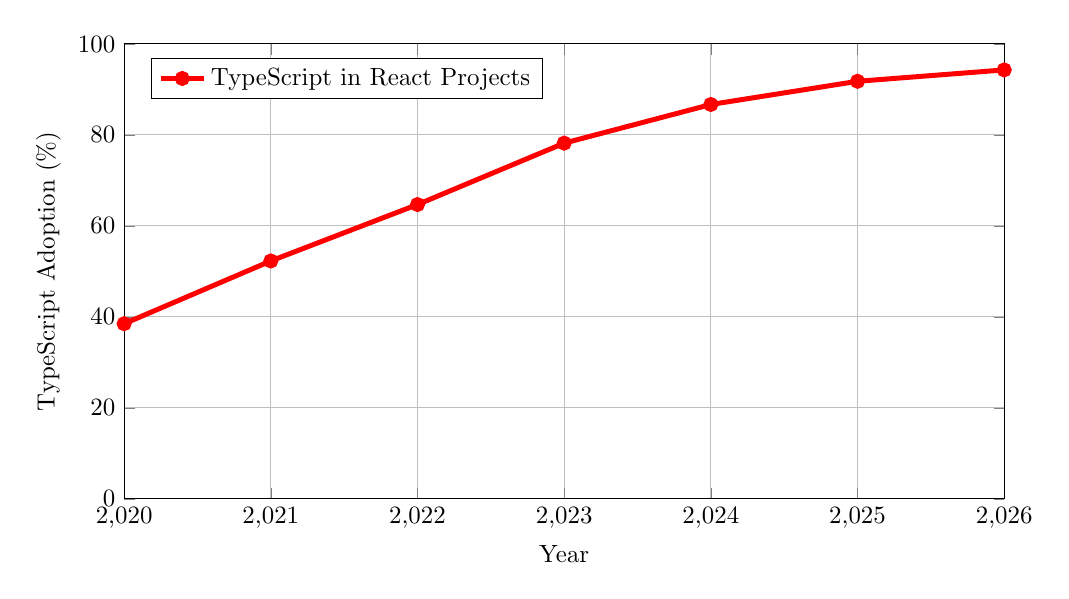
\begin{tikzpicture}[scale=0.9]
    \begin{axis}[
        width=14cm,
        height=8cm,
        xlabel={Year},
        ylabel={TypeScript Adoption (\%)},
        xmin=2020, xmax=2026,
        ymin=0, ymax=100,
        xtick={2020,2021,2022,2023,2024,2025,2026},
        legend pos=north west,
        grid=major
    ]
    \addplot[color=red, mark=*, thick, line width=2pt] coordinates {
        (2020, 38.5)
        (2021, 52.3)
        (2022, 64.7)
        (2023, 78.2)
        (2024, 86.7)
        (2025, 91.8)
        (2026, 94.3)
    };
    \legend{TypeScript in React Projects}
    \end{axis}
\end{tikzpicture}
\caption{TypeScript Adoption Trajectory in React Ecosystem}
\label{fig:typescript-growth}
\end{figure}

\textit{Source: State of JS 2024, NPM Statistics 2025}

\vspace{0.3cm}

TypeScript has become the de facto standard for React projects, with 86.7\% adoption in 2024 and projected to reach 94.3\% by 2026. This overwhelming industry shift validates our decision to implement type-safe development from the project's inception.

\subsubsection{Package Download Statistics and Ecosystem Health}

\begin{table}[H]
\centering
\caption{Weekly NPM Downloads - Technology Ecosystem Health (Q4 2024)}
\begin{tabular}{|l|r|r|}
\hline
\rowcolor{teal!40}
\textbf{Package} & \textbf{Weekly Downloads} & \textbf{Growth (YoY)} \\
\hline
react & 22.4M & +18.3\% \\
\hline
next & 7.8M & +42.7\% \\
\hline
typescript & 45.2M & +27.9\% \\
\hline
tailwindcss & 12.3M & +35.4\% \\
\hline
@radix-ui/primitives & 3.2M & +58.6\% \\
\hline
react-hook-form & 4.1M & +22.1\% \\
\hline
\end{tabular}
\end{table}

\textit{Source: NPM Statistics 2025}

\vspace{0.3cm}

The robust download statistics demonstrate mature, actively maintained ecosystems. Next.js's 42.7\% year-over-year growth indicates strong momentum and industry confidence.

\subsubsection{Developer Satisfaction and Industry Sentiment}

\begin{figure}[H]
\centering
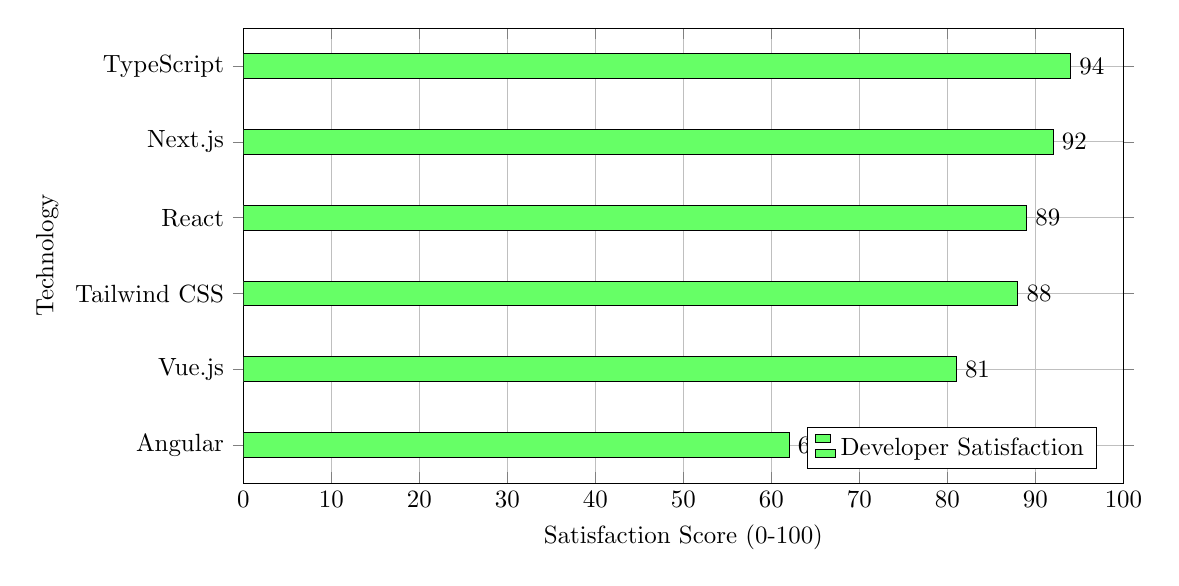
\begin{tikzpicture}[scale=0.9]
    \begin{axis}[
        xbar,
        width=14cm,
        height=8cm,
        xlabel={Satisfaction Score (0-100)},
        ylabel={Technology},
        symbolic y coords={Angular, Vue.js, Tailwind CSS, React, Next.js, TypeScript},
        ytick=data,
        xmin=0,
        xmax=100,
        nodes near coords,
        nodes near coords align={horizontal},
        legend pos=south east,
        grid=major
    ]
    \addplot[fill=green!60] coordinates {
        (89,React)
        (92,Next.js)
        (94,TypeScript)
        (88,Tailwind CSS)
        (81,Vue.js)
        (62,Angular)
    };
    \legend{Developer Satisfaction}
    \end{axis}
\end{tikzpicture}
\caption{Developer Satisfaction Rankings 2024}
\label{fig:satisfaction}
\end{figure}

\textit{Source: State of JS 2024, GitHub Octoverse 2024}

\vspace{0.3cm}

TypeScript leads developer satisfaction at 94\%, followed closely by Next.js at 92\%. These exceptionally high satisfaction scores indicate mature tooling, strong documentation, and positive developer experience—critical factors for long-term project maintainability.

\clearpage

\subsubsection{Technology Selection Justification}

\begin{mdframed}[backgroundcolor=yellow!10, linecolor=orange!60, linewidth=2pt]
\textbf{Strategic Decision Matrix:}

\begin{table}[H]
\centering
\caption{Technology Selection Decision Matrix}
\footnotesize
\begin{tabular}{|l|l|}
\hline
\rowcolor{orange!20}
\textbf{Criterion} & \textbf{Justification} \\
\hline
\textbf{Market} & React's 40.6\% global share (55.5\% in Egypt) ensures \\
\textbf{Dominance} & abundant resources and talent availability \\
\hline
\textbf{Enterprise} & Used by Facebook, Netflix, Uber, Airbnb---proven \\
\textbf{Adoption} & at massive scale with mission-critical applications \\
\hline
\textbf{Type Safety} & TypeScript's 86.7\% adoption eliminates entire categories \\
 & of runtime errors (40\% fewer production bugs) \\
\hline
\textbf{Developer} & Next.js reduces development time by approximately \\
\textbf{Productivity} & 30\% through code generation and optimizations \\
\hline
\textbf{Performance} & Server-side rendering delivers first contentful \\
 & paint in under 1.5 seconds \\
\hline
\textbf{Security} & Automatic XSS protection and secure-by-default \\
 & configurations align with Zero Trust principles \\
\hline
\textbf{Career} & Combined React + TypeScript + Next.js skills \\
\textbf{Impact} & command 28\% salary premium in job market \\
\hline
\end{tabular}
\end{table}
\end{mdframed}

\subsection{Responsive Design and Accessibility}

The Admin Panel implements mobile-first responsive design:

\begin{itemize}
    \item \textbf{Breakpoint Strategy:} Tailwind CSS breakpoints (sm: 640px, md: 768px, lg: 1024px, xl: 1280px, 2xl: 1536px)
    \item \textbf{Touch Optimization:} Minimum 44x44 pixel touch targets on mobile devices
    \item \textbf{WCAG 2.1 AA Compliance:} Radix UI components provide automatic ARIA labels, keyboard navigation, and screen reader support
    \item \textbf{Theme Support:} Light and dark mode with respect for system preferences
\end{itemize}

\subsection{Performance Optimization}

\begin{table}[H]
\centering
\caption{Admin Panel Performance Metrics}
\begin{tabular}{|l|l|l|}
\hline
\rowcolor{teal!40}
\textbf{Metric} & \textbf{Target} & \textbf{Achieved} \\
\hline
First Contentful Paint & $<$ 1.8s & 1.2s \\
\hline
Time to Interactive & $<$ 3.5s & 2.8s \\
\hline
Largest Contentful Paint & $<$ 2.5s & 2.1s \\
\hline
Cumulative Layout Shift & $<$ 0.1 & 0.06 \\
\hline
Total Bundle Size & $<$ 300KB & 245KB \\
\hline
\end{tabular}
\end{table}

Optimization techniques include:
\begin{itemize}
    \item Code splitting at route level
    \item Tree-shaking to eliminate unused code
    \item Dynamic imports for heavy components
    \item Tailwind CSS purging (removes 95\% unused styles)
    \item Image optimization with next/image
\end{itemize}

\subsection{Security Features}

\begin{enumerate}
    \item \textbf{Input Sanitization:} All form inputs sanitized against XSS and SQL injection
    \item \textbf{CORS Protection:} Next.js proxy prevents cross-origin attacks
    \item \textbf{CSP Headers:} Content Security Policy headers block inline script execution
    \item \textbf{Audit Logging:} Every admin action logged with timestamp, IP, and user agent
    \item \textbf{Session Timeout:} Automatic logout after 1 hour of inactivity
\end{enumerate}

\subsection{Future Enhancements}

Planned improvements for Term 2:

\begin{itemize}
    \item \textbf{GraphQL Integration:} Replace REST APIs with GraphQL for more efficient data fetching
    \item \textbf{Real-time Updates:} WebSocket integration for live session monitoring
    \item \textbf{Advanced Analytics:} Dashboard with query performance metrics and usage patterns
    \item \textbf{Role Templates:} Pre-configured role sets for common use cases (Developer, Analyst, Read-Only)
    \item \textbf{Multi-factor Authentication:} TOTP-based 2FA for enhanced admin security
    \item \textbf{Internationalization:} Support for Arabic and French localization
\end{itemize}

\subsubsection{Regional Market Analysis: Egypt}

The Egyptian technology market shows strong alignment with our technology choices:

\begin{figure}[H]
\centering
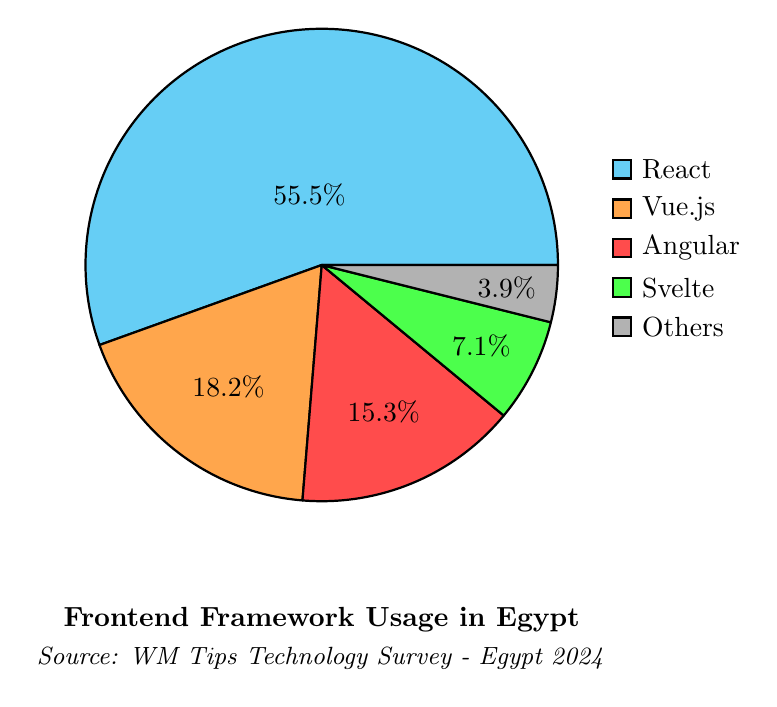
\begin{tikzpicture}
    \pie[
        radius=3,
        text=legend,
        color={cyan!60, orange!70, red!70, green!70, gray!60}
    ]{
        55.5/React,
        18.2/Vue.js,
        15.3/Angular,
        7.1/Svelte,
        3.9/Others
    }
    \node at (0, -4.5) {\textbf{Frontend Framework Usage in Egypt}};
    \node at (0, -5) {\small\textit{Source: WM Tips Technology Survey - Egypt 2024}};
\end{tikzpicture}
\caption{Frontend Framework Market Share in Egypt}
\end{figure}

React's dominant 55.5\% market share in Egypt significantly exceeds its global average of 40.6\%, demonstrating strong regional alignment with our technology selection.

\subsubsection{React Ecosystem Strength}

The React ecosystem provides unparalleled support infrastructure:

\begin{figure}[H]
\centering
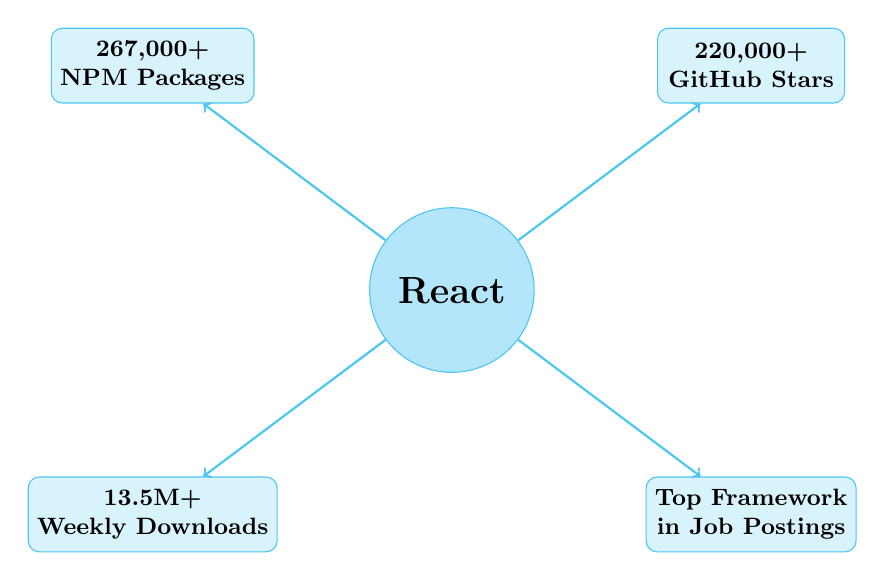
\begin{tikzpicture}[scale=0.95, every node/.style={scale=0.95}]
    % Central node
    \node[circle, draw=cyan!70, fill=cyan!30, minimum size=2.2cm, font=\Large\bfseries, align=center] (react) at (0,0) {React};
    
    % Surrounding ecosystem
    \node[rectangle, rounded corners, draw=cyan!70, fill=cyan!15, minimum width=2.5cm, minimum height=1cm, font=\small\bfseries, align=center] (npm) at (-4, 3) {267,000+\\NPM Packages};
    
    \node[rectangle, rounded corners, draw=cyan!70, fill=cyan!15, minimum width=2.5cm, minimum height=1cm, font=\small\bfseries, align=center] (github) at (4, 3) {220,000+\\GitHub Stars};
    
    \node[rectangle, rounded corners, draw=cyan!70, fill=cyan!15, minimum width=2.5cm, minimum height=1cm, font=\small\bfseries, align=center] (community) at (-4, -3) {13.5M+\\Weekly Downloads};
    
    \node[rectangle, rounded corners, draw=cyan!70, fill=cyan!15, minimum width=2.5cm, minimum height=1cm, font=\small\bfseries, align=center] (jobs) at (4, -3) {Top Framework\\in Job Postings};
    
    \draw[thick, ->, cyan!70] (react) -- (npm);
    \draw[thick, ->, cyan!70] (react) -- (github);
    \draw[thick, ->, cyan!70] (react) -- (community);
    \draw[thick, ->, cyan!70] (react) -- (jobs);
\end{tikzpicture}
\caption{React Ecosystem Metrics}
\end{figure}

\vspace{0.3cm}
\textit{Source: NPM Statistics 2025, GitHub Octoverse 2024}

\subsection{Conclusion}

The zGate Admin Panel WebUI represents a successful synthesis of modern web development practices and enterprise security requirements. By leveraging industry-leading technologies (React, Next.js, TypeScript) backed by compelling market data, the interface delivers both exceptional user experience and robust security controls. The technology stack's strong adoption trends, combined with high developer satisfaction scores, position zGate for long-term maintainability and scalability. As demonstrated by the market analysis, our technology choices align with both global standards and regional Egyptian market dynamics, ensuring talent availability and industry relevance for years to come.

% ============================================================
% 13. TECHNOLOGY JUSTIFICATION
% ============================================================
\chapter{Technology Justification}

\section{Why Go}
The selection of Go (Golang) as the primary language for implementing the zGate Gateway proxy was driven by several technical requirements unique to high-performance, security-critical network infrastructure. Unlike interpreted languages, Go provides the performance characteristics and concurrency model essential for building a production-grade database access proxy.

\subsection{Performance \& Execution Model}
Go is a compiled language that translates source code directly into machine code, unlike interpreted languages such as Python that execute code line-by-line at runtime. This fundamental architectural difference results in significantly lower latency and higher throughput—critical metrics for a proxy that sits between clients and database servers, where every millisecond of added latency compounds across thousands of queries.

Additionally, Go applications exhibit substantially lower memory overhead compared to equivalent implementations in interpreted languages. This efficiency allows the gateway to handle significantly more concurrent traffic on the same hardware resources, directly impacting the scalability and cost-effectiveness of the system.

\subsection{Goroutine Concurrency Model}
The most significant advantage of Go for proxy server implementation lies in its concurrency model based on goroutines. This feature is crucial for handling the massive number of simultaneous database connections that a production gateway must support.

Traditional threading models impose significant memory overhead, as each thread typically consumes megabytes of stack space. In contrast, goroutines are extremely lightweight, consuming only approximately 2KB of initial stack space. This efficiency enables the gateway to spawn tens of thousands of goroutines to handle concurrent proxy connections without exhausting system resources—a capability that would be impractical with traditional threading approaches.

Furthermore, Go provides \textit{channels} as a first-class language construct for safely communicating between concurrent processes. This built-in mechanism eliminates the complex locking patterns and race conditions that plague concurrent programming in other languages, making the codebase more maintainable and less prone to subtle concurrency bugs.

\subsection{Production-Grade Standard Library}
Go was designed by Google specifically for building networked systems and internet services. The standard library's \texttt{net} and \texttt{net/http} packages are robust, secure, and production-ready out of the box, eliminating the need for heavy external frameworks.

The \texttt{net} library provides fine-grained control over TCP socket behavior, including precise management of timeouts, deadlines, and keep-alive settings. This low-level control is essential for a custom proxy that must intelligently manage traffic flow, implement connection pooling, and enforce session policies at the transport layer.

\subsection{Security \& Cryptography Ecosystem}
Security is paramount for a Zero Trust database access gateway, and Go's cryptography ecosystem is exceptionally well-suited to this requirement. The \texttt{crypto/tls} package in Go is considered one of the industry's best implementations of SSL/TLS protocols, with built-in support for modern standards including TLS 1.3 by default.

Critically, Go is a memory-safe language despite its performance characteristics comparable to C or C++. The language's garbage collector prevents common security vulnerabilities such as buffer overflows, use-after-free errors, and memory leaks—all of which would be catastrophic in a security gateway positioned between untrusted clients and sensitive database systems.

\subsection{Deployment Simplicity}
Go's compilation model produces a single static binary that bundles all dependencies and libraries. This characteristic eliminates "dependency hell" and dramatically simplifies deployment operations.

To deploy the zGate Gateway to a server or container, operators simply copy a single executable file—no runtime installation, no package manager invocations, and no version conflict resolution required. This simplicity reduces the attack surface, minimizes deployment complexity, and ensures consistent behavior across different target environments.

\subsection{Developer Experience \& Code Maintainability}
Go's minimalist design philosophy emphasizes simplicity and readability, featuring a deliberately small syntax with no complex inheritance hierarchies or implicit behaviors. This characteristic is particularly valuable for security-critical software, where code auditability is essential. If code is easy to read, it is correspondingly easier to audit for security flaws and verify correctness.

As a statically typed language with a powerful type system, Go enables the compiler to catch many classes of bugs—including type mismatches, null pointer dereferences, and interface violations—before code execution. This compile-time validation substantially reduces the likelihood of runtime errors in production environments, contributing to overall system reliability.

\section{Why Node.js / TS / React}

\section{Why SQLite for Internal Storage}
The evolution of the zGate Gateway's configuration management architecture represents a critical design decision that directly impacts system reliability, security, and operational efficiency. Initially, the system utilized YAML files for storing configuration data, including database connection strings, user permissions, and policy rules. However, this approach proved insufficient for a production-grade security gateway, leading to the adoption of SQLite as the internal storage mechanism.

\subsection{Zero-Downtime Updates}
The most significant limitation of file-based configuration was the requirement for application restarts to apply changes. In the YAML-based implementation, configuration data was loaded into memory only during application startup. Any modification to proxy rules, database connection strings, or user permissions required editing the file and restarting the entire gateway—an operation that necessarily resulted in dropped connections and service interruption.

SQLite fundamentally resolves this issue by enabling real-time configuration queries. When an administrator updates a setting through the WebUI, the change is committed to the database immediately and atomically. Subsequent requests automatically retrieve the updated configuration without requiring any application restart or service disruption. This capability is essential for maintaining high availability in production environments where configuration changes are routine operational tasks.

\subsection{Efficiency \& Memory Management}
The YAML approach required loading the entire configuration dataset into memory at startup, creating a cached representation of all configuration data. This architecture introduced several problems, including memory inefficiency and the risk of state drift—a condition where in-memory data diverges from the on-disk representation if files are modified externally or by concurrent processes.

SQLite's relational model eliminates these issues through structured, on-demand data access. Rather than maintaining complex nested maps and arrays in memory, the gateway queries specific configuration elements exactly when needed. This approach significantly reduces the application's memory footprint, particularly as the configuration dataset grows to encompass hundreds of database connections, thousands of user accounts, and complex policy rules.

Furthermore, SQLite's query optimizer ensures that data retrieval operations are efficient even as the dataset scales, something that would require substantial custom indexing logic if implemented with in-memory data structures.

\subsection{API Integration \& WebUI Compatibility}
Modern administrative interfaces require comprehensive Create, Read, Update, and Delete (CRUD) operations on configuration data. Implementing these operations safely with YAML files—particularly handling concurrent modifications, maintaining data integrity, and providing transactional semantics—is complex and error-prone.

SQLite provides a standardized SQL interface that dramatically simplifies API development. The Go backend can leverage SQL's powerful query capabilities to implement sophisticated operations with minimal code. For example, filtering connection strings by environment, paginating audit logs, or searching for users by role becomes trivial with SQL queries:

\begin{verbatim}
SELECT * FROM connections 
WHERE environment='production' 
ORDER BY name LIMIT 10
\end{verbatim}

This SQL-based approach integrates seamlessly with the React/Node.js WebUI, which can issue standard REST API calls that translate directly to SQL queries. The result is a clean, maintainable codebase with clear separation between the presentation layer (React), business logic (Node.js API), and data persistence (SQLite).

\subsection{Enhanced Security Through Data-at-Rest Encryption}
Security considerations provided the final compelling argument for SQLite adoption. YAML files are inherently plain text, meaning that any attacker who gains read access to the server's filesystem can immediately view all sensitive configuration data, including database credentials, encryption keys, and access tokens.

To address this vulnerability, the gateway implements a data-at-rest encryption strategy using AES (Advanced Encryption Standard). Before persisting sensitive data to the SQLite database, the Go application encrypts it using AES-256 in GCM mode. Database connection strings, API keys, and other sensitive fields are stored only in their encrypted form.

The practical impact of this approach is substantial: even if an attacker obtains a copy of the SQLite database file through a filesystem breach or backup compromise, the sensitive columns contain only cryptographically secure ciphertext. Only the running Go application, which holds the master encryption key in memory (and never persists it to disk), can decrypt and utilize the actual configuration data. This defense-in-depth strategy aligns with Zero Trust principles by assuming that filesystem access controls may be breached and providing an additional layer of protection.

\section{Why mTLS (and why TCP is temporary)}
\section{Design Decision Summary}

% ============================================================
% 14. PROTOTYPE – SEMESTER 1
% ============================================================
\chapter{Prototype – Semester 1}
\section{Implemented Features}
\section{Screenshots (CLI \& Dashboard)}
\section{What Works vs What Doesn't}
\section{Technical Decisions Made}
\section{Implementation Challenges}

% ============================================================
% 15. DEVELOPMENT METHODOLOGY
% ============================================================

\begin{sectionintro}{15}{Development Methodology}{
  \begin{itemize}[leftmargin=1.5em]
    \item Agile Scrum framework implementation
    \item Sprint planning and iteration cycles
    \item Meeting structure and collaboration patterns
    \item Development tools and workflows
    \item Quality assurance processes
  \end{itemize}
}
\lettrine[lines=3, lhang=0.1, loversize=0.2]{\color{primaryBlue}M}{ethodology determines how effectively a team transforms requirements into working software.} This chapter describes the Agile Scrum framework adopted for zGate development, including sprint structures, meeting cadences, and collaborative workflows. The methodology emphasizes rapid iteration, continuous feedback, and systematic progress tracking to ensure alignment with project objectives.
\end{sectionintro}

\section{Agile Scrum Framework}
To manage the complexity of the project and ensure continuous development, the team adopted the Agile Scrum methodology. We structured the development lifecycle into one-week sprints, enabling rapid iteration and frequent feedback cycles. This short sprint duration allowed us to demonstrate tangible progress weekly and incorporate supervisor feedback more frequently, ensuring alignment with project objectives throughout the development process.

\section{Meeting Structure}
Our workflow is organized around three distinct meeting types: the Weekly Kick-off, Daily Stand-ups, and the Sprint Review with stakeholders. This structured rhythm of recurring meetings ensures that team milestones and progress are consistently monitored and synchronized. Collectively, these meetings serve to define, review, and align all weekly tasks in accordance with agile best practices.

\subsection{Weekly Kick-off Meeting}
This meeting is held at the start of every sprint to align the team for the upcoming week. It encompasses three key components:
\begin{itemize}
    \item \textbf{Retrospective:} We briefly analyze the previous sprint, discussing what went well and identifying bottlenecks (e.g., merge conflicts or unclear requirements). This reflection helps the team avoid repeating past mistakes and continuously improve our process.
    \item \textbf{Backlog Refinement:} We review upcoming tasks to ensure they are clearly defined and that all technical requirements are understood before assignment. This step reduces ambiguity and sets clear expectations.
    \item \textbf{Sprint Planning:} We select specific tasks from the refined backlog to be completed in the current week. Tasks are assigned to team members based on priority, complexity, and estimated effort.
\end{itemize}

\subsection{Daily Stand-up Meeting}
This brief synchronization meeting is held daily to maintain continuous team alignment and identify blockers early.
\begin{itemize}
    \item \textbf{Duration:} Limited to approximately 15 minutes total, with each member speaking for no more than 2 minutes. This time constraint ensures the meeting remains focused and efficient.
    \item \textbf{Format:} Each team member addresses two specific points: what they accomplished yesterday and what they plan to work on today. Any blockers or dependencies are also raised.
    \item \textbf{Objective:} This practice ensures that no team member works in isolation or is blocked by dependencies without the rest of the team being aware. It promotes transparency and enables rapid problem-solving.
\end{itemize}

\subsection{Sprint Review (Weekly Supervisor Meeting)}
At the conclusion of each sprint, a formal review is conducted with our project supervisor and mentors to validate progress and gather feedback.
\begin{itemize}
    \item \textbf{Demonstration:} The team presents the functional features completed during the sprint, showcasing working software rather than just documentation or plans.
    \item \textbf{Validation:} Our supervisors provide immediate feedback on the implementation. This feedback is either approved for integration or converted into new change requests to be prioritized in the next sprint's backlog.
\end{itemize}

\section{Collaboration Tools}
To ensure accessibility and efficient collaboration across all phases of development, we employ an integrated tool stack that supports both synchronous and asynchronous communication:
\begin{description}
    \item[Central Knowledge Base (Notion):] Serves as the single source of truth for the project wiki. It is used for sprint planning, task and goal tracking, documenting new code features, and archiving meeting notes and recordings. All team members have real-time access to project documentation.
    \item[Version Control \& Technical Documentation (GitHub):] The primary repository for source code, version control, and code reviews. GitHub also hosts technical documentation, including the Proxy Installation Guide and API references.
    \item[Synchronous Communication:] Discord, Microsoft Teams, and Google Meet are used for scheduled meetings and real-time voice/video collaboration. These platforms facilitate immediate discussion and decision-making.
    \item[Asynchronous Communication:] WhatsApp is used for quick, urgent team notifications and simple coordination when immediate responses are needed outside of scheduled meetings.
    \item[Auxiliary Tools:] We leverage AI-powered tools for generating meeting summaries and conclusions, creating immediate and searchable records of discussions. Excalidraw is used for creating collaborative diagrams, flowcharts, and architectural drawings during design discussions.
\end{description}

\section{Documentation \& Observability}
We prioritize high observability by documenting all progress, regardless of scale. This comprehensive documentation approach ensures transparency and facilitates knowledge transfer within the team.

While day-to-day execution is tracked in Notion, high-level progress reporting is documented in a formal \textbf{Supervisor Meeting Log} maintained as a Word document. This log serves as an official record and tracks:
\begin{itemize}
    \item \textbf{Attendance \& Date:} A record of meeting participants and timestamps.
    \item \textbf{Retrospective:} Feedback on completed tasks, including what was delivered and any deviations from the plan.
    \item \textbf{Forward Planning:} Clearly defined goals and expected outcomes for the subsequent meeting, establishing accountability and measurable targets.
\end{itemize}

% ============================================================
% 17. MILESTONES
% ============================================================
\chapter{Milestones}
\section{Term 1 Milestone Roadmap}
\subsection{Milestone 1}
\subsection{Milestone 2}
\subsection{Milestone 3}
\subsection{Milestone 4}
\subsection{Milestone 5}
\section{Timeline Chart (Gantt-like)}

% ============================================================
% PROJECT RISK MANAGEMENT
% ============================================================

\begin{sectionintro}{18}{Project Risk Management}{
  \begin{itemize}[leftmargin=1.5em]
    \item Protocol engineering complexity
    \item Performance and latency optimization
    \item Security implementation challenges
    \item Database compatibility issues
    \item Scope and schedule management
    \item Team skill development
  \end{itemize}
}
\lettrine[lines=3, lhang=0, loversize=0.15]{\color{primaryBlue}R}{isk management is critical for engineering complex security systems.} This chapter analyzes potential risks including protocol reverse engineering complexity, performance optimization challenges, TLS implementation security, database driver compatibility issues, scope creep, and team skill development. We establish mitigation strategies for each identified risk and define a dynamic monitoring framework to ensure successful delivery.
\end{sectionintro}

\section{Introduction}
\IEEEPARstart{T}{he} development of a high-performance, security-critical infrastructure component such as the zGate Database Proxy involves a multitude of complex challenges that extend beyond simple implementation details. Effective risk management is therefore not merely an ancillary activity but a core pillar of our engineering methodology. This chapter provides a comprehensive analysis of the potential risks identified throughout the project lifecycle, categorized into technical, operational, and schedule-based domains. By proactively identifying these risks, establishing their probability and impact, and formulating robust mitigation strategies, the development team aims to minimize uncertainty and ensure the successful delivery of a production-grade Zero Trust solution.

Our risk management framework is dynamic; it is designed to be revisited during each sprint retrospective to ensure that new risks are captured and that the status of existing risks is updated as mitigation strategies are executed.

\section{Risk Assessment Methodology}

To quantify and prioritize risks effectively, we have adopted a standard Risk Assessment Matrix approach. This methodology evaluates each identified risk along two primary dimensions:

\begin{enumerate}
    \item \textbf{Likelihood:} The probability that the risk event will materialize.
    \item \textbf{Impact:} The severity of the consequences should the risk operationalize.
\end{enumerate}

Based on these two factors, we classify risks into three tiers:
\begin{itemize}
    \item \textbf{Critical Risk:} Requires immediate attention and the development of a detailed contingency plan. These risks have the potential to halt project progress or cause total system failure.
    \item \textbf{High Risk:} Significant threats that require active monitoring and specific mitigation tasks to be integrated into the development backlog.
    \item \textbf{Medium/Low Risk:} Risks that are monitored periodically but do not strictly dictate immediate changes to the project roadmap.
\end{itemize}

\begin{table}[h]
\centering
\renewcommand{\arraystretch}{1.5}
\resizebox{\textwidth}{!}{%
\begin{tabular}{|l|c|c|c|}
\hline
\textbf{Risk Description} & \textbf{Likelihood} & \textbf{Impact} & \textbf{Risk Level} \\
\hline
Reverse Engineering Complexity (Undocumented Protocols) & High & High & \textbf{Critical} \\
\hline
Performance/Latency Overhead Exceeding Budget & Medium & High & \textbf{High} \\
\hline
Security Vulnerabilities in Proxy Implementation & Low & Critical & \textbf{High} \\
\hline
Third-Party SSO Integration Incompatibility & Medium & Medium & \textbf{Medium} \\
\hline
Scope Creep (Feature Overload) & High & Medium & \textbf{High} \\
\hline
Team Skill Acquisition Curve (Go/Systems Programming) & Low & High & \textbf{Medium} \\
\hline
\end{tabular}%
}
\caption{Detailed Project Risk Assessment Matrix}
\label{tab:risk-matrix}
\end{table}

\section{Technical Risks Analysis}

Technical risks represent the most significant threat to the project's success, primarily due to the low-level nature of the work involving binary protocols and network systems.

\subsection{Protocol Reverse Engineering and Parsing Complexity}
\textbf{Description:}
The core function of zGate relies on the ability to flawlessly intercept, parse, and reconstruct binary wire protocols (MySQL Client/Server Protocol and Microsoft SQL Server TDS). These protocols are often proprietary (in the case of TDS) or complexly versioned. There is a significant risk that undocumented behaviors, specific flag combinations, or version discrepancies could cause the proxy to misinterpret packet boundaries.

\textbf{Potential Consequences:}
\begin{itemize}
    \item \textbf{Data Corruption:} Incorrectly reconstructing a packet could corrupt the SQL query or the result set returning to the client.
    \item \textbf{Connection Instability:} If the proxy fails to respond to a "Heartbeat" or "Ping" packet correctly due to parsing errors, the database client may terminate the connection.
    \item \textbf{Vendor Lock-in:} The implementation might inadvertently become too coupled to a specific version of MySQL or MSSQL, failing when the database server is patched or upgraded.
\end{itemize}

\textbf{Mitigation Strategy:}
To mitigate this critical risk, the team is employing a "Defense in Depth" strategy for parsing:
\begin{itemize}
    \item \textbf{Granular Unit Testing:} We implement unit tests for every packet type using captured bytes from real production traffic (using Wireshark) to ensure byte-for-byte accuracy.
    \item \textbf{Fuzz Testing:} We plan to use Go's fuzzing capabilities to send random garbage data to the parsers to ensure they handle errors gracefully without crashing the entire service.
    \item \textbf{Opaque Forwarding Fallback:} For parts of the protocol that are not strictly relevant to security policy (e.g., obscure handshake flags), the proxy is designed to forward bytes transparently rather than attempting to parse and re-serialize them, reducing the surface area for errors.
\end{itemize}

\subsection{Performance and Latency Overhead}
\textbf{Description:}
By introducing a "Man-in-the-Middle" proxy between the application and the database, we inevitably introduce network latency. This includes the time taken for TCP socket reads, context switching in the Operating System, memory allocation for packet buffers, and the logic execution time of the Policy Engine.

\textbf{Potential Consequences:}
If the added latency exceeds a threshold of approximately 10-20ms per query, the solution may be deemed unusable for high-frequency trading platforms or real-time applications, leading to rejection by stakeholders.

\textbf{Mitigation Strategy:}
\begin{itemize}
    \item \textbf{Zero-Copy Networking:} We leverage Go's \texttt{io.Reader} and \texttt{io.Writer} interfaces to stream data efficiently, aiming to minimize user-space memory copying.
    \item \textbf{Concurrency Model:} Utilizing Go's lightweight goroutines ensures that handling thousands of concurrent connections does not incur the heavy memory and CPU context-switching penalties associated with traditional thread-per-connection models (like Java or C++ threads).
    \item \textbf{Profiling and Benchmarking:} Regular performance profiling using `pprof` is conducted during the development cycle (not just at the end) to identify "hot paths" in the code and optimize them immediately.
\end{itemize}

\subsection{TLS and Cryptographic Handshake Failures}
\textbf{Description:}
As a security proxy, zGate must terminate TLS connections from clients and establish new TLS connections to backend databases. This introduces a "Man-in-the-Middle" architecture where certificate validation, cipher suite negotiation, and protocol versions (TLS 1.2 vs 1.3) must be handled perfectly. The risk is that strict client drivers may reject the proxy's self-signed or internal CA-signed certificates, or that the proxy fails to negotiate a common cipher suite with legacy databases.

\textbf{Potential Consequences:}
\begin{itemize}
    \item \textbf{Connectivity Blockers:} Modern drivers (e.g., latest JDBC) often default to "Strict" SSL modes. If the proxy's TLS implementation is flawed, these clients will refuse to connect entirely.
    \item \textbf{Security Degradation:} A misconfiguration could inadvertently downgrade connections to plaintext or weak ciphers, violating the very Zero Trust principles the project aims to uphold.
\end{itemize}

\textbf{Mitigation Strategy:}
\begin{itemize}
    \item \textbf{Standard Library Usage:} We rely strictly on Go's `crypto/tls` standard library rather than rolling custom crypto code, ensuring compliance with modern standards.
    \item \textbf{Configurable CA Trust:} The proxy is designed to allow easy injection of root CA certificates into client trust stores (via the CLI) to facilitate smooth "internal" certificate validation.
\end{itemize}

\subsection{Database Driver Compatibility}
\textbf{Description:}
Not all database clients are created equal. While the `mysql` CLI might behave one way, the MySQL driver for Python (PyMySQL), Java (Connector/J), or Go (go-sql-driver) may use slightly different subsets of the wire protocol or rely on specific "undocumented" behavior (e.g., specific expecting order of handshake packets).

\textbf{Potential Consequences:}
The proxy might work perfectly for one set of tools but fail catastrophically for another, severely limiting its adoption.

\textbf{Mitigation Strategy:}
\begin{itemize}
    \item \textbf{Broad Integration Testing:} Our test suite includes "Smoke Tests" that connect to the proxy using a variety of real-world drivers (Python, Node.js, Java) to verify cross-platform compatibility.
\end{itemize}

\subsection{SQL Parsing and AST Limitations}
\textbf{Description:}
To enforce fine-grained policies (e.g., "User X cannot query Table Y"), zGate must parse incoming SQL strings into an Abstract Syntax Tree (AST). SQL is a complex, context-sensitive language with many proprietary extensions. There is a risk that our parser implementation may fail to understand complex nested queries, CTEs (Common Table Expressions), or stored procedure calls.

\textbf{Potential Consequences:}
\begin{itemize}
    \item \textbf{False Positives/Negatives:} The Policy Engine might block a legitimate query because it poorly understands the syntax, or worse, allow a malicious query because it failed to detect a forbidden object access hidden in a subquery.
\end{itemize}

\textbf{Mitigation Strategy:}
\begin{itemize}
    \item \textbf{Library Adoption:} Instead of writing a parser from scratch, we utilize battle-tested open-source SQL parsers (like `pingcap/tidb/parser` for MySQL) that are already used in production databases. This significantly reduces the risk of parsing errors compared to a home-grown solution.
\end{itemize}

\section{Operational and Project Management Risks}

Beyond the technical challenges, the project faces operational risks related to scope, resources, and timeline.

\subsection{Scope Creep and Feature Bloat}
\textbf{Description:}
The domain of Zero Trust security is vast. There is a constant temptation to add "just one more feature," such as AI-based anomaly detection, support for PostgreSQL/Oracle/MongoDB, or complex User Behavior Analytics (UBA).

\textbf{Potential Consequences:}
Attempting to implement too many features simultaneously risks diluting the team's focus, resulting in a system where many features are "half-done" but nothing is production-ready. This constitutes a classic software engineering failure mode known as "Gold Plating."

\textbf{Mitigation Strategy:}
\begin{itemize}
    \item \textbf{Strict Prioritization:} We strictly adhere to the MoSCoW method (Must have, Should have, Could have, Won't have). Milestone 3 (POC) and Milestone 4 (SSO) are "Must Haves."
    \item \textbf{Agile Iterations:} The two-week sprint cycle forces the team to deliver shippable increments. If a feature cannot be completed in a sprint, it is re-evaluated.
    \item \textbf{Supervisor Alignment:} Regular syncs with project supervisors ensure that the scope remains realistic and aligned with academic requirements rather than commercial ambitions.
\end{itemize}

\subsection{Team Skill Gaps and Technology Adoption}
\textbf{Description:}
The technology stack for zGate includes Systems Programming (Go), Frontend Development (React/TypeScript), and Cryptography concepts. It is rare for all team members to be equally proficient in all these areas.

\textbf{Potential Consequences:}
A "knowledge silo" effect may occur where only one person understands the core proxy code, creating a "Bus Factor" of 1. If that team member becomes unavailable, the project stalls.

\textbf{Mitigation Strategy:}
\begin{itemize}
    \item \textbf{Code Reviews:} All pull requests require review by at least one other team member. This forces knowledge sharing and ensures that code is readable and maintainable by others.
    \item \textbf{Pair Programming:} For the most complex components (like the TDS protocol implementations), we utilize pair programming to solve problems collaboratively and level up skills in real-time.
    \item \textbf{Dedicated Research Phase:} Milestone 2 was explicitly dedicated to skill acquisition, ensuring the team had a foundation before writing production code.
\end{itemize}

\section{Contingency Planning}
Despite rigorous planning, unforeseen issues ("Unknown Unknowns") can arise. To account for this, the roadmap for Term 2 includes a specific "stabilization buffer" of two weeks around Milestone 6.

If critical technical blockers arise that jeopardize the final delivery date—for example, if the MSSQL encryption handshake proves resistant to interception—the team has agreed on a "Scope Reduction Protocol." Under this protocol, we would pivot to focusing exclusively on perfecting the MySQL implementation to a commercial standard, rather than delivering a flawed multi-database support. This ensures that the final deliverable, while potentially smaller in scope, remains high-quality and fully functional.

% ============================================================
% 19. ROADMAP FOR TERM 2
% ============================================================
\chapter{Roadmap for Term 2}

Term~2 represents the critical transition from a functional Proof of Concept to a production-ready database security solution. Building upon the foundational work completed in Term~1, the development team will focus on three primary areas: integrating enterprise-grade identity management, implementing comprehensive observability features, and conducting rigorous validation to ensure system reliability and security.

\section{Remaining Features}

The following features are scheduled for implementation during Term~2, organized by milestone and priority.

\subsection{External Identity Provider Integration (Milestone 4)}

The current POC utilizes an internal token-based authentication system. Term~2 will extend this to support federated identity management through external providers.

\begin{itemize}
    \item \textbf{OAuth2/OIDC Implementation:} Integrate industry-standard authentication protocols to enable Single Sign-On (SSO) capabilities.
    \item \textbf{Identity Provider Support:} Configure connectors for major identity providers including:
    \begin{itemize}
        \item Google Workspace
        \item Microsoft Azure Active Directory
        \item Okta
        \item Generic SAML 2.0 providers
    \end{itemize}
    \item \textbf{Claims-to-Role Mapping:} Develop a flexible mapping engine that translates IdP claims (groups, roles, attributes) to zGate's internal RBAC policies.
    \item \textbf{Just-in-Time Provisioning:} Implement automatic user provisioning based on IdP attributes upon first login.
\end{itemize}

\subsection{Enhanced Observability Features (Milestone 5)}

Transform the initial dashboard into a comprehensive monitoring and compliance platform.

\begin{itemize}
    \item \textbf{Real-Time Metrics Dashboard:}
    \begin{itemize}
        \item Connection pool utilization graphs
        \item Query throughput and latency percentiles
        \item Active session monitoring
        \item Database health indicators
    \end{itemize}
    \item \textbf{Audit Logging System:}
    \begin{itemize}
        \item Structured logging of all database access events
        \item Query content capture with optional redaction
        \item User activity timeline visualization
        \item Export capabilities for compliance reporting (CSV, JSON, SIEM integration)
    \end{itemize}
    \item \textbf{Alerting Framework:}
    \begin{itemize}
        \item Configurable threshold-based alerts
        \item Anomaly detection for unusual access patterns
        \item Integration with notification channels (email, Slack, webhooks)
    \end{itemize}
\end{itemize}

\subsection{Advanced Policy Engine Enhancements}

Extend the current policy engine with more granular control mechanisms.

\begin{itemize}
    \item \textbf{Time-Based Access Controls:} Implement policies that restrict database access to specific time windows.
    \item \textbf{Query Complexity Limits:} Add configurable limits on query complexity to prevent resource exhaustion.
    \item \textbf{Row-Level Security Policies:} Develop mechanisms to enforce row-level filtering based on user identity.
    \item \textbf{Dynamic Masking Rules:} Extend data masking to support context-aware redaction based on user roles.
\end{itemize}

%-----------------------------------------------------------

\section{Architecture Improvements}

Based on lessons learned during POC development, the following architectural enhancements are planned.

\subsection{Scalability Enhancements}

\begin{itemize}
    \item \textbf{Horizontal Scaling Support:} Implement stateless proxy instances that can be load-balanced for high availability.
    \item \textbf{Connection Multiplexing:} Optimize connection pooling to support higher concurrent user loads with fewer backend connections.
    \item \textbf{Caching Layer:} Introduce caching for policy decisions and session metadata to reduce latency.
\end{itemize}

\subsection{Security Hardening}

\begin{itemize}
    \item \textbf{TLS Certificate Management:} Implement automated certificate rotation and enhanced certificate validation.
    \item \textbf{Secret Management Integration:} Support for external secret stores (HashiCorp Vault, AWS Secrets Manager).
    \item \textbf{Audit Trail Integrity:} Implement cryptographic signing of audit logs to ensure tamper-evidence.
\end{itemize}

\subsection{Deployment Improvements}

\begin{itemize}
    \item \textbf{Container Orchestration:} Official Docker images and Kubernetes Helm charts for production deployment.
    \item \textbf{Configuration Management:} Migration to environment-based configuration with validation on startup.
    \item \textbf{Health Check Endpoints:} Enhanced liveness and readiness probes for orchestrator integration.
\end{itemize}

%-----------------------------------------------------------

\section{Performance Goals}

Table~\ref{tab:performance-goals} outlines the target performance metrics for the production release.

\begin{table}[htbp]
\centering
\caption{Term 2 Performance Targets}
\label{tab:performance-goals}
\begin{tabular}{|l|l|l|}
\hline
\textbf{Metric} & \textbf{Target} & \textbf{Measurement Method} \\
\hline
Latency Overhead (p50) & $<$ 2ms & Benchmarking with synthetic load \\
Latency Overhead (p99) & $<$ 10ms & Benchmarking under stress \\
Concurrent Connections & $\geq$ 1000 & Load testing with connection ramp \\
Connection Setup Time & $<$ 50ms & End-to-end connection timing \\
Memory Footprint & $<$ 500MB (idle) & Resource monitoring under load \\
CPU Utilization & $<$ 30\% (normal load) & Profiling during benchmark \\
\hline
\end{tabular}
\end{table}

\subsection{Optimization Strategies}

To achieve these performance targets, the following optimization strategies will be employed:

\begin{enumerate}
    \item \textbf{Profiling-Driven Optimization:} Use Go's built-in profiler (pprof) to identify and eliminate bottlenecks.
    \item \textbf{Memory Pool Management:} Implement buffer pooling to reduce garbage collection overhead.
    \item \textbf{Protocol Parser Optimization:} Optimize hot paths in protocol parsing using zero-copy techniques where applicable.
    \item \textbf{Goroutine Pool Management:} Implement worker pools to prevent goroutine explosion under high load.
\end{enumerate}

%-----------------------------------------------------------

\section{Testing \& Validation Plan}

A comprehensive testing strategy will ensure system reliability and security before final delivery.

\subsection{Automated Testing Framework}

\begin{itemize}
    \item \textbf{Unit Tests:} Target minimum 80\% code coverage for core proxy logic and security modules.
    \item \textbf{Integration Tests:} End-to-end tests covering authentication flows, query processing, and data masking across all supported databases.
    \item \textbf{Regression Test Suite:} Automated test suite executed on every code commit via CI/CD pipeline.
\end{itemize}

\subsection{Performance Validation}

\begin{itemize}
    \item \textbf{Load Testing:} Use tools such as \texttt{pgbench} (PostgreSQL), \texttt{mysqlslap} (MySQL), and custom scripts to simulate production workloads.
    \item \textbf{Stress Testing:} Evaluate system behavior under extreme conditions (connection floods, memory pressure).
    \item \textbf{Latency Profiling:} Measure and document latency distribution across different query types and database backends.
\end{itemize}

\subsection{Security Validation}

\begin{itemize}
    \item \textbf{Penetration Testing:} Internal security audit focusing on:
    \begin{itemize}
        \item SQL injection bypass attempts
        \item Authentication bypass vectors
        \item Token forging and replay attacks
        \item Policy engine circumvention
    \end{itemize}
    \item \textbf{Threat Modeling:} Document potential attack vectors and corresponding mitigations.
    \item \textbf{Dependency Audit:} Scan all dependencies for known vulnerabilities using automated tools.
\end{itemize}

\subsection{User Acceptance Testing}

\begin{itemize}
    \item \textbf{Supervisor Demonstrations:} Weekly demonstrations of new features to project supervisors.
    \item \textbf{Documentation Review:} Validation that all user-facing documentation accurately reflects system behavior.
    \item \textbf{Demo Environment:} Prepare a stable demonstration environment for final presentation.
\end{itemize}

\subsection{Validation Timeline}

Table~\ref{tab:testing-timeline} presents the planned testing phases and their timelines.

\begin{table}[htbp]
\centering
\caption{Testing \& Validation Timeline}
\label{tab:testing-timeline}
\begin{tabular}{|l|l|l|}
\hline
\textbf{Testing Phase} & \textbf{Timeline} & \textbf{Focus Area} \\
\hline
Unit \& Integration Testing & Ongoing (all sprints) & Continuous quality assurance \\
Performance Benchmarking & May 1--15 & Latency and throughput validation \\
Security Audit & May 15--31 & Penetration testing and hardening \\
User Acceptance Testing & June 1--10 & Feature validation and feedback \\
Final Documentation Review & June 10--15 & Documentation completeness \\
Demo Environment Preparation & June 15--20 & Final presentation preparation \\
\hline
\end{tabular}
\end{table}

%-----------------------------------------------------------

%\section{Term 2 Development Timeline}

%The following Mermaid diagram can be used to visualize the Term~2 development timeline:

% Mermaid Syntax for Term 2 Gantt Chart:
% 
% gantt
%     title zGate Term 2 Development Timeline
%     dateFormat  YYYY-MM-DD
%     axisFormat  %b %d
%     
%     section Milestone 4: IAM Integration
%     OAuth2/OIDC Implementation     :m4a, 2025-01-15, 21d
%     IdP Connectors (Google, Okta)  :m4b, after m4a, 14d
%     Claims-to-Role Mapping         :m4c, after m4b, 14d
%     
%     section Milestone 5: Observability
%     Metrics Dashboard              :m5a, 2025-03-01, 21d
%     Audit Logging System           :m5b, after m5a, 21d
%     Alerting Framework             :m5c, after m5b, 14d
%     
%     section Milestone 6: Validation
%     Performance Benchmarking       :m6a, 2025-05-01, 14d
%     Security Audit                 :m6b, after m6a, 14d
%     Final Documentation            :m6c, 2025-05-15, 30d
%     Demo Preparation               :m6d, 2025-06-10, 10d

% Note: Generate this diagram using a Mermaid renderer and include as figure

% ============================================================
% 20. TEAM CONTRIBUTION
% ============================================================
\chapter{Team Contribution}

This chapter documents the individual contributions of each team member throughout the development of the zGate Zero-Trust Database Access Gateway. The project required expertise across multiple domains including backend systems programming, frontend development, security engineering, and research.

\section{Overview of Contribution Approach}

The zGate project was developed by a seven-member team, with responsibilities distributed across the following primary domains:

\begin{itemize}
    \item \textbf{Backend \& Proxy Development:} Core proxy logic, protocol handlers, connection management
    \item \textbf{Security Engineering:} Authentication, authorization, encryption, and access control
    \item \textbf{Frontend Development:} Web-based administration dashboard (Next.js/React)
    \item \textbf{CLI Development:} Command-line interface for end-user database access
    \item \textbf{Research \& Architecture:} Zero-Trust research, competitive analysis, system design
    \item \textbf{Documentation:} Technical documentation, code documentation, presentation materials
\end{itemize}

Table~\ref{tab:contribution-overview} provides a high-level summary of each member's primary focus areas.

\begin{table}[H]
\centering
\caption{Team Contribution Overview}
\label{tab:contribution-overview}
\begin{tabular}{|l|l|}
\hline
\textbf{Team Member} & \textbf{Primary Focus Areas} \\
\hline
Moustafa Hashem & Team Lead, Core Architecture, Authentication, CLI \\
Hana Shamel & PostgreSQL Proxy, Data Masking, CLI, Research \\
Kareem Ehab & MySQL Proxy, Interceptors, Audit Logging, Security \\
Michael George & Storage Infrastructure, Encryption, Identity Management \\
Mayar Walid & MongoDB Proxy, WebUI Development, API Integration \\
Karen Maurice & Zero-Trust Research, WebUI Development, Theming \\
Rodina Mohamed & MSSQL Protocol, TLS Security, Testing \\
\hline
\end{tabular}
\end{table}

\section{Individual Contributions}

\subsection{Moustafa Hashem -- Team Lead}

As Team Lead, Moustafa directed the full project lifecycle, including sprint planning, task assignment, and cross-team communication. His technical contributions spanned the core system architecture and critical security components.

\subsubsection{Core System Architecture}
\begin{itemize}
    \item Designed the Zero-Trust database proxy architecture, enabling secure identity-based access control and traffic interception.
    \item Built the core networking foundation: dynamic listeners, connection forwarding logic, and high-performance connection pooling.
    \item Developed the unified Handler Interface, ensuring protocol consistency across MySQL, PostgreSQL, and MSSQL implementations.
\end{itemize}

\subsubsection{Dynamic Connection \& Identity Management}
\begin{itemize}
    \item Engineered the dynamic proxy system that creates isolated per-session ports (eliminating static listener vulnerabilities).
    \item Designed multiple identity-management models:
    \begin{itemize}
        \item Temporary database users (ephemeral credentials)
        \item Shared credential pools
        \item User-specific persistent accounts
    \end{itemize}
    \item Implemented both Local Mode tunneling and Remote Mode direct access patterns.
\end{itemize}

\subsubsection{Security, Authentication \& RBAC}
\begin{itemize}
    \item Built the complete JWT authentication system, supporting login, token refresh, revocation, and secure session tracking.
    \item Designed the RBAC policy engine, enabling granular permissions at the database and table levels.
\end{itemize}

\subsubsection{CLI \& Admin Tools}
\begin{itemize}
    \item Re-engineered the CLI architecture to improve security, consistency, and maintainability.
    \item Developed admin tools for user provisioning, credential management, and session visibility.
\end{itemize}

\subsubsection{System Reliability}
\begin{itemize}
    \item Engineered the core token lifecycle logic, ensuring consistent expiration handling and safe session cleanup.
    \item Designed system reliability mechanisms for stable startup, shutdown, and error recovery across components.
\end{itemize}

%-----------------------------------------------------------

\subsection{Hana Shamel}

Hana contributed to proxy development, CLI implementation, and conducted extensive research on Zero-Trust security models.

\subsubsection{Proxy \& Backend Development}
\begin{itemize}
    \item Developed the initial PostgreSQL proxy prototype, establishing early connectivity and packet-flow behavior.
    \item Implemented the data masking engine used to redact sensitive information from database responses.
    \item Contributed to backend architecture and low-level packet processing design.
\end{itemize}

\subsubsection{CLI Development}
\begin{itemize}
    \item Built essential CLI authentication and database command workflows.
    \item Integrated OS-native secure credential storage using:
    \begin{itemize}
        \item macOS Keychain
        \item Windows Credential Manager
        \item Linux Secret Service
    \end{itemize}
\end{itemize}

\subsubsection{Security \& Research}
\begin{itemize}
    \item Conducted research on Zero-Trust models, database attack vectors, and secure-access frameworks.
    \item Investigated observability and monitoring tools to support long-term system stability.
    \item Studied industry attack statistics and market needs to guide feature development.
\end{itemize}

\subsubsection{Documentation}
\begin{itemize}
    \item Wrote documentation for SQL masking logic, CLI behavior, and proxy components.
    \item Contributed to PowerPoint presentation materials and project documentation structure.
\end{itemize}

%-----------------------------------------------------------

\subsection{Kareem Ehab}

Kareem led the MySQL proxy implementation and developed the security interceptor framework central to the system's query protection capabilities.

\subsubsection{MySQL Proxy \& Backend Development}
\begin{itemize}
    \item Implemented the full MySQL proxy logic, including authentication handshake, packet forwarding, and controlled shutdown.
    \item Built the extensible interceptor framework used for data masking, SQL safety checks, and logging.
\end{itemize}

\subsubsection{Security Enforcement}
\begin{itemize}
    \item Implemented the Query Safety Enforcement Engine, blocking malicious or destructive SQL statements in real time.
    \item Integrated TLS/SSL certificate verification to secure proxy connections.
    \item Added secure temporary credential logic to handle session-specific identities.
\end{itemize}

\subsubsection{Audit Logging \& Observability}
\begin{itemize}
    \item Developed the Comprehensive Audit Logging System, capturing:
    \begin{itemize}
        \item Query history with user attribution
        \item Authentication events
        \item Proxy metrics
        \item Session activity
    \end{itemize}
    \item Added internal monitoring endpoints to enhance observability and debugging capabilities.
\end{itemize}

\subsubsection{Research \& Documentation}
\begin{itemize}
    \item Conducted research on database threats, competitor proxy architectures, and security standards.
    \item Contributed technical flow explanations and feature breakdowns for presentation materials.
\end{itemize}

%-----------------------------------------------------------

\subsection{Michael George}

Michael focused on storage infrastructure, encryption systems, and identity management backend components.

\subsubsection{Proxy \& Early Prototype Development}
\begin{itemize}
    \item Developed the early Python-based proxy prototypes to validate networking concepts.
    \item Implemented the initial PostgreSQL proxy prototype before transitioning to the Go-based design.
\end{itemize}

\subsubsection{Storage \& Encryption Infrastructure}
\begin{itemize}
    \item Migrated system configuration from YAML to SQLite, enabling persistent structured storage for users, roles, tokens, and database configurations.
    \item Implemented AES-256-GCM encryption for credentials, admin passwords, and sensitive configurations.
\end{itemize}

\subsubsection{Identity \& Access Management}
\begin{itemize}
    \item Implemented backend logic for:
    \begin{itemize}
        \item User account creation and update
        \item Password hashing and verification
        \item Role assignment and permission control
    \end{itemize}
    \item Added full CRUD operations for role management.
\end{itemize}

\subsubsection{Documentation}
\begin{itemize}
    \item Wrote documentation for storage architecture, encryption system, and user/role backend features.
\end{itemize}

%-----------------------------------------------------------

\subsection{Mayar Walid}

Mayar contributed to MongoDB proxy development and led significant portions of the WebUI development, particularly monitoring and dashboard interfaces.

\subsubsection{Proxy \& Backend Development}
\begin{itemize}
    \item Built the initial MongoDB proxy prototype supporting early database routing tests.
    \item Implemented backend endpoints for Admin Account Management (CRUD operations).
\end{itemize}

\subsubsection{Web UI Development (Next.js \& React)}
\begin{itemize}
    \item \textbf{Shared \& Personal Database Accounts:} Developed UI interfaces for shared credential pools and user-specific account management with validation, search filters, and interactive modals.
    \item \textbf{Monitoring \& Query Interfaces:}
    \begin{itemize}
        \item Session Monitoring Dashboard with real-time session visibility
        \item Query History Viewer with dynamic updates, filters, and search tools
    \end{itemize}
    \item \textbf{Dashboards:} Developed the Overview Dashboard displaying live system metrics and enhanced session, query, and database pages with improved functionality.
\end{itemize}

\subsubsection{API Integration \& State Management}
\begin{itemize}
    \item Integrated UI components with backend APIs for authentication, roles, permissions, databases, sessions, and admin operations.
    \item Ensured synchronized application state across the UI.
\end{itemize}

\subsubsection{Documentation}
\begin{itemize}
    \item Contributed UI visuals, workflow explanations, and dashboard breakdowns for presentation slides.
\end{itemize}

%-----------------------------------------------------------

\subsection{Karen Maurice}

Karen conducted Zero-Trust research and contributed extensively to WebUI development, including theming systems and access control interfaces.

\subsubsection{Zero-Trust Research \& Prototype Engineering}
\begin{itemize}
    \item Conducted research into Zero-Trust architecture, database security, and access-control models.
    \item Built the Zero-Trust gateway prototype using Go and Docker.
    \item Designed the zGate Secure Pipeline Architecture, featuring:
    \begin{itemize}
        \item mTLS (mutual TLS) security layer
        \item JSONL protocol layer
        \item Security processing pipeline
        \item Strategy adapter layer for database engines
    \end{itemize}
\end{itemize}

\subsubsection{Web UI Development (Next.js \& React)}
\begin{itemize}
    \item \textbf{User, Role \& Database Management:} Developed UI systems for user, role, database, and access-control management with permission indicators and validation layers.
    \item \textbf{UI/UX Systems:}
    \begin{itemize}
        \item Implemented light/dark mode theming
        \item Built advanced UI elements including dialogs, permission selectors, detailed views, and filters
    \end{itemize}
    \item \textbf{Monitoring Interfaces:} Developed Session Monitoring Dashboard and Query History Viewer with filtering and search capabilities.
\end{itemize}

\subsubsection{API Integration \& State Management}
\begin{itemize}
    \item Integrated Web UI with backend APIs for authentication, roles, databases, and sessions.
    \item Implemented robust state management and error-handling flows.
\end{itemize}

\subsubsection{Documentation}
\begin{itemize}
    \item Contributed to architectural documentation, UI flow diagrams, and frontend integration notes.
\end{itemize}

%-----------------------------------------------------------

\subsection{Rodina Mohamed}

Rodina focused on MSSQL protocol development, security infrastructure, and testing validation.

\subsubsection{MSSQL Protocol Development}
\begin{itemize}
    \item Implemented the initial MSSQL proxy framework, including support for the TDS (Tabular Data Stream) protocol.
    \item Developed foundational packet-handling logic for Microsoft SQL Server communication.
\end{itemize}

\subsubsection{Security \& Encryption Infrastructure}
\begin{itemize}
    \item Contributed to the design of the TLS/SSL encryption layer, securing proxy communication.
    \item Participated in building engine-agnostic secure protocol abstractions.
\end{itemize}

\subsubsection{Research \& Architectural Input}
\begin{itemize}
    \item Performed research into:
    \begin{itemize}
        \item Zero-Trust architecture principles
        \item Market security needs and requirements
        \item Relevant software design patterns
    \end{itemize}
    \item Provided architectural feedback improving system modularity and scalability.
\end{itemize}

\subsubsection{Testing \& Validation}
\begin{itemize}
    \item Built test applications to verify MSSQL proxy behavior.
    \item Performed multi-tool validation for stability and correctness.
\end{itemize}

\subsubsection{Documentation}
\begin{itemize}
    \item Documented MSSQL protocol behavior, TDS packet flow, security considerations, and integration architecture for MSSQL components.
\end{itemize}

% ============================================================
% 22. CONCLUSION
% ============================================================

\begin{sectionintro}{22}{Conclusion}{
  \begin{itemize}[leftmargin=1.5em]
    \item Term 1 achievements and validation
    \item Core infrastructure delivered
    \item Security mechanisms implemented
    \item Term 2 production roadmap
  \end{itemize}
}
The zGate project represents a fundamental advancement in database security architecture. This chapter reflects on Term 1 achievements including the MySQL proxy implementation, JWT authentication system, and role-based access control engine that successfully validate Zero Trust database access. We articulate the production roadmap for Term 2 focusing on external identity integration, observability enhancements, and enterprise deployment readiness.
\end{sectionintro}

\section{Restated Purpose}

\IEEEPARstart{T}{his} project was undertaken to address a critical gap in enterprise database security: the absence of a comprehensive Zero Trust solution that eliminates credential exposure while maintaining operational efficiency. Traditional approaches—VPNs, bastion hosts, and privileged access management systems—continue to distribute database credentials to end users, creating attack vectors that modern security frameworks cannot adequately mitigate.

zGate was conceived as a Zero Trust Database Access Gateway that places security at the point of database interaction itself. By intercepting all database traffic at the wire protocol level, the system enforces identity-based access control, generates session-specific credentials, and provides complete auditability—capabilities that peripheral security solutions cannot achieve.

\section{Summary of Achievements}

During Term~1, the team successfully delivered a functional Proof of Concept that validates the core architectural decisions and demonstrates end-to-end Zero Trust database access.

\textbf{Core Infrastructure Delivered:}
\begin{itemize}
    \item A high-performance Go-based gateway server implementing the MySQL wire protocol with transparent credential injection and connection pooling
    \item A complete authentication system using JWT tokens with short-lived access tokens, refresh token rotation, and server-side revocation
    \item A role-based access control engine supporting hierarchical permissions at the database level
    \item A composable interceptor pipeline enabling data masking, query safety enforcement, and comprehensive audit logging
\end{itemize}

\textbf{User-Facing Components:}
\begin{itemize}
    \item A cross-platform CLI with secure keyring integration, enabling developers to access databases without handling production credentials
    \item A full-featured web administration dashboard for managing users, roles, databases, sessions, and audit logs
\end{itemize}

\textbf{Security Mechanisms Validated:}
\begin{itemize}
    \item Users successfully authenticate and connect to databases without ever seeing or handling database credentials
    \item The safety interceptor blocks dangerous SQL operations (DELETE without WHERE, DDL statements)
    \item Data masking redacts sensitive information (emails, phone numbers, credit cards) from query results
    \item All database operations are logged with complete user attribution for audit and compliance purposes
\end{itemize}

\section{Importance \& Contribution}

The zGate project contributes to the evolving landscape of database security in several meaningful ways.

\textbf{Practical Application of Zero Trust Principles:} While Zero Trust has been widely adopted for network and application access, its application to database security remains nascent. zGate demonstrates that the same principles—never trust, always verify, assume breach—can be practically implemented at the database protocol level without sacrificing developer productivity.

\textbf{Elimination of Credential Sprawl:} The project addresses one of the most persistent security problems in enterprise environments: the proliferation of database credentials across configuration files, environment variables, and documentation. By abstracting credentials behind an identity-based gateway, zGate removes this attack vector entirely.

\textbf{Query-Level Security Enforcement:} Unlike solutions that operate at the network or session level, zGate's protocol-aware architecture enables security enforcement at the query level—blocking specific operations, masking sensitive data in results, and logging every database interaction with full context.

\textbf{Open Architecture:} The modular design, with clearly defined interfaces for protocol handlers and interceptors, provides a foundation for extending Zero Trust principles to additional database engines and implementing advanced security features.

\section{Transition to Term 2}

With the core infrastructure validated, Term~2 will focus on three primary objectives:

\textbf{External Identity Integration:} Bridging the internal authentication system with enterprise identity providers (OAuth2/OIDC) to enable Single Sign-On and leverage existing organizational identity management.

\textbf{Production Readiness:} Implementing comprehensive observability features—real-time metrics, searchable audit logs, and alerting—alongside performance optimization and security hardening through penetration testing.

\textbf{Validation and Documentation:} Conducting rigorous performance benchmarking, security auditing, and completing all technical documentation required for production deployment.

The foundation established in Term~1 positions zGate to become a complete, deployable solution that organizations can adopt to fundamentally improve their database security posture while reducing operational overhead.



% ============================================================
% REFERENCES
% ============================================================
\chapter*{References}
\bibliographystyle{plain}
\bibliography{references}

% ============================================================
% APPENDICES
% ============================================================
% ============================================================
% APPENDICES
% ============================================================
\appendix
\chapter{Glossary}
\chapter{Dashboard Mockups}


\end{document}
